\documentclass[twoside]{book}

% Packages required by doxygen
\usepackage{fixltx2e}
\usepackage{calc}
\usepackage{doxygen}
\usepackage{graphicx}
\usepackage[utf8]{inputenc}
\usepackage{makeidx}
\usepackage{multicol}
\usepackage{multirow}
\PassOptionsToPackage{warn}{textcomp}
\usepackage{textcomp}
\usepackage[nointegrals]{wasysym}
\usepackage[table]{xcolor}

% Font selection
\usepackage[T1]{fontenc}
\usepackage{mathptmx}
\usepackage[scaled=.90]{helvet}
\usepackage{courier}
\usepackage{amssymb}
\usepackage{sectsty}
\renewcommand{\familydefault}{\sfdefault}
\allsectionsfont{%
  \fontseries{bc}\selectfont%
  \color{darkgray}%
}
\renewcommand{\DoxyLabelFont}{%
  \fontseries{bc}\selectfont%
  \color{darkgray}%
}
\newcommand{\+}{\discretionary{\mbox{\scriptsize$\hookleftarrow$}}{}{}}

% Page & text layout
\usepackage{geometry}
\geometry{%
  a4paper,%
  top=2.5cm,%
  bottom=2.5cm,%
  left=2.5cm,%
  right=2.5cm%
}
\tolerance=750
\hfuzz=15pt
\hbadness=750
\setlength{\emergencystretch}{15pt}
\setlength{\parindent}{0cm}
\setlength{\parskip}{0.2cm}
\makeatletter
\renewcommand{\paragraph}{%
  \@startsection{paragraph}{4}{0ex}{-1.0ex}{1.0ex}{%
    \normalfont\normalsize\bfseries\SS@parafont%
  }%
}
\renewcommand{\subparagraph}{%
  \@startsection{subparagraph}{5}{0ex}{-1.0ex}{1.0ex}{%
    \normalfont\normalsize\bfseries\SS@subparafont%
  }%
}
\makeatother

% Headers & footers
\usepackage{fancyhdr}
\pagestyle{fancyplain}
\fancyhead[LE]{\fancyplain{}{\bfseries\thepage}}
\fancyhead[CE]{\fancyplain{}{}}
\fancyhead[RE]{\fancyplain{}{\bfseries\leftmark}}
\fancyhead[LO]{\fancyplain{}{\bfseries\rightmark}}
\fancyhead[CO]{\fancyplain{}{}}
\fancyhead[RO]{\fancyplain{}{\bfseries\thepage}}
\fancyfoot[LE]{\fancyplain{}{}}
\fancyfoot[CE]{\fancyplain{}{}}
\fancyfoot[RE]{\fancyplain{}{\bfseries\scriptsize Generated on Mon Sep 29 2014 12\+:29\+:02 for Metal by Doxygen }}
\fancyfoot[LO]{\fancyplain{}{\bfseries\scriptsize Generated on Mon Sep 29 2014 12\+:29\+:02 for Metal by Doxygen }}
\fancyfoot[CO]{\fancyplain{}{}}
\fancyfoot[RO]{\fancyplain{}{}}
\renewcommand{\footrulewidth}{0.4pt}
\renewcommand{\chaptermark}[1]{%
  \markboth{#1}{}%
}
\renewcommand{\sectionmark}[1]{%
  \markright{\thesection\ #1}%
}

% Indices & bibliography
\usepackage{natbib}
\usepackage[titles]{tocloft}
\setcounter{tocdepth}{3}
\setcounter{secnumdepth}{5}
\makeindex

% Hyperlinks (required, but should be loaded last)
\usepackage{ifpdf}
\ifpdf
  \usepackage[pdftex,pagebackref=true]{hyperref}
\else
  \usepackage[ps2pdf,pagebackref=true]{hyperref}
\fi
\hypersetup{%
  colorlinks=true,%
  linkcolor=blue,%
  citecolor=blue,%
  unicode%
}

% Custom commands
\newcommand{\clearemptydoublepage}{%
  \newpage{\pagestyle{empty}\cleardoublepage}%
}


%===== C O N T E N T S =====

\begin{document}

% Titlepage & ToC
\hypersetup{pageanchor=false,
             bookmarks=true,
             bookmarksnumbered=true,
             pdfencoding=unicode
            }
\pagenumbering{roman}
\begin{titlepage}
\vspace*{7cm}
\begin{center}%
{\Large Metal }\\
\vspace*{1cm}
{\large Generated by Doxygen 1.8.8}\\
\vspace*{0.5cm}
{\small Mon Sep 29 2014 12:29:02}\\
\end{center}
\end{titlepage}
\clearemptydoublepage
\tableofcontents
\clearemptydoublepage
\pagenumbering{arabic}
\hypersetup{pageanchor=true}

%--- Begin generated contents ---
\chapter{Net\+Link Sockets C++ Library}
\label{index}\hypertarget{index}{}\begin{DoxyAuthor}{Author}
Pedro Fco. Pareja Ruiz ( Pedro\+Pareja \mbox{[}at\mbox{]} Gmail.\+com ) 
\end{DoxyAuthor}
\begin{DoxyVersion}{Version}
1.\+0.\+0-\/pre-\/6
\end{DoxyVersion}
This is a C++ socket library designed to enable easy and fast development of socket related functionality.

\begin{DoxyWarning}{Warning}
Do not forget to call N\+L\+::init() in first place for the library initialization. This is only necessary in windows, but in the others O\+S will not do any harm.
\end{DoxyWarning}
\begin{DoxyNote}{Note}
Since 1.\+0.\+0, Net\+Link Sockets C++ can be used in Windows X\+P (earlier versions require at least Windows Vista to be used in Windows O\+S)
\end{DoxyNote}
All the components of Net\+Link Sockets are in \hyperlink{namespaceNL}{N\+L} namespace.

Download the latest version of the library at \href{http://sourceforge.net/projects/netlinksockets/}{\tt http\+://sourceforge.\+net/projects/netlinksockets/}

\begin{DoxyParagraph}{Linking\+:}

\end{DoxyParagraph}
\begin{DoxyItemize}
\item Linux and O\+S\+X\+: no need to link anything. \item Windows\+: Link against W\+S2\+\_\+32.\+lib (system lib) in Visual C++ or libws2\+\_\+32.\+a in Ming\+W.\end{DoxyItemize}
~\newline
\begin{DoxyParagraph}{C\+H\+A\+N\+G\+E\+L\+O\+G}



\end{DoxyParagraph}
1.\+0.\+0-\/pre-\/6 \begin{DoxyItemize}
\item Fixed\+: get\+Time() return type changed to unsigned long long\end{DoxyItemize}
1.\+0.\+0-\/pre-\/5 \begin{DoxyItemize}
\item Compilers\+: now {\bfseries Min\+G\+W} compatible. \item Added copy constructor and copy operator to \hyperlink{classSmartBuffer}{Smart\+Buffer} class. \item Fixed\+: (remotely) possible memory leaks in N\+L\+::\+Socket\+::accept and N\+L\+::\+Smart\+Buffer\+::read\end{DoxyItemize}
1.\+0.\+0-\/pre-\/4 \begin{DoxyItemize}
\item Fixed\+: memory leak in N\+L\+::\+Socket\+::init\+Socket()\+: some blocks of addrinfo were not completely freed\end{DoxyItemize}
1.\+0.\+0-\/pre-\/3 \begin{DoxyItemize}
\item Fixed example\+: N\+L\+::init() was missing in udp\+Direct\+Chat.\+cc \item Added source\+Forge logo to documentation\end{DoxyItemize}
1.\+0.\+0-\/pre-\/2 \begin{DoxyItemize}
\item Added \hyperlink{classSmartBuffer}{Smart\+Buffer} class \item Added web\+Get.\+cc example \item Documentation improvements\end{DoxyItemize}
1.\+0.\+0-\/pre-\/1 \begin{DoxyItemize}
\item First v1 release \end{DoxyItemize}

\chapter{Namespace Index}
\section{Namespace List}
Here is a list of all documented namespaces with brief descriptions\+:\begin{DoxyCompactList}
\item\contentsline{section}{\hyperlink{namespaceNL}{N\+L} }{\pageref{namespaceNL}}{}
\end{DoxyCompactList}

\chapter{Hierarchical Index}
\section{Class Hierarchy}
This inheritance list is sorted roughly, but not completely, alphabetically\+:\begin{DoxyCompactList}
\item \contentsline{section}{Metal\+:\+:Adapter}{\pageref{classMetal_1_1Adapter}}{}
\begin{DoxyCompactList}
\item \contentsline{section}{Metal\+:\+:Trading\+Adapter}{\pageref{classMetal_1_1TradingAdapter}}{}
\begin{DoxyCompactList}
\item \contentsline{section}{Metal\+:\+:Aquis\+:\+:Adapter}{\pageref{classMetal_1_1Aquis_1_1Adapter}}{}
\item \contentsline{section}{Metal\+:\+:L\+S\+E\+:\+:Millenium\+Adapter}{\pageref{classMetal_1_1LSE_1_1MilleniumAdapter}}{}
\begin{DoxyCompactList}
\item \contentsline{section}{Metal\+:\+:L\+S\+E\+:\+:Normalized\+Millenium}{\pageref{classMetal_1_1LSE_1_1NormalizedMillenium}}{}
\end{DoxyCompactList}
\item \contentsline{section}{Metal\+:\+:Quick\+F\+I\+X\+:\+:Quick\+F\+I\+X\+Adapter}{\pageref{classMetal_1_1QuickFIX_1_1QuickFIXAdapter}}{}
\end{DoxyCompactList}
\end{DoxyCompactList}
\item Application\begin{DoxyCompactList}
\item \contentsline{section}{Metal\+:\+:Quick\+F\+I\+X\+:\+:My\+Application}{\pageref{classMetal_1_1QuickFIX_1_1MyApplication}}{}
\end{DoxyCompactList}
\item \contentsline{section}{Metal\+:\+:Codec}{\pageref{classMetal_1_1Codec}}{}
\begin{DoxyCompactList}
\item \contentsline{section}{Metal\+:\+:Aquis\+:\+:Codec}{\pageref{classMetal_1_1Aquis_1_1Codec}}{}
\item \contentsline{section}{Metal\+:\+:L\+S\+E\+:\+:Millenium\+Codec}{\pageref{classMetal_1_1LSE_1_1MilleniumCodec}}{}
\end{DoxyCompactList}
\item exception\begin{DoxyCompactList}
\item \contentsline{section}{Metal\+:\+:Metal\+Exception}{\pageref{classMetal_1_1MetalException}}{}
\begin{DoxyCompactList}
\item \contentsline{section}{Metal\+:\+:Mapping\+Exception}{\pageref{classMetal_1_1MappingException}}{}
\item \contentsline{section}{Metal\+:\+:Missing\+Implementation\+Exception}{\pageref{classMetal_1_1MissingImplementationException}}{}
\item \contentsline{section}{Metal\+:\+:Send\+Message\+Exception}{\pageref{classMetal_1_1SendMessageException}}{}
\end{DoxyCompactList}
\end{DoxyCompactList}
\item \contentsline{section}{Metal\+:\+:L\+S\+E\+:\+:Execution\+Report}{\pageref{classMetal_1_1LSE_1_1ExecutionReport}}{}
\item \contentsline{section}{Bootstrapper\+:\+:Field}{\pageref{classBootstrapper_1_1Field}}{}
\item \contentsline{section}{Bootstrapper\+:\+:Functions}{\pageref{classBootstrapper_1_1Functions}}{}
\item \contentsline{section}{Metal\+:\+:Keep\+Alive}{\pageref{classMetal_1_1KeepAlive}}{}
\item \contentsline{section}{Metal\+:\+:Aquis\+:\+:Login}{\pageref{classMetal_1_1Aquis_1_1Login}}{}
\item \contentsline{section}{Metal\+:\+:Logon}{\pageref{classMetal_1_1Logon}}{}
\item \contentsline{section}{Metal\+:\+:Mapper}{\pageref{classMetal_1_1Mapper}}{}
\begin{DoxyCompactList}
\item \contentsline{section}{Metal\+:\+:L\+S\+E\+:\+:Millenium\+Mapper}{\pageref{classMetal_1_1LSE_1_1MilleniumMapper}}{}
\item \contentsline{section}{Metal\+:\+:L\+S\+E\+:\+:Millenium\+Mapper}{\pageref{classMetal_1_1LSE_1_1MilleniumMapper}}{}
\item \contentsline{section}{Metal\+:\+:Nasdaq\+:\+:Mapper}{\pageref{classMetal_1_1Nasdaq_1_1Mapper}}{}
\item \contentsline{section}{Metal\+:\+:Quick\+F\+I\+X\+Message\+Mapper}{\pageref{classMetal_1_1QuickFIXMessageMapper}}{}
\end{DoxyCompactList}
\item \contentsline{section}{Bootstrapper\+:\+:Mapping\+Entry}{\pageref{classBootstrapper_1_1MappingEntry}}{}
\item \contentsline{section}{Bootstrapper\+:\+:Mapping\+Table}{\pageref{classBootstrapper_1_1MappingTable}}{}
\item \contentsline{section}{Metal\+:\+:Message}{\pageref{classMetal_1_1Message}}{}
\begin{DoxyCompactList}
\item \contentsline{section}{Metal\+:\+:L\+S\+E\+:\+:Logon}{\pageref{classMetal_1_1LSE_1_1Logon}}{}
\item \contentsline{section}{Metal\+:\+:L\+S\+E\+:\+:Order\+Cancel\+Request}{\pageref{classMetal_1_1LSE_1_1OrderCancelRequest}}{}
\end{DoxyCompactList}
\item Message\+Cracker\begin{DoxyCompactList}
\item \contentsline{section}{Metal\+:\+:Quick\+F\+I\+X\+:\+:My\+Application}{\pageref{classMetal_1_1QuickFIX_1_1MyApplication}}{}
\end{DoxyCompactList}
\item \contentsline{section}{Native\+Value}{\pageref{unionNativeValue}}{}
\item \contentsline{section}{Metal\+:\+:L\+S\+E\+:\+:New\+Order}{\pageref{classMetal_1_1LSE_1_1NewOrder}}{}
\item New\+Order\+Single\begin{DoxyCompactList}
\item \contentsline{section}{Metal\+:\+:New\+Order\+Single}{\pageref{classMetal_1_1NewOrderSingle}}{}
\end{DoxyCompactList}
\item \contentsline{section}{Metal\+:\+:Normalized\+Trading}{\pageref{classMetal_1_1NormalizedTrading}}{}
\begin{DoxyCompactList}
\item \contentsline{section}{Metal\+:\+:L\+S\+E\+:\+:Normalized\+Millenium}{\pageref{classMetal_1_1LSE_1_1NormalizedMillenium}}{}
\end{DoxyCompactList}
\item \contentsline{section}{Metal\+:\+:Aquis\+:\+:Order\+Add}{\pageref{classMetal_1_1Aquis_1_1OrderAdd}}{}
\item \contentsline{section}{Metal\+:\+:Aquis\+:\+:Order\+Cancel}{\pageref{classMetal_1_1Aquis_1_1OrderCancel}}{}
\item Order\+Cancel\+Request\begin{DoxyCompactList}
\item \contentsline{section}{Metal\+:\+:Order\+Cancel\+Request}{\pageref{classMetal_1_1OrderCancelRequest}}{}
\end{DoxyCompactList}
\item \contentsline{section}{Metal\+:\+:Translator}{\pageref{classMetal_1_1Translator}}{}
\end{DoxyCompactList}

\chapter{Class Index}
\section{Class List}
Here are the classes, structs, unions and interfaces with brief descriptions\+:\begin{DoxyCompactList}
\item\contentsline{section}{\hyperlink{classMetal_1_1Adapter}{Metal\+::\+Adapter} }{\pageref{classMetal_1_1Adapter}}{}
\item\contentsline{section}{\hyperlink{classMetal_1_1Codec}{Metal\+::\+Codec} }{\pageref{classMetal_1_1Codec}}{}
\item\contentsline{section}{\hyperlink{classDisplay}{Display} }{\pageref{classDisplay}}{}
\item\contentsline{section}{\hyperlink{classException}{Exception} }{\pageref{classException}}{}
\item\contentsline{section}{\hyperlink{classMetal_1_1Logon}{Metal\+::\+Logon} }{\pageref{classMetal_1_1Logon}}{}
\item\contentsline{section}{\hyperlink{classMetal_1_1LSE_1_1Logon}{Metal\+::\+L\+S\+E\+::\+Logon} }{\pageref{classMetal_1_1LSE_1_1Logon}}{}
\item\contentsline{section}{\hyperlink{classMetal_1_1Mapper}{Metal\+::\+Mapper} }{\pageref{classMetal_1_1Mapper}}{}
\item\contentsline{section}{\hyperlink{classMetal_1_1MappingException}{Metal\+::\+Mapping\+Exception} }{\pageref{classMetal_1_1MappingException}}{}
\item\contentsline{section}{\hyperlink{classMetal_1_1Message}{Metal\+::\+Message} }{\pageref{classMetal_1_1Message}}{}
\item\contentsline{section}{\hyperlink{classMetal_1_1MetalException}{Metal\+::\+Metal\+Exception} }{\pageref{classMetal_1_1MetalException}}{}
\item\contentsline{section}{\hyperlink{classMetal_1_1LSE_1_1MilleniumAdapter}{Metal\+::\+L\+S\+E\+::\+Millenium\+Adapter} }{\pageref{classMetal_1_1LSE_1_1MilleniumAdapter}}{}
\item\contentsline{section}{\hyperlink{classMetal_1_1LSE_1_1MilleniumCodec}{Metal\+::\+L\+S\+E\+::\+Millenium\+Codec} }{\pageref{classMetal_1_1LSE_1_1MilleniumCodec}}{}
\item\contentsline{section}{\hyperlink{classMetal_1_1LSE_1_1MilleniumMapper}{Metal\+::\+L\+S\+E\+::\+Millenium\+Mapper} }{\pageref{classMetal_1_1LSE_1_1MilleniumMapper}}{}
\item\contentsline{section}{\hyperlink{classMetal_1_1QuickFIX_1_1MyApplication}{Metal\+::\+Quick\+F\+I\+X\+::\+My\+Application} }{\pageref{classMetal_1_1QuickFIX_1_1MyApplication}}{}
\item\contentsline{section}{\hyperlink{classMetal_1_1LSE_1_1NewOrder}{Metal\+::\+L\+S\+E\+::\+New\+Order} }{\pageref{classMetal_1_1LSE_1_1NewOrder}}{}
\item\contentsline{section}{\hyperlink{classMetal_1_1NewOrderSingle}{Metal\+::\+New\+Order\+Single} }{\pageref{classMetal_1_1NewOrderSingle}}{}
\item\contentsline{section}{\hyperlink{classOnAccept}{On\+Accept} }{\pageref{classOnAccept}}{}
\item\contentsline{section}{\hyperlink{classOnDisconnect}{On\+Disconnect} }{\pageref{classOnDisconnect}}{}
\item\contentsline{section}{\hyperlink{classOnRead}{On\+Read} }{\pageref{classOnRead}}{}
\item\contentsline{section}{\hyperlink{classMetal_1_1OrderCancelRequest}{Metal\+::\+Order\+Cancel\+Request} }{\pageref{classMetal_1_1OrderCancelRequest}}{}
\item\contentsline{section}{\hyperlink{classMetal_1_1LSE_1_1OrderCancelRequest}{Metal\+::\+L\+S\+E\+::\+Order\+Cancel\+Request} }{\pageref{classMetal_1_1LSE_1_1OrderCancelRequest}}{}
\item\contentsline{section}{\hyperlink{classMetal_1_1QuickFIX_1_1QuickFIXAdapter}{Metal\+::\+Quick\+F\+I\+X\+::\+Quick\+F\+I\+X\+Adapter} }{\pageref{classMetal_1_1QuickFIX_1_1QuickFIXAdapter}}{}
\item\contentsline{section}{\hyperlink{classMetal_1_1QuickFIXMessageMapper}{Metal\+::\+Quick\+F\+I\+X\+Message\+Mapper} }{\pageref{classMetal_1_1QuickFIXMessageMapper}}{}
\item\contentsline{section}{\hyperlink{classReleaseManager}{Release\+Manager$<$ T $>$} }{\pageref{classReleaseManager}}{}
\item\contentsline{section}{\hyperlink{classMetal_1_1SendMessageException}{Metal\+::\+Send\+Message\+Exception} }{\pageref{classMetal_1_1SendMessageException}}{}
\item\contentsline{section}{\hyperlink{classSmartBuffer}{Smart\+Buffer} }{\pageref{classSmartBuffer}}{}
\item\contentsline{section}{\hyperlink{classSocket}{Socket} }{\pageref{classSocket}}{}
\item\contentsline{section}{\hyperlink{classSocketGroup}{Socket\+Group} }{\pageref{classSocketGroup}}{}
\item\contentsline{section}{\hyperlink{classSocketGroupCmd}{Socket\+Group\+Cmd} }{\pageref{classSocketGroupCmd}}{}
\item\contentsline{section}{\hyperlink{classMetal_1_1TradingAdapter}{Metal\+::\+Trading\+Adapter} }{\pageref{classMetal_1_1TradingAdapter}}{}
\item\contentsline{section}{\hyperlink{classMetal_1_1Translator}{Metal\+::\+Translator} }{\pageref{classMetal_1_1Translator}}{}
\end{DoxyCompactList}

\chapter{File Index}
\section{File List}
Here is a list of all files with brief descriptions\+:\begin{DoxyCompactList}
\item\contentsline{section}{/home/jc/metal/github/include/metal/\hyperlink{include_2metal_2Adapter_8h}{Adapter.\+h} }{\pageref{include_2metal_2Adapter_8h}}{}
\item\contentsline{section}{/home/jc/metal/github/include/metal/\hyperlink{include_2metal_2Codec_8h}{Codec.\+h} }{\pageref{include_2metal_2Codec_8h}}{}
\item\contentsline{section}{/home/jc/metal/github/include/metal/\hyperlink{KeepAlive_8h}{Keep\+Alive.\+h} }{\pageref{KeepAlive_8h}}{}
\item\contentsline{section}{/home/jc/metal/github/include/metal/\hyperlink{include_2metal_2Mapper_8h}{Mapper.\+h} }{\pageref{include_2metal_2Mapper_8h}}{}
\item\contentsline{section}{/home/jc/metal/github/include/metal/\hyperlink{Message_8h}{Message.\+h} }{\pageref{Message_8h}}{}
\item\contentsline{section}{/home/jc/metal/github/include/metal/\hyperlink{metal_8h}{metal.\+h} }{\pageref{metal_8h}}{}
\item\contentsline{section}{/home/jc/metal/github/include/metal/\hyperlink{MetalExceptions_8h}{Metal\+Exceptions.\+h} }{\pageref{MetalExceptions_8h}}{}
\item\contentsline{section}{/home/jc/metal/github/include/metal/\hyperlink{NormalizedTrading_8h}{Normalized\+Trading.\+h} }{\pageref{NormalizedTrading_8h}}{}
\item\contentsline{section}{/home/jc/metal/github/include/metal/\hyperlink{TradingAdapter_8h}{Trading\+Adapter.\+h} }{\pageref{TradingAdapter_8h}}{}
\item\contentsline{section}{/home/jc/metal/github/include/metal/\hyperlink{Translator_8h}{Translator.\+h} }{\pageref{Translator_8h}}{}
\item\contentsline{section}{/home/jc/metal/github/src/adapters/\+Aquis\+A\+T\+P\+Adapter/\hyperlink{adapters_2AquisATPAdapter_2Adapter_8cpp}{Adapter.\+cpp} }{\pageref{adapters_2AquisATPAdapter_2Adapter_8cpp}}{}
\item\contentsline{section}{/home/jc/metal/github/src/adapters/\+Aquis\+A\+T\+P\+Adapter/\hyperlink{src_2adapters_2AquisATPAdapter_2Adapter_8h}{Adapter.\+h} }{\pageref{src_2adapters_2AquisATPAdapter_2Adapter_8h}}{}
\item\contentsline{section}{/home/jc/metal/github/src/adapters/\+Aquis\+A\+T\+P\+Adapter/\hyperlink{AquisTypes_8h}{Aquis\+Types.\+h} }{\pageref{AquisTypes_8h}}{}
\item\contentsline{section}{/home/jc/metal/github/src/adapters/\+Aquis\+A\+T\+P\+Adapter/\hyperlink{AquisValues_8h}{Aquis\+Values.\+h} }{\pageref{AquisValues_8h}}{}
\item\contentsline{section}{/home/jc/metal/github/src/adapters/\+Aquis\+A\+T\+P\+Adapter/\hyperlink{adapters_2AquisATPAdapter_2Codec_8cpp}{Codec.\+cpp} }{\pageref{adapters_2AquisATPAdapter_2Codec_8cpp}}{}
\item\contentsline{section}{/home/jc/metal/github/src/adapters/\+Aquis\+A\+T\+P\+Adapter/\hyperlink{src_2adapters_2AquisATPAdapter_2Codec_8h}{Codec.\+h} }{\pageref{src_2adapters_2AquisATPAdapter_2Codec_8h}}{}
\item\contentsline{section}{/home/jc/metal/github/src/adapters/\+Aquis\+A\+T\+P\+Adapter/\hyperlink{Login_8cpp}{Login.\+cpp} }{\pageref{Login_8cpp}}{}
\item\contentsline{section}{/home/jc/metal/github/src/adapters/\+Aquis\+A\+T\+P\+Adapter/\hyperlink{Login_8h}{Login.\+h} }{\pageref{Login_8h}}{}
\item\contentsline{section}{/home/jc/metal/github/src/adapters/\+Aquis\+A\+T\+P\+Adapter/\hyperlink{adapters_2AquisATPAdapter_2Mapper_8cpp}{Mapper.\+cpp} }{\pageref{adapters_2AquisATPAdapter_2Mapper_8cpp}}{}
\item\contentsline{section}{/home/jc/metal/github/src/adapters/\+Aquis\+A\+T\+P\+Adapter/\hyperlink{src_2adapters_2AquisATPAdapter_2Mapper_8h}{Mapper.\+h} }{\pageref{src_2adapters_2AquisATPAdapter_2Mapper_8h}}{}
\item\contentsline{section}{/home/jc/metal/github/src/adapters/\+Aquis\+A\+T\+P\+Adapter/\hyperlink{OrderAdd_8cpp}{Order\+Add.\+cpp} }{\pageref{OrderAdd_8cpp}}{}
\item\contentsline{section}{/home/jc/metal/github/src/adapters/\+Aquis\+A\+T\+P\+Adapter/\hyperlink{OrderAdd_8h}{Order\+Add.\+h} }{\pageref{OrderAdd_8h}}{}
\item\contentsline{section}{/home/jc/metal/github/src/adapters/\+Aquis\+A\+T\+P\+Adapter/\hyperlink{OrderCancel_8cpp}{Order\+Cancel.\+cpp} }{\pageref{OrderCancel_8cpp}}{}
\item\contentsline{section}{/home/jc/metal/github/src/adapters/\+Aquis\+A\+T\+P\+Adapter/\hyperlink{OrderCancel_8h}{Order\+Cancel.\+h} }{\pageref{OrderCancel_8h}}{}
\item\contentsline{section}{/home/jc/metal/github/src/adapters/\+L\+S\+E\+Trading\+Adapter/\hyperlink{ExecutionReport_8cpp}{Execution\+Report.\+cpp} }{\pageref{ExecutionReport_8cpp}}{}
\item\contentsline{section}{/home/jc/metal/github/src/adapters/\+L\+S\+E\+Trading\+Adapter/\hyperlink{ExecutionReport_8h}{Execution\+Report.\+h} }{\pageref{ExecutionReport_8h}}{}
\item\contentsline{section}{/home/jc/metal/github/src/adapters/\+L\+S\+E\+Trading\+Adapter/\hyperlink{Logon_8cpp}{Logon.\+cpp} }{\pageref{Logon_8cpp}}{}
\item\contentsline{section}{/home/jc/metal/github/src/adapters/\+L\+S\+E\+Trading\+Adapter/\hyperlink{Logon_8h}{Logon.\+h} }{\pageref{Logon_8h}}{}
\item\contentsline{section}{/home/jc/metal/github/src/adapters/\+L\+S\+E\+Trading\+Adapter/\hyperlink{LSETypes_8h}{L\+S\+E\+Types.\+h} }{\pageref{LSETypes_8h}}{}
\item\contentsline{section}{/home/jc/metal/github/src/adapters/\+L\+S\+E\+Trading\+Adapter/\hyperlink{LSEValues_8h}{L\+S\+E\+Values.\+h} }{\pageref{LSEValues_8h}}{}
\item\contentsline{section}{/home/jc/metal/github/src/adapters/\+L\+S\+E\+Trading\+Adapter/\hyperlink{MilleniumAdapter_8cpp}{Millenium\+Adapter.\+cpp} }{\pageref{MilleniumAdapter_8cpp}}{}
\item\contentsline{section}{/home/jc/metal/github/src/adapters/\+L\+S\+E\+Trading\+Adapter/\hyperlink{MilleniumAdapter_8h}{Millenium\+Adapter.\+h} }{\pageref{MilleniumAdapter_8h}}{}
\item\contentsline{section}{/home/jc/metal/github/src/adapters/\+L\+S\+E\+Trading\+Adapter/\hyperlink{MilleniumCodec_8cpp}{Millenium\+Codec.\+cpp} }{\pageref{MilleniumCodec_8cpp}}{}
\item\contentsline{section}{/home/jc/metal/github/src/adapters/\+L\+S\+E\+Trading\+Adapter/\hyperlink{MilleniumCodec_8h}{Millenium\+Codec.\+h} }{\pageref{MilleniumCodec_8h}}{}
\item\contentsline{section}{/home/jc/metal/github/src/adapters/\+L\+S\+E\+Trading\+Adapter/\hyperlink{MilleniumMapper_8cpp}{Millenium\+Mapper.\+cpp} }{\pageref{MilleniumMapper_8cpp}}{}
\item\contentsline{section}{/home/jc/metal/github/src/adapters/\+L\+S\+E\+Trading\+Adapter/\hyperlink{MilleniumMapper_8h}{Millenium\+Mapper.\+h} }{\pageref{MilleniumMapper_8h}}{}
\item\contentsline{section}{/home/jc/metal/github/src/adapters/\+L\+S\+E\+Trading\+Adapter/\hyperlink{NewOrder_8cpp}{New\+Order.\+cpp} }{\pageref{NewOrder_8cpp}}{}
\item\contentsline{section}{/home/jc/metal/github/src/adapters/\+L\+S\+E\+Trading\+Adapter/\hyperlink{NewOrder_8h}{New\+Order.\+h} }{\pageref{NewOrder_8h}}{}
\item\contentsline{section}{/home/jc/metal/github/src/adapters/\+L\+S\+E\+Trading\+Adapter/\hyperlink{NormalizedMillenium_8cpp}{Normalized\+Millenium.\+cpp} }{\pageref{NormalizedMillenium_8cpp}}{}
\item\contentsline{section}{/home/jc/metal/github/src/adapters/\+L\+S\+E\+Trading\+Adapter/\hyperlink{NormalizedMillenium_8h}{Normalized\+Millenium.\+h} }{\pageref{NormalizedMillenium_8h}}{}
\item\contentsline{section}{/home/jc/metal/github/src/adapters/\+L\+S\+E\+Trading\+Adapter/\hyperlink{OrderCancelRequest_8cpp}{Order\+Cancel\+Request.\+cpp} }{\pageref{OrderCancelRequest_8cpp}}{}
\item\contentsline{section}{/home/jc/metal/github/src/adapters/\+L\+S\+E\+Trading\+Adapter/\hyperlink{OrderCancelRequest_8h}{Order\+Cancel\+Request.\+h} }{\pageref{OrderCancelRequest_8h}}{}
\item\contentsline{section}{/home/jc/metal/github/src/adapters/\+Nasdaq\+O\+U\+C\+H-\/42/\hyperlink{adapters_2NasdaqOUCH-42_2Adapter_8cpp}{Adapter.\+cpp} }{\pageref{adapters_2NasdaqOUCH-42_2Adapter_8cpp}}{}
\item\contentsline{section}{/home/jc/metal/github/src/adapters/\+Nasdaq\+O\+U\+C\+H-\/42/\hyperlink{adapters_2NasdaqOUCH-42_2Mapper_8cpp}{Mapper.\+cpp} }{\pageref{adapters_2NasdaqOUCH-42_2Mapper_8cpp}}{}
\item\contentsline{section}{/home/jc/metal/github/src/adapters/\+Nasdaq\+O\+U\+C\+H-\/42/\hyperlink{src_2adapters_2NasdaqOUCH-42_2Mapper_8h}{Mapper.\+h} }{\pageref{src_2adapters_2NasdaqOUCH-42_2Mapper_8h}}{}
\item\contentsline{section}{/home/jc/metal/github/src/adapters/\+Quick\+F\+I\+X\+Adapter/\hyperlink{QuickFIXAdapter_8cpp}{Quick\+F\+I\+X\+Adapter.\+cpp} }{\pageref{QuickFIXAdapter_8cpp}}{}
\item\contentsline{section}{/home/jc/metal/github/src/adapters/\+Quick\+F\+I\+X\+Adapter/\hyperlink{QuickFIXAdapter_8h}{Quick\+F\+I\+X\+Adapter.\+h} }{\pageref{QuickFIXAdapter_8h}}{}
\item\contentsline{section}{/home/jc/metal/github/src/adapters/\+Quick\+F\+I\+X\+Adapter/\hyperlink{QuickFIXMessageMapper_8cpp}{Quick\+F\+I\+X\+Message\+Mapper.\+cpp} }{\pageref{QuickFIXMessageMapper_8cpp}}{}
\item\contentsline{section}{/home/jc/metal/github/src/adapters/\+Quick\+F\+I\+X\+Adapter/\hyperlink{QuickFIXMessageMapper_8h}{Quick\+F\+I\+X\+Message\+Mapper.\+h} }{\pageref{QuickFIXMessageMapper_8h}}{}
\item\contentsline{section}{/home/jc/metal/github/src/bootstrapper/\hyperlink{Field_8cpp}{Field.\+cpp} }{\pageref{Field_8cpp}}{}
\item\contentsline{section}{/home/jc/metal/github/src/bootstrapper/\hyperlink{Field_8h}{Field.\+h} }{\pageref{Field_8h}}{}
\item\contentsline{section}{/home/jc/metal/github/src/bootstrapper/\hyperlink{Functions_8cpp}{Functions.\+cpp} }{\pageref{Functions_8cpp}}{}
\item\contentsline{section}{/home/jc/metal/github/src/bootstrapper/\hyperlink{Functions_8h}{Functions.\+h} }{\pageref{Functions_8h}}{}
\item\contentsline{section}{/home/jc/metal/github/src/bootstrapper/\hyperlink{main_8cpp}{main.\+cpp} }{\pageref{main_8cpp}}{}
\item\contentsline{section}{/home/jc/metal/github/src/bootstrapper/\hyperlink{MappingTable_8cpp}{Mapping\+Table.\+cpp} }{\pageref{MappingTable_8cpp}}{}
\item\contentsline{section}{/home/jc/metal/github/src/bootstrapper/\hyperlink{MappingTable_8h}{Mapping\+Table.\+h} }{\pageref{MappingTable_8h}}{}
\item\contentsline{section}{/home/jc/metal/github/src/bootstrapper/\hyperlink{NativeValues_8h}{Native\+Values.\+h} }{\pageref{NativeValues_8h}}{}
\item\contentsline{section}{/home/jc/metal/github/src/bootstrapper/test/\hyperlink{bootstrapper_2test_2test_8cpp}{test.\+cpp} }{\pageref{bootstrapper_2test_2test_8cpp}}{}
\item\contentsline{section}{/home/jc/metal/github/src/metal/\hyperlink{metal_2Adapter_8cpp}{Adapter.\+cpp} }{\pageref{metal_2Adapter_8cpp}}{}
\item\contentsline{section}{/home/jc/metal/github/src/metal/\hyperlink{metal_2Codec_8cpp}{Codec.\+cpp} }{\pageref{metal_2Codec_8cpp}}{}
\item\contentsline{section}{/home/jc/metal/github/src/metal/\hyperlink{KeepAlive_8cpp}{Keep\+Alive.\+cpp} }{\pageref{KeepAlive_8cpp}}{}
\item\contentsline{section}{/home/jc/metal/github/src/metal/\hyperlink{metal_2Mapper_8cpp}{Mapper.\+cpp} }{\pageref{metal_2Mapper_8cpp}}{}
\item\contentsline{section}{/home/jc/metal/github/src/metal/\hyperlink{Message_8cpp}{Message.\+cpp} }{\pageref{Message_8cpp}}{}
\item\contentsline{section}{/home/jc/metal/github/src/metal/\hyperlink{TradingAdapter_8cpp}{Trading\+Adapter.\+cpp} }{\pageref{TradingAdapter_8cpp}}{}
\item\contentsline{section}{/home/jc/metal/github/src/metal/\hyperlink{Translator_8cpp}{Translator.\+cpp} }{\pageref{Translator_8cpp}}{}
\item\contentsline{section}{/home/jc/metal/github/src/metal/test/\hyperlink{metal_2test_2test_8cpp}{test.\+cpp} }{\pageref{metal_2test_2test_8cpp}}{}
\item\contentsline{section}{/home/jc/metal/github/src/visual-\/studio/bronze/\hyperlink{stdafx_8h}{stdafx.\+h} }{\pageref{stdafx_8h}}{}
\item\contentsline{section}{/home/jc/metal/github/src/visual-\/studio/bronze/\hyperlink{targetver_8h}{targetver.\+h} }{\pageref{targetver_8h}}{}
\end{DoxyCompactList}

\chapter{Namespace Documentation}
\hypertarget{namespaceNL}{}\section{N\+L Namespace Reference}
\label{namespaceNL}\index{N\+L@{N\+L}}


\subsection{Detailed Description}
Net\+Link Sockets Namespace 
\chapter{Class Documentation}
\hypertarget{classMetal_1_1Adapter}{}\section{Metal\+:\+:Adapter Class Reference}
\label{classMetal_1_1Adapter}\index{Metal\+::\+Adapter@{Metal\+::\+Adapter}}
Inheritance diagram for Metal\+:\+:Adapter\+:\begin{figure}[H]
\begin{center}
\leavevmode
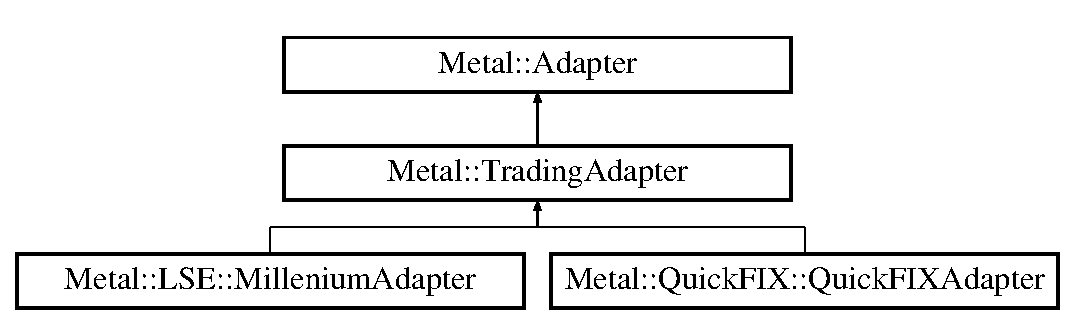
\includegraphics[height=3.000000cm]{classMetal_1_1Adapter}
\end{center}
\end{figure}
\subsection*{Public Member Functions}
\begin{DoxyCompactItemize}
\item 
\hyperlink{classMetal_1_1Adapter_a04519bef3780569a6e1bd26865b69577}{Adapter} (const std\+::string \&name\+Param, const std\+::string \&uuid\+Param)
\item 
\hypertarget{classMetal_1_1Adapter_a548dd70ecda0b21ddf3a459719d10377}{}const std\+::string \& {\bfseries get\+Name} ()\label{classMetal_1_1Adapter_a548dd70ecda0b21ddf3a459719d10377}

\item 
const std\+::string \& \hyperlink{classMetal_1_1Adapter_acd274a92f404cdc435a4d7030a7b1b58}{get\+U\+U\+I\+D} ()
\item 
\hypertarget{classMetal_1_1Adapter_a2c51b1d584d5110384782e4d535f52dc}{}virtual void {\bfseries start} ()=0\label{classMetal_1_1Adapter_a2c51b1d584d5110384782e4d535f52dc}

\item 
\hypertarget{classMetal_1_1Adapter_afac53c6c3aa80b5d09519b1daa0ccf86}{}virtual void {\bfseries stop} ()=0\label{classMetal_1_1Adapter_afac53c6c3aa80b5d09519b1daa0ccf86}

\end{DoxyCompactItemize}
\subsection*{Protected Attributes}
\begin{DoxyCompactItemize}
\item 
\hypertarget{classMetal_1_1Adapter_a6f0924d1c38de9c07c2fee73ce75d5f6}{}std\+::string {\bfseries name}\label{classMetal_1_1Adapter_a6f0924d1c38de9c07c2fee73ce75d5f6}

\item 
\hypertarget{classMetal_1_1Adapter_a20096a0f4ad14b746ca2e1f58ac4a969}{}std\+::string {\bfseries uuid}\label{classMetal_1_1Adapter_a20096a0f4ad14b746ca2e1f58ac4a969}

\end{DoxyCompactItemize}


\subsection{Constructor \& Destructor Documentation}
\hypertarget{classMetal_1_1Adapter_a04519bef3780569a6e1bd26865b69577}{}\index{Metal\+::\+Adapter@{Metal\+::\+Adapter}!Adapter@{Adapter}}
\index{Adapter@{Adapter}!Metal\+::\+Adapter@{Metal\+::\+Adapter}}
\subsubsection[{Adapter}]{\setlength{\rightskip}{0pt plus 5cm}Metal\+::\+Adapter\+::\+Adapter (
\begin{DoxyParamCaption}
\item[{const std\+::string \&}]{name\+Param, }
\item[{const std\+::string \&}]{uuid\+Param}
\end{DoxyParamCaption}
)\hspace{0.3cm}{\ttfamily [inline]}}\label{classMetal_1_1Adapter_a04519bef3780569a6e1bd26865b69577}

\begin{DoxyParams}{Parameters}
{\em } & \\
\hline
\end{DoxyParams}


\subsection{Member Function Documentation}
\hypertarget{classMetal_1_1Adapter_acd274a92f404cdc435a4d7030a7b1b58}{}\index{Metal\+::\+Adapter@{Metal\+::\+Adapter}!get\+U\+U\+I\+D@{get\+U\+U\+I\+D}}
\index{get\+U\+U\+I\+D@{get\+U\+U\+I\+D}!Metal\+::\+Adapter@{Metal\+::\+Adapter}}
\subsubsection[{get\+U\+U\+I\+D}]{\setlength{\rightskip}{0pt plus 5cm}const std\+::string\& Metal\+::\+Adapter\+::get\+U\+U\+I\+D (
\begin{DoxyParamCaption}
{}
\end{DoxyParamCaption}
)\hspace{0.3cm}{\ttfamily [inline]}}\label{classMetal_1_1Adapter_acd274a92f404cdc435a4d7030a7b1b58}
Retrieve Unique I\+D For example, this is used by benchmarking to report results~\newline
 This is also used on the web site to identify adapters. 

The documentation for this class was generated from the following file\+:\begin{DoxyCompactItemize}
\item 
/home/jc/metal/src/metal/Adapter.\+h\end{DoxyCompactItemize}

\hypertarget{classMetal_1_1Codec}{}\section{Metal\+:\+:Codec Class Reference}
\label{classMetal_1_1Codec}\index{Metal\+::\+Codec@{Metal\+::\+Codec}}


{\ttfamily \#include $<$Codec.\+h$>$}

Inheritance diagram for Metal\+:\+:Codec\+:\begin{figure}[H]
\begin{center}
\leavevmode
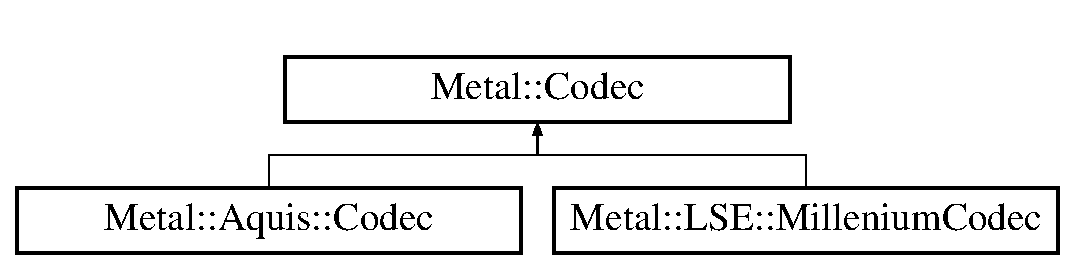
\includegraphics[height=2.000000cm]{classMetal_1_1Codec}
\end{center}
\end{figure}
\subsection*{Public Member Functions}
\begin{DoxyCompactItemize}
\item 
\hyperlink{classMetal_1_1Codec_a439fd8e827fabe656f49a7a043ab98d0}{Codec} ()
\item 
virtual int \hyperlink{classMetal_1_1Codec_a4d532631bde9029d9b5875fccaa5934e}{get\+Message\+Length} (char $\ast$data, int size)
\item 
void \hyperlink{classMetal_1_1Codec_a5b9970f32f2ff95981794993e2293011}{decode} (const char $\ast$data, int position, int8\+\_\+t \&output)
\item 
void \hyperlink{classMetal_1_1Codec_abf3b5c0af60d724c810b72b7dec909ee}{decode} (const char $\ast$data, int position, uint8\+\_\+t \&output)
\item 
void \hyperlink{classMetal_1_1Codec_a3f6d5f3018ae686f80512ad88e9a3329}{decode\+B\+E} (const char $\ast$data, int position, int16\+\_\+t \&output)
\item 
void \hyperlink{classMetal_1_1Codec_a2d51b5e2c7ab2d27ab12de4ac62e9eca}{decode\+B\+E} (const char $\ast$data, int position, uint16\+\_\+t \&output)
\item 
void \hyperlink{classMetal_1_1Codec_aa858a2edfd1227118d696f906746e7a1}{decode\+B\+E} (const char $\ast$data, int position, int32\+\_\+t \&output)
\item 
void \hyperlink{classMetal_1_1Codec_a84257d127b1918965b47e7df825fcfcb}{decode\+B\+E} (const char $\ast$data, int position, uint32\+\_\+t \&output)
\item 
void \hyperlink{classMetal_1_1Codec_a992488cf4e72ff2e26644ee0b719d7a3}{decode\+B\+E} (const char $\ast$data, int position, int64\+\_\+t \&output)
\item 
void \hyperlink{classMetal_1_1Codec_a4af4488934bd2dd20dcc82fbef75cca5}{decode\+B\+E} (const char $\ast$data, int position, uint64\+\_\+t \&output)
\item 
void \hyperlink{classMetal_1_1Codec_a9de32d0f9bbd0c25d3970b1fd748eb08}{decode\+L\+E} (const char $\ast$data, int position, int16\+\_\+t \&output)
\item 
void \hyperlink{classMetal_1_1Codec_afc62b66910d365f4cddcdc2d869371ea}{decode\+L\+E} (const char $\ast$data, int position, uint16\+\_\+t \&output)
\item 
void \hyperlink{classMetal_1_1Codec_ac8f4b899ca5f19400e7acbbf8ba28f33}{decode\+L\+E} (const char $\ast$data, int position, int32\+\_\+t \&output)
\item 
void \hyperlink{classMetal_1_1Codec_aa698a26f90f1f2874183c7b7c90c7b61}{decode\+L\+E} (const char $\ast$data, int position, uint32\+\_\+t \&output)
\item 
void \hyperlink{classMetal_1_1Codec_a1836678a806c987d7d96587a5130b3c6}{decode\+L\+E} (const char $\ast$data, int position, int64\+\_\+t \&output)
\item 
void \hyperlink{classMetal_1_1Codec_ae69549741e857cce3b915c9ef6ab6a7b}{decode\+L\+E} (const char $\ast$data, int position, uint64\+\_\+t \&output)
\item 
void \hyperlink{classMetal_1_1Codec_a22284aa82f334f7e81755dc044e05c58}{decode} (const char $\ast$data, int position, std\+::string \&output, int max\+Length)
\item 
void \hyperlink{classMetal_1_1Codec_aa6be9650e0fc53f01f1c94a771300665}{encode} (const std\+::string \&str, \hyperlink{classMetal_1_1Message}{Message} \&msg, int position, int max\+Length)
\item 
void \hyperlink{classMetal_1_1Codec_a2483a02d8022a4aae4345758244a154b}{encode} (const int8\+\_\+t \&i, \hyperlink{classMetal_1_1Message}{Message} \&msg, int position)
\item 
void \hyperlink{classMetal_1_1Codec_a638c8eccf2d989ea31a0670764b9cb0b}{encode\+L\+E} (const int16\+\_\+t \&i, \hyperlink{classMetal_1_1Message}{Message} \&msg, int position)
\item 
void \hyperlink{classMetal_1_1Codec_a08aafff1f98ec3d4b3c0490606d109f6}{encode\+L\+E} (const uint16\+\_\+t \&i, \hyperlink{classMetal_1_1Message}{Message} \&msg, int position)
\item 
void \hyperlink{classMetal_1_1Codec_a0c3cf0c6a614610c1d56859ea3fadc48}{encode\+B\+E} (const int16\+\_\+t \&i, \hyperlink{classMetal_1_1Message}{Message} \&msg, int position)
\item 
void \hyperlink{classMetal_1_1Codec_a188c8fdc0fb07affe85c8141a5314017}{encode\+B\+E} (const uint16\+\_\+t \&i, \hyperlink{classMetal_1_1Message}{Message} \&msg, int position)
\item 
void \hyperlink{classMetal_1_1Codec_a312401c93d9fdc7ec9468e87534c2f90}{encode\+L\+E} (const int32\+\_\+t \&i, \hyperlink{classMetal_1_1Message}{Message} \&msg, int position)
\item 
void \hyperlink{classMetal_1_1Codec_a5713bcd5042c5ded9e71a336f0ad42bf}{encode\+L\+E} (const uint32\+\_\+t \&i, \hyperlink{classMetal_1_1Message}{Message} \&msg, int position)
\item 
void \hyperlink{classMetal_1_1Codec_a30d84ca7c8a95a10103555b0364d3c0b}{encode\+B\+E} (const int32\+\_\+t \&i, \hyperlink{classMetal_1_1Message}{Message} \&msg, int position)
\item 
void \hyperlink{classMetal_1_1Codec_aa721fe0d642e0a6f127a2c1fc7410293}{encode\+B\+E} (const uint32\+\_\+t \&i, \hyperlink{classMetal_1_1Message}{Message} \&msg, int position)
\item 
void \hyperlink{classMetal_1_1Codec_a32a01360f4aff4c57a7c54c72e1e8a27}{encode\+L\+E} (const int64\+\_\+t \&i, \hyperlink{classMetal_1_1Message}{Message} \&msg, int position)
\item 
void \hyperlink{classMetal_1_1Codec_acbe0a9a61a63cbfc4373b1e72603a70f}{encode\+L\+E} (const uint64\+\_\+t \&i, \hyperlink{classMetal_1_1Message}{Message} \&msg, int position)
\item 
void \hyperlink{classMetal_1_1Codec_afd8c4138467dd3e593e17fe2cbd41a01}{encode\+B\+E} (const int64\+\_\+t \&i, \hyperlink{classMetal_1_1Message}{Message} \&msg, int position)
\item 
void \hyperlink{classMetal_1_1Codec_ae8e4c0fcd43cb06917f833f66e59b413}{encode\+B\+E} (const uint64\+\_\+t \&i, \hyperlink{classMetal_1_1Message}{Message} \&msg, int position)
\item 
virtual void \hyperlink{classMetal_1_1Codec_ae4796fc3d128fa650e28acdfe4277bd7}{encode\+Heart\+Beat} (\hyperlink{classMetal_1_1Message}{Message} \&msg)
\item 
virtual void \hyperlink{classMetal_1_1Codec_a14c3cc3c624726297171e843da71fa83}{encode\+Logon} (\hyperlink{classMetal_1_1Message}{Message} \&msg)
\item 
virtual \hyperlink{classMetal_1_1Codec_a68847484c9c80e04e4e4e5592cf113db}{$\sim$\+Codec} ()
\end{DoxyCompactItemize}
\subsection*{Static Public Member Functions}
\begin{DoxyCompactItemize}
\item 
static std\+::string \hyperlink{classMetal_1_1Codec_afe39c79b73724a05feea4c06a59b4d53}{format\+Hex} (char $\ast$data, int length)
\end{DoxyCompactItemize}


\subsection{Constructor \& Destructor Documentation}
\hypertarget{classMetal_1_1Codec_a439fd8e827fabe656f49a7a043ab98d0}{}\index{Metal\+::\+Codec@{Metal\+::\+Codec}!Codec@{Codec}}
\index{Codec@{Codec}!Metal\+::\+Codec@{Metal\+::\+Codec}}
\subsubsection[{Codec}]{\setlength{\rightskip}{0pt plus 5cm}Metal\+::\+Codec\+::\+Codec (
\begin{DoxyParamCaption}
{}
\end{DoxyParamCaption}
)}\label{classMetal_1_1Codec_a439fd8e827fabe656f49a7a043ab98d0}
\hypertarget{classMetal_1_1Codec_a68847484c9c80e04e4e4e5592cf113db}{}\index{Metal\+::\+Codec@{Metal\+::\+Codec}!````~Codec@{$\sim$\+Codec}}
\index{````~Codec@{$\sim$\+Codec}!Metal\+::\+Codec@{Metal\+::\+Codec}}
\subsubsection[{$\sim$\+Codec}]{\setlength{\rightskip}{0pt plus 5cm}Metal\+::\+Codec\+::$\sim$\+Codec (
\begin{DoxyParamCaption}
{}
\end{DoxyParamCaption}
)\hspace{0.3cm}{\ttfamily [virtual]}}\label{classMetal_1_1Codec_a68847484c9c80e04e4e4e5592cf113db}


Reimplemented in \hyperlink{classMetal_1_1Aquis_1_1Codec_a7bdeb61cbb583a2a77476cd7b196c0c2}{Metal\+::\+Aquis\+::\+Codec}.



\subsection{Member Function Documentation}
\hypertarget{classMetal_1_1Codec_a5b9970f32f2ff95981794993e2293011}{}\index{Metal\+::\+Codec@{Metal\+::\+Codec}!decode@{decode}}
\index{decode@{decode}!Metal\+::\+Codec@{Metal\+::\+Codec}}
\subsubsection[{decode}]{\setlength{\rightskip}{0pt plus 5cm}void Metal\+::\+Codec\+::decode (
\begin{DoxyParamCaption}
\item[{const char $\ast$}]{data, }
\item[{int}]{position, }
\item[{int8\+\_\+t \&}]{output}
\end{DoxyParamCaption}
)\hspace{0.3cm}{\ttfamily [inline]}}\label{classMetal_1_1Codec_a5b9970f32f2ff95981794993e2293011}
Decodes a 8 bits integer from a message \hypertarget{classMetal_1_1Codec_abf3b5c0af60d724c810b72b7dec909ee}{}\index{Metal\+::\+Codec@{Metal\+::\+Codec}!decode@{decode}}
\index{decode@{decode}!Metal\+::\+Codec@{Metal\+::\+Codec}}
\subsubsection[{decode}]{\setlength{\rightskip}{0pt plus 5cm}void Metal\+::\+Codec\+::decode (
\begin{DoxyParamCaption}
\item[{const char $\ast$}]{data, }
\item[{int}]{position, }
\item[{uint8\+\_\+t \&}]{output}
\end{DoxyParamCaption}
)\hspace{0.3cm}{\ttfamily [inline]}}\label{classMetal_1_1Codec_abf3b5c0af60d724c810b72b7dec909ee}
Decodes a 8 bits integer from a message \hypertarget{classMetal_1_1Codec_a22284aa82f334f7e81755dc044e05c58}{}\index{Metal\+::\+Codec@{Metal\+::\+Codec}!decode@{decode}}
\index{decode@{decode}!Metal\+::\+Codec@{Metal\+::\+Codec}}
\subsubsection[{decode}]{\setlength{\rightskip}{0pt plus 5cm}void Metal\+::\+Codec\+::decode (
\begin{DoxyParamCaption}
\item[{const char $\ast$}]{data, }
\item[{int}]{position, }
\item[{std\+::string \&}]{output, }
\item[{int}]{max\+Length}
\end{DoxyParamCaption}
)\hspace{0.3cm}{\ttfamily [inline]}}\label{classMetal_1_1Codec_a22284aa82f334f7e81755dc044e05c58}
Copies data into a string \hypertarget{classMetal_1_1Codec_a3f6d5f3018ae686f80512ad88e9a3329}{}\index{Metal\+::\+Codec@{Metal\+::\+Codec}!decode\+B\+E@{decode\+B\+E}}
\index{decode\+B\+E@{decode\+B\+E}!Metal\+::\+Codec@{Metal\+::\+Codec}}
\subsubsection[{decode\+B\+E}]{\setlength{\rightskip}{0pt plus 5cm}void Metal\+::\+Codec\+::decode\+B\+E (
\begin{DoxyParamCaption}
\item[{const char $\ast$}]{data, }
\item[{int}]{position, }
\item[{int16\+\_\+t \&}]{output}
\end{DoxyParamCaption}
)\hspace{0.3cm}{\ttfamily [inline]}}\label{classMetal_1_1Codec_a3f6d5f3018ae686f80512ad88e9a3329}
Decodes a 16 bits integer from a message in big endian format \hypertarget{classMetal_1_1Codec_a2d51b5e2c7ab2d27ab12de4ac62e9eca}{}\index{Metal\+::\+Codec@{Metal\+::\+Codec}!decode\+B\+E@{decode\+B\+E}}
\index{decode\+B\+E@{decode\+B\+E}!Metal\+::\+Codec@{Metal\+::\+Codec}}
\subsubsection[{decode\+B\+E}]{\setlength{\rightskip}{0pt plus 5cm}void Metal\+::\+Codec\+::decode\+B\+E (
\begin{DoxyParamCaption}
\item[{const char $\ast$}]{data, }
\item[{int}]{position, }
\item[{uint16\+\_\+t \&}]{output}
\end{DoxyParamCaption}
)\hspace{0.3cm}{\ttfamily [inline]}}\label{classMetal_1_1Codec_a2d51b5e2c7ab2d27ab12de4ac62e9eca}
Decodes an unsigned 16 bits integer from a message in big endian format \hypertarget{classMetal_1_1Codec_aa858a2edfd1227118d696f906746e7a1}{}\index{Metal\+::\+Codec@{Metal\+::\+Codec}!decode\+B\+E@{decode\+B\+E}}
\index{decode\+B\+E@{decode\+B\+E}!Metal\+::\+Codec@{Metal\+::\+Codec}}
\subsubsection[{decode\+B\+E}]{\setlength{\rightskip}{0pt plus 5cm}void Metal\+::\+Codec\+::decode\+B\+E (
\begin{DoxyParamCaption}
\item[{const char $\ast$}]{data, }
\item[{int}]{position, }
\item[{int32\+\_\+t \&}]{output}
\end{DoxyParamCaption}
)\hspace{0.3cm}{\ttfamily [inline]}}\label{classMetal_1_1Codec_aa858a2edfd1227118d696f906746e7a1}
Decodes a 32 bits integer from a message in big endian format \hypertarget{classMetal_1_1Codec_a84257d127b1918965b47e7df825fcfcb}{}\index{Metal\+::\+Codec@{Metal\+::\+Codec}!decode\+B\+E@{decode\+B\+E}}
\index{decode\+B\+E@{decode\+B\+E}!Metal\+::\+Codec@{Metal\+::\+Codec}}
\subsubsection[{decode\+B\+E}]{\setlength{\rightskip}{0pt plus 5cm}void Metal\+::\+Codec\+::decode\+B\+E (
\begin{DoxyParamCaption}
\item[{const char $\ast$}]{data, }
\item[{int}]{position, }
\item[{uint32\+\_\+t \&}]{output}
\end{DoxyParamCaption}
)\hspace{0.3cm}{\ttfamily [inline]}}\label{classMetal_1_1Codec_a84257d127b1918965b47e7df825fcfcb}
Decodes an unsigned 32 bits integer from a message in big endian format \hypertarget{classMetal_1_1Codec_a992488cf4e72ff2e26644ee0b719d7a3}{}\index{Metal\+::\+Codec@{Metal\+::\+Codec}!decode\+B\+E@{decode\+B\+E}}
\index{decode\+B\+E@{decode\+B\+E}!Metal\+::\+Codec@{Metal\+::\+Codec}}
\subsubsection[{decode\+B\+E}]{\setlength{\rightskip}{0pt plus 5cm}void Metal\+::\+Codec\+::decode\+B\+E (
\begin{DoxyParamCaption}
\item[{const char $\ast$}]{data, }
\item[{int}]{position, }
\item[{int64\+\_\+t \&}]{output}
\end{DoxyParamCaption}
)\hspace{0.3cm}{\ttfamily [inline]}}\label{classMetal_1_1Codec_a992488cf4e72ff2e26644ee0b719d7a3}
Decodes a 64 bits integer from a message in big endian format \hypertarget{classMetal_1_1Codec_a4af4488934bd2dd20dcc82fbef75cca5}{}\index{Metal\+::\+Codec@{Metal\+::\+Codec}!decode\+B\+E@{decode\+B\+E}}
\index{decode\+B\+E@{decode\+B\+E}!Metal\+::\+Codec@{Metal\+::\+Codec}}
\subsubsection[{decode\+B\+E}]{\setlength{\rightskip}{0pt plus 5cm}void Metal\+::\+Codec\+::decode\+B\+E (
\begin{DoxyParamCaption}
\item[{const char $\ast$}]{data, }
\item[{int}]{position, }
\item[{uint64\+\_\+t \&}]{output}
\end{DoxyParamCaption}
)\hspace{0.3cm}{\ttfamily [inline]}}\label{classMetal_1_1Codec_a4af4488934bd2dd20dcc82fbef75cca5}
Decodes a 64 bits integer from a message in big endian format \hypertarget{classMetal_1_1Codec_a9de32d0f9bbd0c25d3970b1fd748eb08}{}\index{Metal\+::\+Codec@{Metal\+::\+Codec}!decode\+L\+E@{decode\+L\+E}}
\index{decode\+L\+E@{decode\+L\+E}!Metal\+::\+Codec@{Metal\+::\+Codec}}
\subsubsection[{decode\+L\+E}]{\setlength{\rightskip}{0pt plus 5cm}void Metal\+::\+Codec\+::decode\+L\+E (
\begin{DoxyParamCaption}
\item[{const char $\ast$}]{data, }
\item[{int}]{position, }
\item[{int16\+\_\+t \&}]{output}
\end{DoxyParamCaption}
)\hspace{0.3cm}{\ttfamily [inline]}}\label{classMetal_1_1Codec_a9de32d0f9bbd0c25d3970b1fd748eb08}
Decodes a 16 bits integer from a message in little endian format \hypertarget{classMetal_1_1Codec_afc62b66910d365f4cddcdc2d869371ea}{}\index{Metal\+::\+Codec@{Metal\+::\+Codec}!decode\+L\+E@{decode\+L\+E}}
\index{decode\+L\+E@{decode\+L\+E}!Metal\+::\+Codec@{Metal\+::\+Codec}}
\subsubsection[{decode\+L\+E}]{\setlength{\rightskip}{0pt plus 5cm}void Metal\+::\+Codec\+::decode\+L\+E (
\begin{DoxyParamCaption}
\item[{const char $\ast$}]{data, }
\item[{int}]{position, }
\item[{uint16\+\_\+t \&}]{output}
\end{DoxyParamCaption}
)\hspace{0.3cm}{\ttfamily [inline]}}\label{classMetal_1_1Codec_afc62b66910d365f4cddcdc2d869371ea}
Decodes a 16 bits integer from a message in little endian format \hypertarget{classMetal_1_1Codec_ac8f4b899ca5f19400e7acbbf8ba28f33}{}\index{Metal\+::\+Codec@{Metal\+::\+Codec}!decode\+L\+E@{decode\+L\+E}}
\index{decode\+L\+E@{decode\+L\+E}!Metal\+::\+Codec@{Metal\+::\+Codec}}
\subsubsection[{decode\+L\+E}]{\setlength{\rightskip}{0pt plus 5cm}void Metal\+::\+Codec\+::decode\+L\+E (
\begin{DoxyParamCaption}
\item[{const char $\ast$}]{data, }
\item[{int}]{position, }
\item[{int32\+\_\+t \&}]{output}
\end{DoxyParamCaption}
)\hspace{0.3cm}{\ttfamily [inline]}}\label{classMetal_1_1Codec_ac8f4b899ca5f19400e7acbbf8ba28f33}
Decodes a 32 bits integer from a message in little endian format \hypertarget{classMetal_1_1Codec_aa698a26f90f1f2874183c7b7c90c7b61}{}\index{Metal\+::\+Codec@{Metal\+::\+Codec}!decode\+L\+E@{decode\+L\+E}}
\index{decode\+L\+E@{decode\+L\+E}!Metal\+::\+Codec@{Metal\+::\+Codec}}
\subsubsection[{decode\+L\+E}]{\setlength{\rightskip}{0pt plus 5cm}void Metal\+::\+Codec\+::decode\+L\+E (
\begin{DoxyParamCaption}
\item[{const char $\ast$}]{data, }
\item[{int}]{position, }
\item[{uint32\+\_\+t \&}]{output}
\end{DoxyParamCaption}
)\hspace{0.3cm}{\ttfamily [inline]}}\label{classMetal_1_1Codec_aa698a26f90f1f2874183c7b7c90c7b61}
Decodes an unsigned 32 bits integer from a message in little endian format \hypertarget{classMetal_1_1Codec_a1836678a806c987d7d96587a5130b3c6}{}\index{Metal\+::\+Codec@{Metal\+::\+Codec}!decode\+L\+E@{decode\+L\+E}}
\index{decode\+L\+E@{decode\+L\+E}!Metal\+::\+Codec@{Metal\+::\+Codec}}
\subsubsection[{decode\+L\+E}]{\setlength{\rightskip}{0pt plus 5cm}void Metal\+::\+Codec\+::decode\+L\+E (
\begin{DoxyParamCaption}
\item[{const char $\ast$}]{data, }
\item[{int}]{position, }
\item[{int64\+\_\+t \&}]{output}
\end{DoxyParamCaption}
)\hspace{0.3cm}{\ttfamily [inline]}}\label{classMetal_1_1Codec_a1836678a806c987d7d96587a5130b3c6}
Decodes a 64 bits integer from a message in little endian format \hypertarget{classMetal_1_1Codec_ae69549741e857cce3b915c9ef6ab6a7b}{}\index{Metal\+::\+Codec@{Metal\+::\+Codec}!decode\+L\+E@{decode\+L\+E}}
\index{decode\+L\+E@{decode\+L\+E}!Metal\+::\+Codec@{Metal\+::\+Codec}}
\subsubsection[{decode\+L\+E}]{\setlength{\rightskip}{0pt plus 5cm}void Metal\+::\+Codec\+::decode\+L\+E (
\begin{DoxyParamCaption}
\item[{const char $\ast$}]{data, }
\item[{int}]{position, }
\item[{uint64\+\_\+t \&}]{output}
\end{DoxyParamCaption}
)\hspace{0.3cm}{\ttfamily [inline]}}\label{classMetal_1_1Codec_ae69549741e857cce3b915c9ef6ab6a7b}
Decodes an unsigned 64 bits integer from a message in little endian format \hypertarget{classMetal_1_1Codec_aa6be9650e0fc53f01f1c94a771300665}{}\index{Metal\+::\+Codec@{Metal\+::\+Codec}!encode@{encode}}
\index{encode@{encode}!Metal\+::\+Codec@{Metal\+::\+Codec}}
\subsubsection[{encode}]{\setlength{\rightskip}{0pt plus 5cm}void Metal\+::\+Codec\+::encode (
\begin{DoxyParamCaption}
\item[{const std\+::string \&}]{str, }
\item[{{\bf Message} \&}]{msg, }
\item[{int}]{position, }
\item[{int}]{max\+Length}
\end{DoxyParamCaption}
)\hspace{0.3cm}{\ttfamily [inline]}}\label{classMetal_1_1Codec_aa6be9650e0fc53f01f1c94a771300665}
Encode a string up to the given length. 
\begin{DoxyParams}{Parameters}
{\em str} & String to be encoded \\
\hline
\end{DoxyParams}
\hypertarget{classMetal_1_1Codec_a2483a02d8022a4aae4345758244a154b}{}\index{Metal\+::\+Codec@{Metal\+::\+Codec}!encode@{encode}}
\index{encode@{encode}!Metal\+::\+Codec@{Metal\+::\+Codec}}
\subsubsection[{encode}]{\setlength{\rightskip}{0pt plus 5cm}void Metal\+::\+Codec\+::encode (
\begin{DoxyParamCaption}
\item[{const int8\+\_\+t \&}]{i, }
\item[{{\bf Message} \&}]{msg, }
\item[{int}]{position}
\end{DoxyParamCaption}
)\hspace{0.3cm}{\ttfamily [inline]}}\label{classMetal_1_1Codec_a2483a02d8022a4aae4345758244a154b}
\hypertarget{classMetal_1_1Codec_a0c3cf0c6a614610c1d56859ea3fadc48}{}\index{Metal\+::\+Codec@{Metal\+::\+Codec}!encode\+B\+E@{encode\+B\+E}}
\index{encode\+B\+E@{encode\+B\+E}!Metal\+::\+Codec@{Metal\+::\+Codec}}
\subsubsection[{encode\+B\+E}]{\setlength{\rightskip}{0pt plus 5cm}void Metal\+::\+Codec\+::encode\+B\+E (
\begin{DoxyParamCaption}
\item[{const int16\+\_\+t \&}]{i, }
\item[{{\bf Message} \&}]{msg, }
\item[{int}]{position}
\end{DoxyParamCaption}
)\hspace{0.3cm}{\ttfamily [inline]}}\label{classMetal_1_1Codec_a0c3cf0c6a614610c1d56859ea3fadc48}
\hypertarget{classMetal_1_1Codec_a188c8fdc0fb07affe85c8141a5314017}{}\index{Metal\+::\+Codec@{Metal\+::\+Codec}!encode\+B\+E@{encode\+B\+E}}
\index{encode\+B\+E@{encode\+B\+E}!Metal\+::\+Codec@{Metal\+::\+Codec}}
\subsubsection[{encode\+B\+E}]{\setlength{\rightskip}{0pt plus 5cm}void Metal\+::\+Codec\+::encode\+B\+E (
\begin{DoxyParamCaption}
\item[{const uint16\+\_\+t \&}]{i, }
\item[{{\bf Message} \&}]{msg, }
\item[{int}]{position}
\end{DoxyParamCaption}
)\hspace{0.3cm}{\ttfamily [inline]}}\label{classMetal_1_1Codec_a188c8fdc0fb07affe85c8141a5314017}
\hypertarget{classMetal_1_1Codec_a30d84ca7c8a95a10103555b0364d3c0b}{}\index{Metal\+::\+Codec@{Metal\+::\+Codec}!encode\+B\+E@{encode\+B\+E}}
\index{encode\+B\+E@{encode\+B\+E}!Metal\+::\+Codec@{Metal\+::\+Codec}}
\subsubsection[{encode\+B\+E}]{\setlength{\rightskip}{0pt plus 5cm}void Metal\+::\+Codec\+::encode\+B\+E (
\begin{DoxyParamCaption}
\item[{const int32\+\_\+t \&}]{i, }
\item[{{\bf Message} \&}]{msg, }
\item[{int}]{position}
\end{DoxyParamCaption}
)\hspace{0.3cm}{\ttfamily [inline]}}\label{classMetal_1_1Codec_a30d84ca7c8a95a10103555b0364d3c0b}
\hypertarget{classMetal_1_1Codec_aa721fe0d642e0a6f127a2c1fc7410293}{}\index{Metal\+::\+Codec@{Metal\+::\+Codec}!encode\+B\+E@{encode\+B\+E}}
\index{encode\+B\+E@{encode\+B\+E}!Metal\+::\+Codec@{Metal\+::\+Codec}}
\subsubsection[{encode\+B\+E}]{\setlength{\rightskip}{0pt plus 5cm}void Metal\+::\+Codec\+::encode\+B\+E (
\begin{DoxyParamCaption}
\item[{const uint32\+\_\+t \&}]{i, }
\item[{{\bf Message} \&}]{msg, }
\item[{int}]{position}
\end{DoxyParamCaption}
)\hspace{0.3cm}{\ttfamily [inline]}}\label{classMetal_1_1Codec_aa721fe0d642e0a6f127a2c1fc7410293}
\hypertarget{classMetal_1_1Codec_afd8c4138467dd3e593e17fe2cbd41a01}{}\index{Metal\+::\+Codec@{Metal\+::\+Codec}!encode\+B\+E@{encode\+B\+E}}
\index{encode\+B\+E@{encode\+B\+E}!Metal\+::\+Codec@{Metal\+::\+Codec}}
\subsubsection[{encode\+B\+E}]{\setlength{\rightskip}{0pt plus 5cm}void Metal\+::\+Codec\+::encode\+B\+E (
\begin{DoxyParamCaption}
\item[{const int64\+\_\+t \&}]{i, }
\item[{{\bf Message} \&}]{msg, }
\item[{int}]{position}
\end{DoxyParamCaption}
)\hspace{0.3cm}{\ttfamily [inline]}}\label{classMetal_1_1Codec_afd8c4138467dd3e593e17fe2cbd41a01}
\hypertarget{classMetal_1_1Codec_ae8e4c0fcd43cb06917f833f66e59b413}{}\index{Metal\+::\+Codec@{Metal\+::\+Codec}!encode\+B\+E@{encode\+B\+E}}
\index{encode\+B\+E@{encode\+B\+E}!Metal\+::\+Codec@{Metal\+::\+Codec}}
\subsubsection[{encode\+B\+E}]{\setlength{\rightskip}{0pt plus 5cm}void Metal\+::\+Codec\+::encode\+B\+E (
\begin{DoxyParamCaption}
\item[{const uint64\+\_\+t \&}]{i, }
\item[{{\bf Message} \&}]{msg, }
\item[{int}]{position}
\end{DoxyParamCaption}
)\hspace{0.3cm}{\ttfamily [inline]}}\label{classMetal_1_1Codec_ae8e4c0fcd43cb06917f833f66e59b413}
\hypertarget{classMetal_1_1Codec_ae4796fc3d128fa650e28acdfe4277bd7}{}\index{Metal\+::\+Codec@{Metal\+::\+Codec}!encode\+Heart\+Beat@{encode\+Heart\+Beat}}
\index{encode\+Heart\+Beat@{encode\+Heart\+Beat}!Metal\+::\+Codec@{Metal\+::\+Codec}}
\subsubsection[{encode\+Heart\+Beat}]{\setlength{\rightskip}{0pt plus 5cm}virtual void Metal\+::\+Codec\+::encode\+Heart\+Beat (
\begin{DoxyParamCaption}
\item[{{\bf Message} \&}]{msg}
\end{DoxyParamCaption}
)\hspace{0.3cm}{\ttfamily [inline]}, {\ttfamily [virtual]}}\label{classMetal_1_1Codec_ae4796fc3d128fa650e28acdfe4277bd7}
This method should be overriden for exchanges that require a heartbeat~\newline
 
\begin{DoxyParams}{Parameters}
{\em msg} & Where encoded Heart\+Beat \hyperlink{classMetal_1_1Message}{Message} will be stored \\
\hline
\end{DoxyParams}


Reimplemented in \hyperlink{classMetal_1_1LSE_1_1MilleniumCodec_a208c3b0765080cd8fe55b82f9df5a39f}{Metal\+::\+L\+S\+E\+::\+Millenium\+Codec}.

\hypertarget{classMetal_1_1Codec_a638c8eccf2d989ea31a0670764b9cb0b}{}\index{Metal\+::\+Codec@{Metal\+::\+Codec}!encode\+L\+E@{encode\+L\+E}}
\index{encode\+L\+E@{encode\+L\+E}!Metal\+::\+Codec@{Metal\+::\+Codec}}
\subsubsection[{encode\+L\+E}]{\setlength{\rightskip}{0pt plus 5cm}void Metal\+::\+Codec\+::encode\+L\+E (
\begin{DoxyParamCaption}
\item[{const int16\+\_\+t \&}]{i, }
\item[{{\bf Message} \&}]{msg, }
\item[{int}]{position}
\end{DoxyParamCaption}
)\hspace{0.3cm}{\ttfamily [inline]}}\label{classMetal_1_1Codec_a638c8eccf2d989ea31a0670764b9cb0b}
\hypertarget{classMetal_1_1Codec_a08aafff1f98ec3d4b3c0490606d109f6}{}\index{Metal\+::\+Codec@{Metal\+::\+Codec}!encode\+L\+E@{encode\+L\+E}}
\index{encode\+L\+E@{encode\+L\+E}!Metal\+::\+Codec@{Metal\+::\+Codec}}
\subsubsection[{encode\+L\+E}]{\setlength{\rightskip}{0pt plus 5cm}void Metal\+::\+Codec\+::encode\+L\+E (
\begin{DoxyParamCaption}
\item[{const uint16\+\_\+t \&}]{i, }
\item[{{\bf Message} \&}]{msg, }
\item[{int}]{position}
\end{DoxyParamCaption}
)\hspace{0.3cm}{\ttfamily [inline]}}\label{classMetal_1_1Codec_a08aafff1f98ec3d4b3c0490606d109f6}
\hypertarget{classMetal_1_1Codec_a312401c93d9fdc7ec9468e87534c2f90}{}\index{Metal\+::\+Codec@{Metal\+::\+Codec}!encode\+L\+E@{encode\+L\+E}}
\index{encode\+L\+E@{encode\+L\+E}!Metal\+::\+Codec@{Metal\+::\+Codec}}
\subsubsection[{encode\+L\+E}]{\setlength{\rightskip}{0pt plus 5cm}void Metal\+::\+Codec\+::encode\+L\+E (
\begin{DoxyParamCaption}
\item[{const int32\+\_\+t \&}]{i, }
\item[{{\bf Message} \&}]{msg, }
\item[{int}]{position}
\end{DoxyParamCaption}
)\hspace{0.3cm}{\ttfamily [inline]}}\label{classMetal_1_1Codec_a312401c93d9fdc7ec9468e87534c2f90}
\hypertarget{classMetal_1_1Codec_a5713bcd5042c5ded9e71a336f0ad42bf}{}\index{Metal\+::\+Codec@{Metal\+::\+Codec}!encode\+L\+E@{encode\+L\+E}}
\index{encode\+L\+E@{encode\+L\+E}!Metal\+::\+Codec@{Metal\+::\+Codec}}
\subsubsection[{encode\+L\+E}]{\setlength{\rightskip}{0pt plus 5cm}void Metal\+::\+Codec\+::encode\+L\+E (
\begin{DoxyParamCaption}
\item[{const uint32\+\_\+t \&}]{i, }
\item[{{\bf Message} \&}]{msg, }
\item[{int}]{position}
\end{DoxyParamCaption}
)\hspace{0.3cm}{\ttfamily [inline]}}\label{classMetal_1_1Codec_a5713bcd5042c5ded9e71a336f0ad42bf}
\hypertarget{classMetal_1_1Codec_a32a01360f4aff4c57a7c54c72e1e8a27}{}\index{Metal\+::\+Codec@{Metal\+::\+Codec}!encode\+L\+E@{encode\+L\+E}}
\index{encode\+L\+E@{encode\+L\+E}!Metal\+::\+Codec@{Metal\+::\+Codec}}
\subsubsection[{encode\+L\+E}]{\setlength{\rightskip}{0pt plus 5cm}void Metal\+::\+Codec\+::encode\+L\+E (
\begin{DoxyParamCaption}
\item[{const int64\+\_\+t \&}]{i, }
\item[{{\bf Message} \&}]{msg, }
\item[{int}]{position}
\end{DoxyParamCaption}
)\hspace{0.3cm}{\ttfamily [inline]}}\label{classMetal_1_1Codec_a32a01360f4aff4c57a7c54c72e1e8a27}
\hypertarget{classMetal_1_1Codec_acbe0a9a61a63cbfc4373b1e72603a70f}{}\index{Metal\+::\+Codec@{Metal\+::\+Codec}!encode\+L\+E@{encode\+L\+E}}
\index{encode\+L\+E@{encode\+L\+E}!Metal\+::\+Codec@{Metal\+::\+Codec}}
\subsubsection[{encode\+L\+E}]{\setlength{\rightskip}{0pt plus 5cm}void Metal\+::\+Codec\+::encode\+L\+E (
\begin{DoxyParamCaption}
\item[{const uint64\+\_\+t \&}]{i, }
\item[{{\bf Message} \&}]{msg, }
\item[{int}]{position}
\end{DoxyParamCaption}
)\hspace{0.3cm}{\ttfamily [inline]}}\label{classMetal_1_1Codec_acbe0a9a61a63cbfc4373b1e72603a70f}
\hypertarget{classMetal_1_1Codec_a14c3cc3c624726297171e843da71fa83}{}\index{Metal\+::\+Codec@{Metal\+::\+Codec}!encode\+Logon@{encode\+Logon}}
\index{encode\+Logon@{encode\+Logon}!Metal\+::\+Codec@{Metal\+::\+Codec}}
\subsubsection[{encode\+Logon}]{\setlength{\rightskip}{0pt plus 5cm}virtual void Metal\+::\+Codec\+::encode\+Logon (
\begin{DoxyParamCaption}
\item[{{\bf Message} \&}]{msg}
\end{DoxyParamCaption}
)\hspace{0.3cm}{\ttfamily [inline]}, {\ttfamily [virtual]}}\label{classMetal_1_1Codec_a14c3cc3c624726297171e843da71fa83}
This method should be overriden by exchanges that require a logon~\newline
 
\begin{DoxyParams}{Parameters}
{\em msg} & Where encoded \hyperlink{classMetal_1_1Logon}{Logon} \hyperlink{classMetal_1_1Message}{Message} will be stored \\
\hline
\end{DoxyParams}
\hypertarget{classMetal_1_1Codec_afe39c79b73724a05feea4c06a59b4d53}{}\index{Metal\+::\+Codec@{Metal\+::\+Codec}!format\+Hex@{format\+Hex}}
\index{format\+Hex@{format\+Hex}!Metal\+::\+Codec@{Metal\+::\+Codec}}
\subsubsection[{format\+Hex}]{\setlength{\rightskip}{0pt plus 5cm}std\+::string Metal\+::\+Codec\+::format\+Hex (
\begin{DoxyParamCaption}
\item[{char $\ast$}]{data, }
\item[{int}]{length}
\end{DoxyParamCaption}
)\hspace{0.3cm}{\ttfamily [static]}}\label{classMetal_1_1Codec_afe39c79b73724a05feea4c06a59b4d53}
\hypertarget{classMetal_1_1Codec_a4d532631bde9029d9b5875fccaa5934e}{}\index{Metal\+::\+Codec@{Metal\+::\+Codec}!get\+Message\+Length@{get\+Message\+Length}}
\index{get\+Message\+Length@{get\+Message\+Length}!Metal\+::\+Codec@{Metal\+::\+Codec}}
\subsubsection[{get\+Message\+Length}]{\setlength{\rightskip}{0pt plus 5cm}virtual int Metal\+::\+Codec\+::get\+Message\+Length (
\begin{DoxyParamCaption}
\item[{char $\ast$}]{data, }
\item[{int}]{size}
\end{DoxyParamCaption}
)\hspace{0.3cm}{\ttfamily [inline]}, {\ttfamily [virtual]}}\label{classMetal_1_1Codec_a4d532631bde9029d9b5875fccaa5934e}
Find out message length from its wire representation. Will find out message length and copy data into msg bytes. 
\begin{DoxyParams}{Parameters}
{\em data} & Byte array containing data \\
\hline
{\em size} & Number of bytes in array \\
\hline
\end{DoxyParams}
\begin{DoxyReturn}{Returns}
\hyperlink{classMetal_1_1Message}{Message} length or 0 if no message was found in data 
\end{DoxyReturn}


The documentation for this class was generated from the following files\+:\begin{DoxyCompactItemize}
\item 
/home/jc/metal/github/include/metal/\hyperlink{include_2metal_2Codec_8h}{Codec.\+h}\item 
/home/jc/metal/github/src/metal/\hyperlink{metal_2Codec_8cpp}{Codec.\+cpp}\end{DoxyCompactItemize}

\hypertarget{classDisplay}{}\section{Display Class Reference}
\label{classDisplay}\index{Display@{Display}}
\subsection*{Static Public Member Functions}
\begin{DoxyCompactItemize}
\item 
\hypertarget{classDisplay_add7183a29b473e35d3dc9b85172560e8}{}static void {\bfseries get\+C\+P\+U\+Description} (std\+::string \&str)\label{classDisplay_add7183a29b473e35d3dc9b85172560e8}

\item 
\hypertarget{classDisplay_a3bed00f180043a15209c9010e98aa874}{}static void {\bfseries get\+O\+S\+Description} (std\+::string \&str)\label{classDisplay_a3bed00f180043a15209c9010e98aa874}

\end{DoxyCompactItemize}


The documentation for this class was generated from the following files\+:\begin{DoxyCompactItemize}
\item 
/home/jc/metal/src/benchmark/Display.\+h\item 
/home/jc/metal/src/benchmark/Display.\+cpp\end{DoxyCompactItemize}

\hypertarget{classException}{}\section{Exception Class Reference}
\label{classException}\index{Exception@{Exception}}


{\ttfamily \#include $<$netlink/exception.\+h$>$}

\subsection*{Public Types}
\begin{DoxyCompactItemize}
\item 
\hypertarget{classException_a99403a9d2a44da7f414a2f3d4f23eca2}{}enum {\bfseries C\+O\+D\+E} \label{classException_a99403a9d2a44da7f414a2f3d4f23eca2}

\end{DoxyCompactItemize}
\subsection*{Public Member Functions}
\begin{DoxyCompactItemize}
\item 
\hypertarget{classException_aafcd1188d8e22205609c25b05d325ae0}{}{\bfseries Exception} (C\+O\+D\+E \hyperlink{classException_a3404e105d108beb97d9fb4b22d9fa04c}{code}, const string \&\hyperlink{classException_ad0b441605d8f410501d91d8e08ed7cfc}{msg}, int \hyperlink{classException_ac63a198ea817835198c53825c5809b3f}{native\+Error\+Code}=0)\label{classException_aafcd1188d8e22205609c25b05d325ae0}

\item 
C\+O\+D\+E \hyperlink{classException_a3404e105d108beb97d9fb4b22d9fa04c}{code} () const 
\item 
const string \& \hyperlink{classException_ad0b441605d8f410501d91d8e08ed7cfc}{msg} () const 
\item 
const char $\ast$ \hyperlink{classException_a45642915395d3b813fedc2593fbcb8bb}{what} () const 
\item 
int \hyperlink{classException_ac63a198ea817835198c53825c5809b3f}{native\+Error\+Code} () const 
\end{DoxyCompactItemize}


\subsection{Detailed Description}
\hyperlink{classException}{Exception} Class 

\subsection{Member Function Documentation}
\hypertarget{classException_a3404e105d108beb97d9fb4b22d9fa04c}{}\index{Exception@{Exception}!code@{code}}
\index{code@{code}!Exception@{Exception}}
\subsubsection[{code}]{\setlength{\rightskip}{0pt plus 5cm}C\+O\+D\+E Exception\+::code (
\begin{DoxyParamCaption}
{}
\end{DoxyParamCaption}
) const\hspace{0.3cm}{\ttfamily [inline]}}\label{classException_a3404e105d108beb97d9fb4b22d9fa04c}
Returns the error code\+:  \begin{DoxyReturn}{Returns}
Error code
\end{DoxyReturn}
\begin{DoxyNote}{Note}
Defined Error Codes\+: \begin{DoxyItemize}
\item B\+A\+D\+\_\+\+P\+R\+O\+T\+O\+C\+O\+L \item B\+A\+D\+\_\+\+I\+P\+\_\+\+V\+E\+R \item E\+R\+R\+O\+R\+\_\+\+I\+N\+I\+T \item E\+R\+R\+O\+R\+\_\+\+S\+E\+T\+\_\+\+A\+D\+D\+R\+\_\+\+I\+N\+F\+O \item E\+R\+R\+O\+R\+\_\+\+G\+E\+T\+\_\+\+A\+D\+D\+R\+\_\+\+I\+N\+F\+O \item E\+R\+R\+O\+R\+\_\+\+S\+E\+T\+\_\+\+S\+O\+C\+K\+\_\+\+O\+P\+T \item E\+R\+R\+O\+R\+\_\+\+C\+A\+N\+\_\+\+N\+O\+T\+\_\+\+L\+I\+S\+T\+E\+N \item E\+R\+R\+O\+R\+\_\+\+C\+O\+N\+N\+E\+C\+T\+\_\+\+S\+O\+C\+K\+E\+T \item E\+R\+R\+O\+R\+\_\+\+S\+E\+N\+D \item E\+R\+R\+O\+R\+\_\+\+R\+E\+A\+D \item E\+R\+R\+O\+R\+\_\+\+I\+O\+C\+T\+L \item E\+R\+R\+O\+R\+\_\+\+S\+E\+L\+E\+C\+T \item E\+R\+R\+O\+R\+\_\+\+A\+L\+L\+O\+C \item E\+X\+P\+E\+C\+T\+E\+D\+\_\+\+T\+C\+P\+\_\+\+S\+O\+C\+K\+E\+T \item E\+X\+P\+E\+C\+T\+E\+D\+\_\+\+U\+D\+P\+\_\+\+S\+O\+C\+K\+E\+T \item E\+X\+P\+E\+C\+T\+E\+D\+\_\+\+C\+L\+I\+E\+N\+T\+\_\+\+S\+O\+C\+K\+E\+T \item E\+X\+P\+E\+C\+T\+E\+D\+\_\+\+S\+E\+R\+V\+E\+R\+\_\+\+S\+O\+C\+K\+E\+T \item E\+X\+P\+E\+C\+T\+E\+D\+\_\+\+H\+O\+S\+T\+\_\+\+T\+O \item O\+U\+T\+\_\+\+O\+F\+\_\+\+R\+A\+N\+G\+E \end{DoxyItemize}

\end{DoxyNote}
\hypertarget{classException_ad0b441605d8f410501d91d8e08ed7cfc}{}\index{Exception@{Exception}!msg@{msg}}
\index{msg@{msg}!Exception@{Exception}}
\subsubsection[{msg}]{\setlength{\rightskip}{0pt plus 5cm}const string\& Exception\+::msg (
\begin{DoxyParamCaption}
{}
\end{DoxyParamCaption}
) const\hspace{0.3cm}{\ttfamily [inline]}}\label{classException_ad0b441605d8f410501d91d8e08ed7cfc}
Returns the error text message

\begin{DoxyReturn}{Returns}
A string with a human readable error description 
\end{DoxyReturn}
\hypertarget{classException_ac63a198ea817835198c53825c5809b3f}{}\index{Exception@{Exception}!native\+Error\+Code@{native\+Error\+Code}}
\index{native\+Error\+Code@{native\+Error\+Code}!Exception@{Exception}}
\subsubsection[{native\+Error\+Code}]{\setlength{\rightskip}{0pt plus 5cm}int Exception\+::native\+Error\+Code (
\begin{DoxyParamCaption}
{}
\end{DoxyParamCaption}
) const\hspace{0.3cm}{\ttfamily [inline]}}\label{classException_ac63a198ea817835198c53825c5809b3f}
Returns the native error code received.

\begin{DoxyReturn}{Returns}
Native error code set by O\+S 
\end{DoxyReturn}
\begin{DoxyWarning}{Warning}
Native error codes differ depending of the O\+S 
\end{DoxyWarning}
\hypertarget{classException_a45642915395d3b813fedc2593fbcb8bb}{}\index{Exception@{Exception}!what@{what}}
\index{what@{what}!Exception@{Exception}}
\subsubsection[{what}]{\setlength{\rightskip}{0pt plus 5cm}const char$\ast$ Exception\+::what (
\begin{DoxyParamCaption}
{}
\end{DoxyParamCaption}
) const\hspace{0.3cm}{\ttfamily [inline]}}\label{classException_a45642915395d3b813fedc2593fbcb8bb}
Returns the error text message

\begin{DoxyReturn}{Returns}
A C-\/string with a human readable error description 
\end{DoxyReturn}


The documentation for this class was generated from the following file\+:\begin{DoxyCompactItemize}
\item 
/home/jc/metal/src/net\+Link/include/netlink/exception.\+h\end{DoxyCompactItemize}

\hypertarget{classMetal_1_1Logon}{}\section{Metal\+:\+:Logon Class Reference}
\label{classMetal_1_1Logon}\index{Metal\+::\+Logon@{Metal\+::\+Logon}}


{\ttfamily \#include $<$metal.\+h$>$}



\subsection{Detailed Description}
This is the base for all logon messages 

The documentation for this class was generated from the following file\+:\begin{DoxyCompactItemize}
\item 
/home/jc/metal/github/include/metal/\hyperlink{metal_8h}{metal.\+h}\end{DoxyCompactItemize}

\hypertarget{classMetal_1_1LSE_1_1Logon}{}\section{Metal\+:\+:L\+S\+E\+:\+:Logon Class Reference}
\label{classMetal_1_1LSE_1_1Logon}\index{Metal\+::\+L\+S\+E\+::\+Logon@{Metal\+::\+L\+S\+E\+::\+Logon}}
\subsection*{Public Member Functions}
\begin{DoxyCompactItemize}
\item 
\hypertarget{classMetal_1_1LSE_1_1Logon_afdff6d189d154169b3f0c32a0ca1d134}{}{\bfseries Logon} (std\+::string user\+Name\+Param, std\+::string password\+Param, std\+::string new\+Password\+Param)\label{classMetal_1_1LSE_1_1Logon_afdff6d189d154169b3f0c32a0ca1d134}

\end{DoxyCompactItemize}
\subsection*{Public Attributes}
\begin{DoxyCompactItemize}
\item 
\hypertarget{classMetal_1_1LSE_1_1Logon_a10fa4ed887ed159b7157e5aab908b18f}{}std\+::string {\bfseries user\+Name}\label{classMetal_1_1LSE_1_1Logon_a10fa4ed887ed159b7157e5aab908b18f}

\item 
\hypertarget{classMetal_1_1LSE_1_1Logon_ae8181000986aeb93bf3e3b989fc238ae}{}std\+::string {\bfseries password}\label{classMetal_1_1LSE_1_1Logon_ae8181000986aeb93bf3e3b989fc238ae}

\item 
\hypertarget{classMetal_1_1LSE_1_1Logon_a53afe9b298d908d8580462e9af4cdd5a}{}std\+::string {\bfseries new\+Password}\label{classMetal_1_1LSE_1_1Logon_a53afe9b298d908d8580462e9af4cdd5a}

\end{DoxyCompactItemize}


The documentation for this class was generated from the following files\+:\begin{DoxyCompactItemize}
\item 
/home/jc/metal/src/metal/adapters/\+L\+S\+E\+Trading\+Adapter/Logon.\+h\item 
/home/jc/metal/src/metal/adapters/\+L\+S\+E\+Trading\+Adapter/Logon.\+cpp\end{DoxyCompactItemize}

\hypertarget{classMetal_1_1Mapper}{}\section{Metal\+:\+:Mapper Class Reference}
\label{classMetal_1_1Mapper}\index{Metal\+::\+Mapper@{Metal\+::\+Mapper}}
Inheritance diagram for Metal\+:\+:Mapper\+:\begin{figure}[H]
\begin{center}
\leavevmode
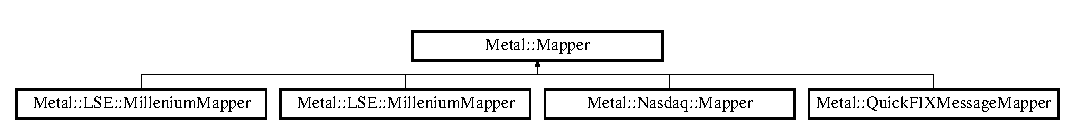
\includegraphics[height=2.000000cm]{classMetal_1_1Mapper}
\end{center}
\end{figure}


The documentation for this class was generated from the following files\+:\begin{DoxyCompactItemize}
\item 
/home/jc/metal/src/metal/Mapper.\+h\item 
/home/jc/metal/src/metal/Mapper.\+cpp\end{DoxyCompactItemize}

\hypertarget{classMetal_1_1MappingException}{}\section{Metal\+:\+:Mapping\+Exception Class Reference}
\label{classMetal_1_1MappingException}\index{Metal\+::\+Mapping\+Exception@{Metal\+::\+Mapping\+Exception}}
Inheritance diagram for Metal\+:\+:Mapping\+Exception\+:\begin{figure}[H]
\begin{center}
\leavevmode
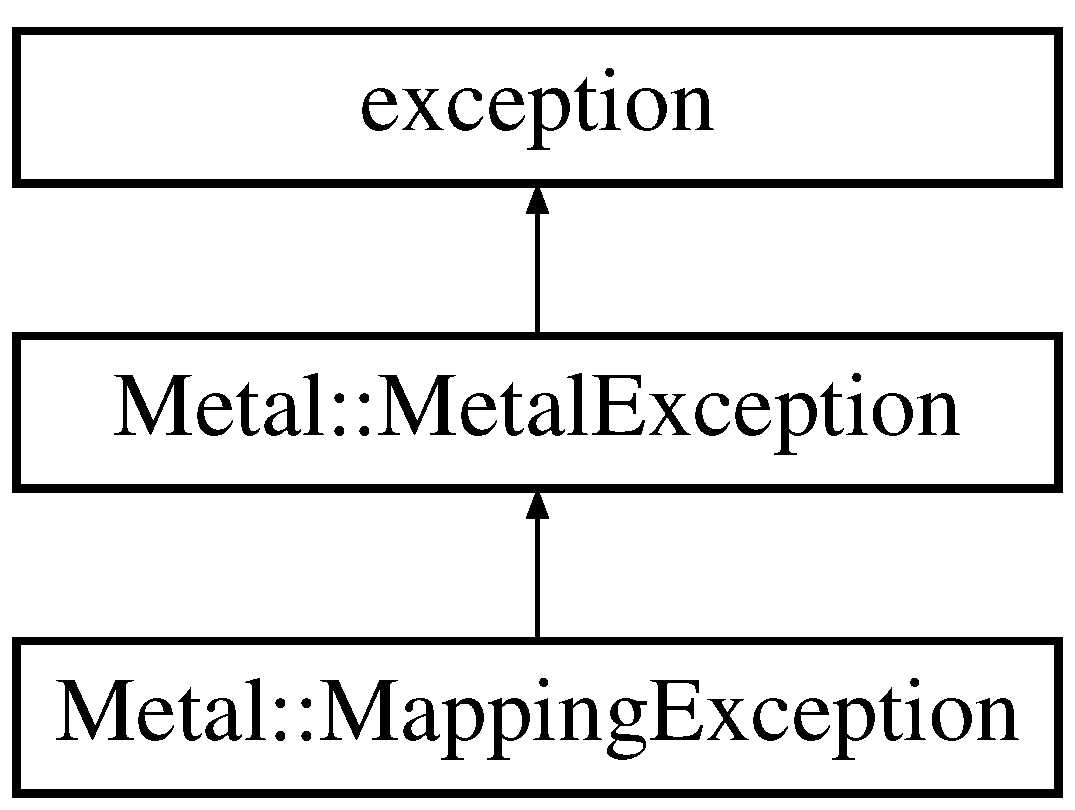
\includegraphics[height=3.000000cm]{classMetal_1_1MappingException}
\end{center}
\end{figure}
\subsection*{Public Member Functions}
\begin{DoxyCompactItemize}
\item 
\hypertarget{classMetal_1_1MappingException_ac343b35119e5515197df087da5fceeaf}{}{\bfseries Mapping\+Exception} (const std\+::string \&message)\label{classMetal_1_1MappingException_ac343b35119e5515197df087da5fceeaf}

\end{DoxyCompactItemize}


The documentation for this class was generated from the following file\+:\begin{DoxyCompactItemize}
\item 
/home/jc/metal/src/metal/Metal\+Exceptions.\+h\end{DoxyCompactItemize}

\hypertarget{classMetal_1_1Message}{}\section{Metal\+:\+:Message Class Reference}
\label{classMetal_1_1Message}\index{Metal\+::\+Message@{Metal\+::\+Message}}
\subsection*{Public Member Functions}
\begin{DoxyCompactItemize}
\item 
\hypertarget{classMetal_1_1Message_abc94615951dbde67368f977b717176fe}{}const char $\ast$ {\bfseries get\+Data} ()\label{classMetal_1_1Message_abc94615951dbde67368f977b717176fe}

\item 
\hypertarget{classMetal_1_1Message_a22984c81035306cfde91a575ac19d32a}{}const size\+\_\+t {\bfseries get\+Length} ()\label{classMetal_1_1Message_a22984c81035306cfde91a575ac19d32a}

\item 
void \hyperlink{classMetal_1_1Message_a9f9b7fb98dbe697d9cf7ad394fd45a2e}{set} (int position, char value)
\item 
void \hyperlink{classMetal_1_1Message_a7cb33179723ecc8a05860a97d9a518e3}{set} (int position, std\+::string str, int max\+Length)
\end{DoxyCompactItemize}


\subsection{Member Function Documentation}
\hypertarget{classMetal_1_1Message_a9f9b7fb98dbe697d9cf7ad394fd45a2e}{}\index{Metal\+::\+Message@{Metal\+::\+Message}!set@{set}}
\index{set@{set}!Metal\+::\+Message@{Metal\+::\+Message}}
\subsubsection[{set}]{\setlength{\rightskip}{0pt plus 5cm}void Metal\+::\+Message\+::set (
\begin{DoxyParamCaption}
\item[{int}]{position, }
\item[{char}]{value}
\end{DoxyParamCaption}
)\hspace{0.3cm}{\ttfamily [inline]}}\label{classMetal_1_1Message_a9f9b7fb98dbe697d9cf7ad394fd45a2e}
Write a single character at given position 
\begin{DoxyParams}{Parameters}
{\em position} & Where the character should be writted \\
\hline
{\em value} & Value to be written \\
\hline
\end{DoxyParams}
\hypertarget{classMetal_1_1Message_a7cb33179723ecc8a05860a97d9a518e3}{}\index{Metal\+::\+Message@{Metal\+::\+Message}!set@{set}}
\index{set@{set}!Metal\+::\+Message@{Metal\+::\+Message}}
\subsubsection[{set}]{\setlength{\rightskip}{0pt plus 5cm}void Metal\+::\+Message\+::set (
\begin{DoxyParamCaption}
\item[{int}]{position, }
\item[{std\+::string}]{str, }
\item[{int}]{max\+Length}
\end{DoxyParamCaption}
)\hspace{0.3cm}{\ttfamily [inline]}}\label{classMetal_1_1Message_a7cb33179723ecc8a05860a97d9a518e3}
Write a complete string at given position 
\begin{DoxyParams}{Parameters}
{\em position} & Where the string should be writted \\
\hline
{\em str} & String to be written \\
\hline
{\em max\+Length} & maximum length to be copied from the string \\
\hline
\end{DoxyParams}


The documentation for this class was generated from the following files\+:\begin{DoxyCompactItemize}
\item 
/home/jc/metal/src/metal/Message.\+h\item 
/home/jc/metal/src/metal/Message.\+cpp\end{DoxyCompactItemize}

\hypertarget{classMetal_1_1MetalException}{}\section{Metal\+:\+:Metal\+Exception Class Reference}
\label{classMetal_1_1MetalException}\index{Metal\+::\+Metal\+Exception@{Metal\+::\+Metal\+Exception}}
Inheritance diagram for Metal\+:\+:Metal\+Exception\+:\begin{figure}[H]
\begin{center}
\leavevmode
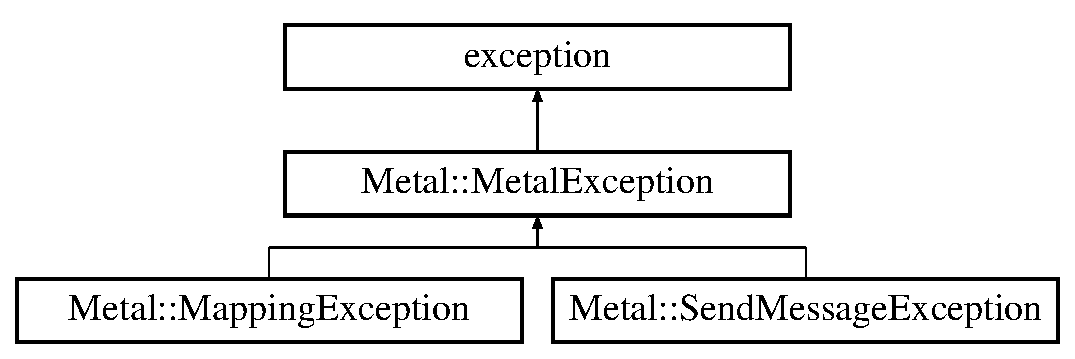
\includegraphics[height=3.000000cm]{classMetal_1_1MetalException}
\end{center}
\end{figure}
\subsection*{Public Member Functions}
\begin{DoxyCompactItemize}
\item 
\hypertarget{classMetal_1_1MetalException_afa58e4cd82c3aca7a138024fd1b6f090}{}{\bfseries Metal\+Exception} (const std\+::string \&message)\label{classMetal_1_1MetalException_afa58e4cd82c3aca7a138024fd1b6f090}

\item 
\hypertarget{classMetal_1_1MetalException_a74fa237bd4484764faccfbebd54801b5}{}virtual const char $\ast$ {\bfseries what} () const   throw ()\label{classMetal_1_1MetalException_a74fa237bd4484764faccfbebd54801b5}

\end{DoxyCompactItemize}


The documentation for this class was generated from the following file\+:\begin{DoxyCompactItemize}
\item 
/home/jc/metal/src/metal/Metal\+Exceptions.\+h\end{DoxyCompactItemize}

\hypertarget{classMetal_1_1LSE_1_1MilleniumAdapter}{}\section{Metal\+:\+:L\+S\+E\+:\+:Millenium\+Adapter Class Reference}
\label{classMetal_1_1LSE_1_1MilleniumAdapter}\index{Metal\+::\+L\+S\+E\+::\+Millenium\+Adapter@{Metal\+::\+L\+S\+E\+::\+Millenium\+Adapter}}
Inheritance diagram for Metal\+:\+:L\+S\+E\+:\+:Millenium\+Adapter\+:\begin{figure}[H]
\begin{center}
\leavevmode
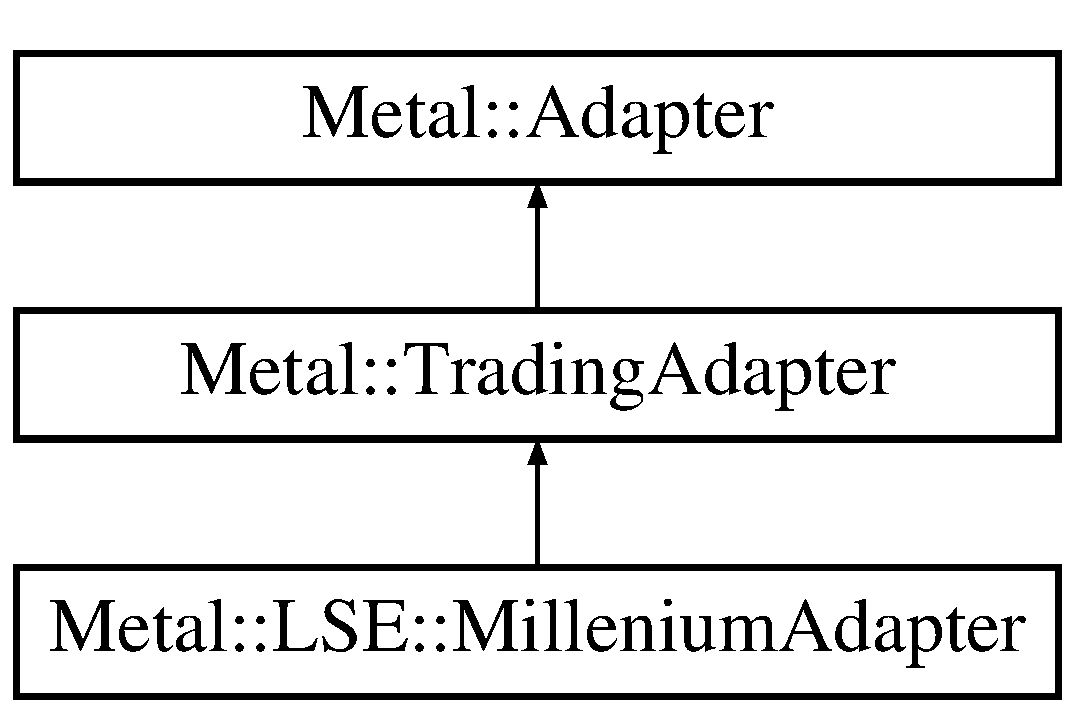
\includegraphics[height=3.000000cm]{classMetal_1_1LSE_1_1MilleniumAdapter}
\end{center}
\end{figure}
\subsection*{Public Member Functions}
\begin{DoxyCompactItemize}
\item 
void \hyperlink{classMetal_1_1LSE_1_1MilleniumAdapter_ab3da43142636043e0ade20b0881c9976}{send} (const \hyperlink{classMetal_1_1NewOrderSingle}{New\+Order\+Single} \&nos)
\item 
virtual void \hyperlink{classMetal_1_1LSE_1_1MilleniumAdapter_add4508b367a6383b42fb2fd1744946cd}{recv} (const Execution\+Report \&er)
\item 
\hypertarget{classMetal_1_1LSE_1_1MilleniumAdapter_a402c564b7a955fac6660e6bfeee66093}{}void {\bfseries start} ()\label{classMetal_1_1LSE_1_1MilleniumAdapter_a402c564b7a955fac6660e6bfeee66093}

\item 
\hypertarget{classMetal_1_1LSE_1_1MilleniumAdapter_acb5018d36915f34612958d87ad8325af}{}void {\bfseries stop} ()\label{classMetal_1_1LSE_1_1MilleniumAdapter_acb5018d36915f34612958d87ad8325af}

\item 
void \hyperlink{classMetal_1_1LSE_1_1MilleniumAdapter_ab4bba2e8403ae7ed5b335985b4295b9f}{send\+Logon} ()
\item 
void \hyperlink{classMetal_1_1LSE_1_1MilleniumAdapter_a01a0796b972925d6a430e2f788eec5ee}{benchmark} (const std\+::vector$<$ \hyperlink{classMetal_1_1NewOrderSingle}{Metal\+::\+New\+Order\+Single} $>$ \&, std\+::chrono\+::milliseconds \&mapping\+Duration, std\+::chrono\+::milliseconds \&encoding\+Duration)
\item 
void \hyperlink{classMetal_1_1LSE_1_1MilleniumAdapter_acdfc9b84439e745de42c0f72a1e22a67}{benchmark} (const std\+::vector$<$ \hyperlink{classMetal_1_1OrderCancelRequest}{Metal\+::\+Order\+Cancel\+Request} $>$ \&, std\+::chrono\+::milliseconds \&, std\+::chrono\+::milliseconds \&)
\end{DoxyCompactItemize}
\subsection*{Protected Attributes}
\begin{DoxyCompactItemize}
\item 
\hypertarget{classMetal_1_1LSE_1_1MilleniumAdapter_a1c12122da30ec79f3907a82ac1847c33}{}std\+::string {\bfseries user\+Name}\label{classMetal_1_1LSE_1_1MilleniumAdapter_a1c12122da30ec79f3907a82ac1847c33}

\item 
\hypertarget{classMetal_1_1LSE_1_1MilleniumAdapter_aa8120f11aac5d4825a5766d86e53e5a2}{}std\+::string {\bfseries password}\label{classMetal_1_1LSE_1_1MilleniumAdapter_aa8120f11aac5d4825a5766d86e53e5a2}

\end{DoxyCompactItemize}
\subsection*{Additional Inherited Members}


\subsection{Member Function Documentation}
\hypertarget{classMetal_1_1LSE_1_1MilleniumAdapter_a01a0796b972925d6a430e2f788eec5ee}{}\index{Metal\+::\+L\+S\+E\+::\+Millenium\+Adapter@{Metal\+::\+L\+S\+E\+::\+Millenium\+Adapter}!benchmark@{benchmark}}
\index{benchmark@{benchmark}!Metal\+::\+L\+S\+E\+::\+Millenium\+Adapter@{Metal\+::\+L\+S\+E\+::\+Millenium\+Adapter}}
\subsubsection[{benchmark}]{\setlength{\rightskip}{0pt plus 5cm}void Metal\+::\+L\+S\+E\+::\+Millenium\+Adapter\+::benchmark (
\begin{DoxyParamCaption}
\item[{const std\+::vector$<$ {\bf Metal\+::\+New\+Order\+Single} $>$ \&}]{, }
\item[{std\+::chrono\+::milliseconds \&}]{mapping\+Duration, }
\item[{std\+::chrono\+::milliseconds \&}]{encoding\+Duration}
\end{DoxyParamCaption}
)}\label{classMetal_1_1LSE_1_1MilleniumAdapter_a01a0796b972925d6a430e2f788eec5ee}
\begin{DoxySeeAlso}{See also}
\hyperlink{classMetal_1_1TradingAdapter_a161ad3db17091807d091d1b236de0105}{Trading\+Adapter\+::benchmark} 
\end{DoxySeeAlso}
\hypertarget{classMetal_1_1LSE_1_1MilleniumAdapter_acdfc9b84439e745de42c0f72a1e22a67}{}\index{Metal\+::\+L\+S\+E\+::\+Millenium\+Adapter@{Metal\+::\+L\+S\+E\+::\+Millenium\+Adapter}!benchmark@{benchmark}}
\index{benchmark@{benchmark}!Metal\+::\+L\+S\+E\+::\+Millenium\+Adapter@{Metal\+::\+L\+S\+E\+::\+Millenium\+Adapter}}
\subsubsection[{benchmark}]{\setlength{\rightskip}{0pt plus 5cm}void Metal\+::\+L\+S\+E\+::\+Millenium\+Adapter\+::benchmark (
\begin{DoxyParamCaption}
\item[{const std\+::vector$<$ {\bf Metal\+::\+Order\+Cancel\+Request} $>$ \&}]{all\+Cancels, }
\item[{std\+::chrono\+::milliseconds \&}]{mapping\+Duration, }
\item[{std\+::chrono\+::milliseconds \&}]{encoding\+Duration}
\end{DoxyParamCaption}
)}\label{classMetal_1_1LSE_1_1MilleniumAdapter_acdfc9b84439e745de42c0f72a1e22a67}
\begin{DoxySeeAlso}{See also}
\hyperlink{classMetal_1_1TradingAdapter_a161ad3db17091807d091d1b236de0105}{Trading\+Adapter\+::benchmark} 
\end{DoxySeeAlso}
\hypertarget{classMetal_1_1LSE_1_1MilleniumAdapter_add4508b367a6383b42fb2fd1744946cd}{}\index{Metal\+::\+L\+S\+E\+::\+Millenium\+Adapter@{Metal\+::\+L\+S\+E\+::\+Millenium\+Adapter}!recv@{recv}}
\index{recv@{recv}!Metal\+::\+L\+S\+E\+::\+Millenium\+Adapter@{Metal\+::\+L\+S\+E\+::\+Millenium\+Adapter}}
\subsubsection[{recv}]{\setlength{\rightskip}{0pt plus 5cm}void Metal\+::\+L\+S\+E\+::\+Millenium\+Adapter\+::recv (
\begin{DoxyParamCaption}
\item[{const Execution\+Report \&}]{er}
\end{DoxyParamCaption}
)\hspace{0.3cm}{\ttfamily [virtual]}}\label{classMetal_1_1LSE_1_1MilleniumAdapter_add4508b367a6383b42fb2fd1744946cd}
This method will invoked upon receiving an execution report~\newline
 Subclasses will perform mapping, encoding then write to the active session~\newline
 
\begin{DoxyParams}{Parameters}
{\em Execution\+Report} & incomming execution report \\
\hline
\end{DoxyParams}


Implements \hyperlink{classMetal_1_1TradingAdapter_af0015d51815dedb1bc78258b3030d751}{Metal\+::\+Trading\+Adapter}.

\hypertarget{classMetal_1_1LSE_1_1MilleniumAdapter_ab3da43142636043e0ade20b0881c9976}{}\index{Metal\+::\+L\+S\+E\+::\+Millenium\+Adapter@{Metal\+::\+L\+S\+E\+::\+Millenium\+Adapter}!send@{send}}
\index{send@{send}!Metal\+::\+L\+S\+E\+::\+Millenium\+Adapter@{Metal\+::\+L\+S\+E\+::\+Millenium\+Adapter}}
\subsubsection[{send}]{\setlength{\rightskip}{0pt plus 5cm}void Metal\+::\+L\+S\+E\+::\+Millenium\+Adapter\+::send (
\begin{DoxyParamCaption}
\item[{const {\bf New\+Order\+Single} \&}]{}
\end{DoxyParamCaption}
)\hspace{0.3cm}{\ttfamily [virtual]}}\label{classMetal_1_1LSE_1_1MilleniumAdapter_ab3da43142636043e0ade20b0881c9976}
This method will be called by users to send new orders~\newline
 Subclasses will perform mapping, encoding then write to the active session~\newline
 
\begin{DoxyParams}{Parameters}
{\em \hyperlink{classMetal_1_1NewOrderSingle}{New\+Order\+Single}} & Inbound order in unified format \\
\hline
\end{DoxyParams}
\begin{DoxySeeAlso}{See also}
\hyperlink{classMetal_1_1NewOrderSingle}{New\+Order\+Single} 
\end{DoxySeeAlso}


Implements \hyperlink{classMetal_1_1TradingAdapter_a2ecc8f1c8fe8a8d29625d142f473f1c3}{Metal\+::\+Trading\+Adapter}.

\hypertarget{classMetal_1_1LSE_1_1MilleniumAdapter_ab4bba2e8403ae7ed5b335985b4295b9f}{}\index{Metal\+::\+L\+S\+E\+::\+Millenium\+Adapter@{Metal\+::\+L\+S\+E\+::\+Millenium\+Adapter}!send\+Logon@{send\+Logon}}
\index{send\+Logon@{send\+Logon}!Metal\+::\+L\+S\+E\+::\+Millenium\+Adapter@{Metal\+::\+L\+S\+E\+::\+Millenium\+Adapter}}
\subsubsection[{send\+Logon}]{\setlength{\rightskip}{0pt plus 5cm}void Metal\+::\+L\+S\+E\+::\+Millenium\+Adapter\+::send\+Logon (
\begin{DoxyParamCaption}
{}
\end{DoxyParamCaption}
)\hspace{0.3cm}{\ttfamily [virtual]}}\label{classMetal_1_1LSE_1_1MilleniumAdapter_ab4bba2e8403ae7ed5b335985b4295b9f}
This pure virtual method should be implemented in each adapter. 

Implements \hyperlink{classMetal_1_1TradingAdapter_a39562015df3e7202a5e8f932b8bde43e}{Metal\+::\+Trading\+Adapter}.



The documentation for this class was generated from the following files\+:\begin{DoxyCompactItemize}
\item 
/home/jc/metal/src/metal/adapters/\+L\+S\+E\+Trading\+Adapter/Millenium\+Adapter.\+h\item 
/home/jc/metal/src/metal/adapters/\+L\+S\+E\+Trading\+Adapter/Millenium\+Adapter.\+cpp\end{DoxyCompactItemize}

\hypertarget{classMetal_1_1LSE_1_1MilleniumCodec}{}\section{Metal\+:\+:L\+S\+E\+:\+:Millenium\+Codec Class Reference}
\label{classMetal_1_1LSE_1_1MilleniumCodec}\index{Metal\+::\+L\+S\+E\+::\+Millenium\+Codec@{Metal\+::\+L\+S\+E\+::\+Millenium\+Codec}}
Inheritance diagram for Metal\+:\+:L\+S\+E\+:\+:Millenium\+Codec\+:\begin{figure}[H]
\begin{center}
\leavevmode
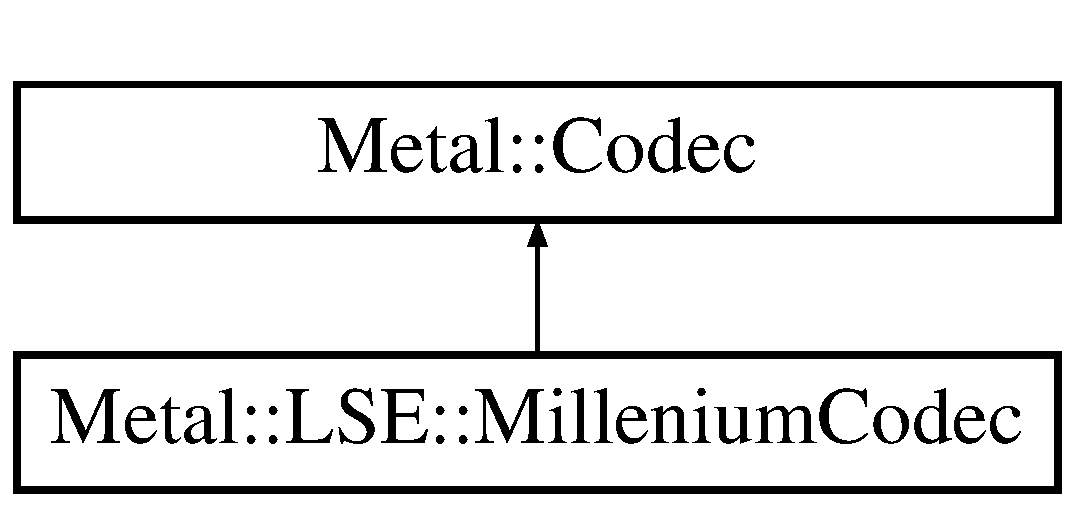
\includegraphics[height=2.000000cm]{classMetal_1_1LSE_1_1MilleniumCodec}
\end{center}
\end{figure}
\subsection*{Static Public Member Functions}
\begin{DoxyCompactItemize}
\item 
static void \hyperlink{classMetal_1_1LSE_1_1MilleniumCodec_a0db727988a60b489983d3650c2dbb5fd}{encode} (const \hyperlink{classMetal_1_1LSE_1_1OrderCancelRequest}{Order\+Cancel\+Request} \&ocr, \hyperlink{classMetal_1_1Message}{Message} \&msg)
\item 
static void \hyperlink{classMetal_1_1LSE_1_1MilleniumCodec_a90425eb0c5be795fb6c35fc28a88aac1}{encode} (const \hyperlink{classMetal_1_1LSE_1_1NewOrder}{New\+Order} \&no, \hyperlink{classMetal_1_1Message}{Message} \&msg)
\item 
static void \hyperlink{classMetal_1_1LSE_1_1MilleniumCodec_a2ae620b4b54cf5dc12df16b976af4d34}{encode} (const \hyperlink{classMetal_1_1LSE_1_1Logon}{Logon} \&logon, \hyperlink{classMetal_1_1Message}{Message} \&msg)
\item 
\hypertarget{classMetal_1_1LSE_1_1MilleniumCodec_a343c554002e86b3376c160ef5aa434d1}{}static void {\bfseries encode} (const int16\+\_\+t \&i, \hyperlink{classMetal_1_1Message}{Message} \&msg, int position)\label{classMetal_1_1LSE_1_1MilleniumCodec_a343c554002e86b3376c160ef5aa434d1}

\item 
\hypertarget{classMetal_1_1LSE_1_1MilleniumCodec_a7c950822487d09fde69d98224aa95442}{}static void {\bfseries encode} (const int32\+\_\+t \&i, \hyperlink{classMetal_1_1Message}{Message} \&msg, int position)\label{classMetal_1_1LSE_1_1MilleniumCodec_a7c950822487d09fde69d98224aa95442}

\item 
\hypertarget{classMetal_1_1LSE_1_1MilleniumCodec_a1b1d14237dd5a548b59a0a3773fbee79}{}static void {\bfseries encode} (const int64\+\_\+t \&i, \hyperlink{classMetal_1_1Message}{Message} \&msg, int position)\label{classMetal_1_1LSE_1_1MilleniumCodec_a1b1d14237dd5a548b59a0a3773fbee79}

\item 
\hypertarget{classMetal_1_1LSE_1_1MilleniumCodec_a3b494f4615faf56115c32db1c3fcf4c5}{}static void {\bfseries encode\+Header} (\hyperlink{classMetal_1_1Message}{Message} \&msg, int16\+\_\+t length, char type)\label{classMetal_1_1LSE_1_1MilleniumCodec_a3b494f4615faf56115c32db1c3fcf4c5}

\end{DoxyCompactItemize}


\subsection{Member Function Documentation}
\hypertarget{classMetal_1_1LSE_1_1MilleniumCodec_a0db727988a60b489983d3650c2dbb5fd}{}\index{Metal\+::\+L\+S\+E\+::\+Millenium\+Codec@{Metal\+::\+L\+S\+E\+::\+Millenium\+Codec}!encode@{encode}}
\index{encode@{encode}!Metal\+::\+L\+S\+E\+::\+Millenium\+Codec@{Metal\+::\+L\+S\+E\+::\+Millenium\+Codec}}
\subsubsection[{encode}]{\setlength{\rightskip}{0pt plus 5cm}void Metal\+::\+L\+S\+E\+::\+Millenium\+Codec\+::encode (
\begin{DoxyParamCaption}
\item[{const {\bf Order\+Cancel\+Request} \&}]{ocr, }
\item[{{\bf Metal\+::\+Message} \&}]{msg}
\end{DoxyParamCaption}
)\hspace{0.3cm}{\ttfamily [static]}}\label{classMetal_1_1LSE_1_1MilleniumCodec_a0db727988a60b489983d3650c2dbb5fd}
Encode a cancel request 
\begin{DoxyParams}{Parameters}
{\em ocr} & The Order Cancel Request representation \\
\hline
{\em msg} & The destination message \\
\hline
\end{DoxyParams}
\hypertarget{classMetal_1_1LSE_1_1MilleniumCodec_a90425eb0c5be795fb6c35fc28a88aac1}{}\index{Metal\+::\+L\+S\+E\+::\+Millenium\+Codec@{Metal\+::\+L\+S\+E\+::\+Millenium\+Codec}!encode@{encode}}
\index{encode@{encode}!Metal\+::\+L\+S\+E\+::\+Millenium\+Codec@{Metal\+::\+L\+S\+E\+::\+Millenium\+Codec}}
\subsubsection[{encode}]{\setlength{\rightskip}{0pt plus 5cm}void Metal\+::\+L\+S\+E\+::\+Millenium\+Codec\+::encode (
\begin{DoxyParamCaption}
\item[{const {\bf New\+Order} \&}]{no, }
\item[{{\bf Metal\+::\+Message} \&}]{msg}
\end{DoxyParamCaption}
)\hspace{0.3cm}{\ttfamily [static]}}\label{classMetal_1_1LSE_1_1MilleniumCodec_a90425eb0c5be795fb6c35fc28a88aac1}
Encode a new order 
\begin{DoxyParams}{Parameters}
{\em no} & The New Order representation \\
\hline
{\em msg} & The destination message \\
\hline
\end{DoxyParams}
\hypertarget{classMetal_1_1LSE_1_1MilleniumCodec_a2ae620b4b54cf5dc12df16b976af4d34}{}\index{Metal\+::\+L\+S\+E\+::\+Millenium\+Codec@{Metal\+::\+L\+S\+E\+::\+Millenium\+Codec}!encode@{encode}}
\index{encode@{encode}!Metal\+::\+L\+S\+E\+::\+Millenium\+Codec@{Metal\+::\+L\+S\+E\+::\+Millenium\+Codec}}
\subsubsection[{encode}]{\setlength{\rightskip}{0pt plus 5cm}void Metal\+::\+L\+S\+E\+::\+Millenium\+Codec\+::encode (
\begin{DoxyParamCaption}
\item[{const {\bf Logon} \&}]{logon, }
\item[{{\bf Metal\+::\+Message} \&}]{msg}
\end{DoxyParamCaption}
)\hspace{0.3cm}{\ttfamily [static]}}\label{classMetal_1_1LSE_1_1MilleniumCodec_a2ae620b4b54cf5dc12df16b976af4d34}
Encode a logon 
\begin{DoxyParams}{Parameters}
{\em logon} & \hyperlink{classMetal_1_1LSE_1_1Logon}{Logon} representation. Must be constructed with all values \\
\hline
{\em msg} & The destination message \\
\hline
\end{DoxyParams}


The documentation for this class was generated from the following files\+:\begin{DoxyCompactItemize}
\item 
/home/jc/metal/src/metal/adapters/\+L\+S\+E\+Trading\+Adapter/Millenium\+Codec.\+h\item 
/home/jc/metal/src/metal/adapters/\+L\+S\+E\+Trading\+Adapter/Millenium\+Codec.\+cpp\end{DoxyCompactItemize}

\hypertarget{classMetal_1_1LSE_1_1MilleniumMapper}{}\section{Metal\+:\+:L\+S\+E\+:\+:Millenium\+Mapper Class Reference}
\label{classMetal_1_1LSE_1_1MilleniumMapper}\index{Metal\+::\+L\+S\+E\+::\+Millenium\+Mapper@{Metal\+::\+L\+S\+E\+::\+Millenium\+Mapper}}
Inheritance diagram for Metal\+:\+:L\+S\+E\+:\+:Millenium\+Mapper\+:\begin{figure}[H]
\begin{center}
\leavevmode
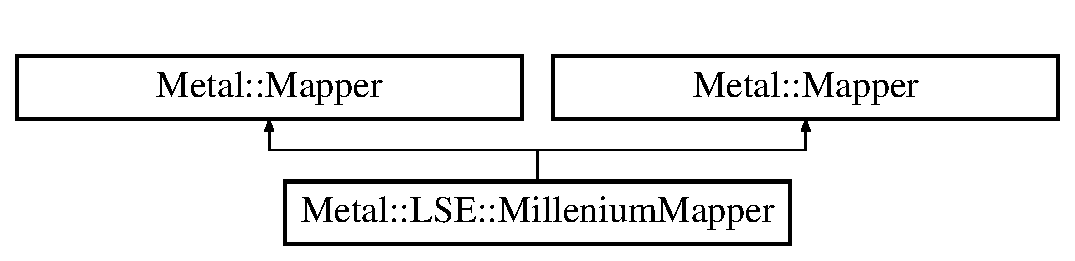
\includegraphics[height=2.000000cm]{classMetal_1_1LSE_1_1MilleniumMapper}
\end{center}
\end{figure}
\subsection*{Public Member Functions}
\begin{DoxyCompactItemize}
\item 
void \hyperlink{classMetal_1_1LSE_1_1MilleniumMapper_a63d9848ac2d8eb7c5e76e50c2d365c79}{benchmark} (std\+::vector$<$ \hyperlink{classMetal_1_1NewOrderSingle}{New\+Order\+Single} $>$ \&)
\end{DoxyCompactItemize}
\subsection*{Static Public Member Functions}
\begin{DoxyCompactItemize}
\item 
static void \hyperlink{classMetal_1_1LSE_1_1MilleniumMapper_a08f65c6357d8b450aff6335bf7dd4de8}{map} (const \hyperlink{classMetal_1_1LSE_1_1NewOrder}{New\+Order} \&, \hyperlink{classMetal_1_1NewOrderSingle}{New\+Order\+Single} \&)
\item 
static void \hyperlink{classMetal_1_1LSE_1_1MilleniumMapper_a83374c3bae042cd654f5f8b64d0584a2}{map} (const \hyperlink{classMetal_1_1NewOrderSingle}{New\+Order\+Single} \&, \hyperlink{classMetal_1_1LSE_1_1NewOrder}{New\+Order} \&)
\item 
static void \hyperlink{classMetal_1_1LSE_1_1MilleniumMapper_a21b4c1861b7c394ecae250baa685ab6d}{map} (const \hyperlink{classMetal_1_1OrderCancelRequest}{Metal\+::\+Order\+Cancel\+Request} \&, \hyperlink{classMetal_1_1LSE_1_1OrderCancelRequest}{Metal\+::\+L\+S\+E\+::\+Order\+Cancel\+Request} \&)
\item 
static void \hyperlink{classMetal_1_1LSE_1_1MilleniumMapper_a430f2f1f1f8dc53821e39ab90f6c78df}{map} (const F\+I\+X\+::\+Side \&, Metal\+::\+L\+S\+E\+::\+Side \&)
\end{DoxyCompactItemize}


\subsection{Member Function Documentation}
\hypertarget{classMetal_1_1LSE_1_1MilleniumMapper_a63d9848ac2d8eb7c5e76e50c2d365c79}{}\index{Metal\+::\+L\+S\+E\+::\+Millenium\+Mapper@{Metal\+::\+L\+S\+E\+::\+Millenium\+Mapper}!benchmark@{benchmark}}
\index{benchmark@{benchmark}!Metal\+::\+L\+S\+E\+::\+Millenium\+Mapper@{Metal\+::\+L\+S\+E\+::\+Millenium\+Mapper}}
\subsubsection[{benchmark}]{\setlength{\rightskip}{0pt plus 5cm}void Metal\+::\+L\+S\+E\+::\+Millenium\+Mapper\+::benchmark (
\begin{DoxyParamCaption}
\item[{std\+::vector$<$ {\bf New\+Order\+Single} $>$ \&}]{all\+Orders}
\end{DoxyParamCaption}
)}\label{classMetal_1_1LSE_1_1MilleniumMapper_a63d9848ac2d8eb7c5e76e50c2d365c79}
This is just a dumb loop that maps all incoming \hyperlink{classMetal_1_1NewOrderSingle}{New\+Order\+Single}. It has no other function than measuring mapping speed \hypertarget{classMetal_1_1LSE_1_1MilleniumMapper_a08f65c6357d8b450aff6335bf7dd4de8}{}\index{Metal\+::\+L\+S\+E\+::\+Millenium\+Mapper@{Metal\+::\+L\+S\+E\+::\+Millenium\+Mapper}!map@{map}}
\index{map@{map}!Metal\+::\+L\+S\+E\+::\+Millenium\+Mapper@{Metal\+::\+L\+S\+E\+::\+Millenium\+Mapper}}
\subsubsection[{map}]{\setlength{\rightskip}{0pt plus 5cm}void Metal\+::\+L\+S\+E\+::\+Millenium\+Mapper\+::map (
\begin{DoxyParamCaption}
\item[{const {\bf New\+Order} \&}]{message, }
\item[{{\bf New\+Order\+Single} \&}]{nos}
\end{DoxyParamCaption}
)\hspace{0.3cm}{\ttfamily [static]}}\label{classMetal_1_1LSE_1_1MilleniumMapper_a08f65c6357d8b450aff6335bf7dd4de8}
Translate L\+S\+E \hyperlink{classMetal_1_1LSE_1_1NewOrder}{New\+Order} into Metal representation \hypertarget{classMetal_1_1LSE_1_1MilleniumMapper_a83374c3bae042cd654f5f8b64d0584a2}{}\index{Metal\+::\+L\+S\+E\+::\+Millenium\+Mapper@{Metal\+::\+L\+S\+E\+::\+Millenium\+Mapper}!map@{map}}
\index{map@{map}!Metal\+::\+L\+S\+E\+::\+Millenium\+Mapper@{Metal\+::\+L\+S\+E\+::\+Millenium\+Mapper}}
\subsubsection[{map}]{\setlength{\rightskip}{0pt plus 5cm}void Metal\+::\+L\+S\+E\+::\+Millenium\+Mapper\+::map (
\begin{DoxyParamCaption}
\item[{const {\bf New\+Order\+Single} \&}]{nos, }
\item[{{\bf New\+Order} \&}]{new\+Order}
\end{DoxyParamCaption}
)\hspace{0.3cm}{\ttfamily [static]}}\label{classMetal_1_1LSE_1_1MilleniumMapper_a83374c3bae042cd654f5f8b64d0584a2}
Me\+T\+A\+L to L\+S\+E for \hyperlink{classMetal_1_1NewOrderSingle}{New\+Order\+Single}

\hyperlink{classMetal_1_1NewOrderSingle}{New\+Order\+Single} Me\+T\+A\+L -\/$>$ L\+S\+E 
\begin{DoxyExceptions}{Exceptions}
{\em F\+I\+X\+::\+Field\+Not\+Found} & \\
\hline
\end{DoxyExceptions}
\hypertarget{classMetal_1_1LSE_1_1MilleniumMapper_a21b4c1861b7c394ecae250baa685ab6d}{}\index{Metal\+::\+L\+S\+E\+::\+Millenium\+Mapper@{Metal\+::\+L\+S\+E\+::\+Millenium\+Mapper}!map@{map}}
\index{map@{map}!Metal\+::\+L\+S\+E\+::\+Millenium\+Mapper@{Metal\+::\+L\+S\+E\+::\+Millenium\+Mapper}}
\subsubsection[{map}]{\setlength{\rightskip}{0pt plus 5cm}void Metal\+::\+L\+S\+E\+::\+Millenium\+Mapper\+::map (
\begin{DoxyParamCaption}
\item[{const {\bf Metal\+::\+Order\+Cancel\+Request} \&}]{ocr\+From, }
\item[{{\bf Metal\+::\+L\+S\+E\+::\+Order\+Cancel\+Request} \&}]{ocr\+To}
\end{DoxyParamCaption}
)\hspace{0.3cm}{\ttfamily [static]}}\label{classMetal_1_1LSE_1_1MilleniumMapper_a21b4c1861b7c394ecae250baa685ab6d}
Me\+T\+A\+L to L\+S\+E for \hyperlink{classMetal_1_1LSE_1_1OrderCancelRequest}{Order\+Cancel\+Request}

Order\+Cancel Request Metal -\/$>$ L\+S\+E \hypertarget{classMetal_1_1LSE_1_1MilleniumMapper_a430f2f1f1f8dc53821e39ab90f6c78df}{}\index{Metal\+::\+L\+S\+E\+::\+Millenium\+Mapper@{Metal\+::\+L\+S\+E\+::\+Millenium\+Mapper}!map@{map}}
\index{map@{map}!Metal\+::\+L\+S\+E\+::\+Millenium\+Mapper@{Metal\+::\+L\+S\+E\+::\+Millenium\+Mapper}}
\subsubsection[{map}]{\setlength{\rightskip}{0pt plus 5cm}void Metal\+::\+L\+S\+E\+::\+Millenium\+Mapper\+::map (
\begin{DoxyParamCaption}
\item[{const F\+I\+X\+::\+Side \&}]{side\+From, }
\item[{Metal\+::\+L\+S\+E\+::\+Side \&}]{side\+To}
\end{DoxyParamCaption}
)\hspace{0.3cm}{\ttfamily [static]}}\label{classMetal_1_1LSE_1_1MilleniumMapper_a430f2f1f1f8dc53821e39ab90f6c78df}
Metal to L\+S\+E for Side

Side Metal -\/$>$ L\+S\+E 

The documentation for this class was generated from the following files\+:\begin{DoxyCompactItemize}
\item 
/home/jc/metal/src/metal/adapters/\+L\+S\+E\+Trading\+Adapter/Millenium\+Mapper.\+h\item 
/home/jc/metal/src/metal/adapters/\+L\+S\+E\+Trading\+Adapter/Millenium\+Mapper.\+cpp\end{DoxyCompactItemize}

\hypertarget{classMetal_1_1QuickFIX_1_1MyApplication}{}\section{Metal\+:\+:Quick\+F\+I\+X\+:\+:My\+Application Class Reference}
\label{classMetal_1_1QuickFIX_1_1MyApplication}\index{Metal\+::\+Quick\+F\+I\+X\+::\+My\+Application@{Metal\+::\+Quick\+F\+I\+X\+::\+My\+Application}}
Inheritance diagram for Metal\+:\+:Quick\+F\+I\+X\+:\+:My\+Application\+:\begin{figure}[H]
\begin{center}
\leavevmode
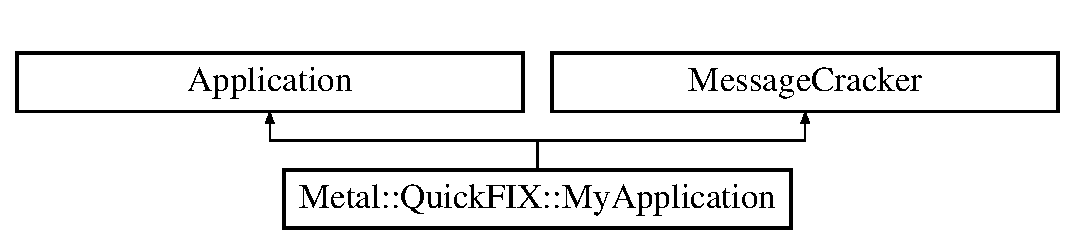
\includegraphics[height=2.000000cm]{classMetal_1_1QuickFIX_1_1MyApplication}
\end{center}
\end{figure}
\subsection*{Public Member Functions}
\begin{DoxyCompactItemize}
\item 
\hyperlink{classMetal_1_1QuickFIX_1_1MyApplication_ac015be7d9bb1677acda6fa464ce0f8ea}{My\+Application} (\hyperlink{classMetal_1_1QuickFIX_1_1QuickFIXAdapter}{Quick\+F\+I\+X\+Adapter} $\ast$pqfa)
\item 
\hyperlink{classMetal_1_1QuickFIX_1_1MyApplication_a1863c717971ba7a4d89dc50ee369abde}{$\sim$\+My\+Application} ()
\item 
void \hyperlink{classMetal_1_1QuickFIX_1_1MyApplication_a3f94210c4e0cbe060de70f7a875195c0}{on\+Create} (const Session\+I\+D \&)
\item 
void \hyperlink{classMetal_1_1QuickFIX_1_1MyApplication_a8dd2c71b6ec276e4f3da25d3b58710b8}{on\+Logon} (const Session\+I\+D \&)
\item 
void \hyperlink{classMetal_1_1QuickFIX_1_1MyApplication_ab5519b36c6fa527fd482bfb6864bad44}{on\+Logout} (const Session\+I\+D \&)
\item 
void \hyperlink{classMetal_1_1QuickFIX_1_1MyApplication_aa884521d47f50ff8c66c4ccd1409e1d6}{to\+Admin} (F\+I\+X\+::\+Message \&, const Session\+I\+D \&)
\item 
void \hyperlink{classMetal_1_1QuickFIX_1_1MyApplication_af32204a063c0a11009652626c86b24d0}{to\+App} (F\+I\+X\+::\+Message \&, const Session\+I\+D \&)  throw ( Do\+Not\+Send )
\item 
void \hyperlink{classMetal_1_1QuickFIX_1_1MyApplication_a4805e0aa8bc992043a2e3a0a4f818221}{from\+Admin} (const F\+I\+X\+::\+Message \&, const Session\+I\+D \&)  throw ( Field\+Not\+Found, Incorrect\+Data\+Format, Incorrect\+Tag\+Value, Reject\+Logon )
\item 
void \hyperlink{classMetal_1_1QuickFIX_1_1MyApplication_aca5ad6dbc249cb4093988887224598a6}{from\+App} (const F\+I\+X\+::\+Message \&message, const Session\+I\+D \&session\+I\+D)  throw ( Field\+Not\+Found, Incorrect\+Data\+Format, Incorrect\+Tag\+Value, Unsupported\+Message\+Type )
\item 
void \hyperlink{classMetal_1_1QuickFIX_1_1MyApplication_a6d513e282a19bbccd0719c39ca5c5dcf}{on\+Message} (const F\+I\+X42\+::\+Execution\+Report \&message, const Session\+I\+D \&)
\item 
void \hyperlink{classMetal_1_1QuickFIX_1_1MyApplication_a0bdc162c886f9aa87b481877d990a084}{on\+Message} (const F\+I\+X44\+::\+Execution\+Report \&message, const Session\+I\+D \&)
\end{DoxyCompactItemize}


\subsection{Constructor \& Destructor Documentation}
\hypertarget{classMetal_1_1QuickFIX_1_1MyApplication_ac015be7d9bb1677acda6fa464ce0f8ea}{}\index{Metal\+::\+Quick\+F\+I\+X\+::\+My\+Application@{Metal\+::\+Quick\+F\+I\+X\+::\+My\+Application}!My\+Application@{My\+Application}}
\index{My\+Application@{My\+Application}!Metal\+::\+Quick\+F\+I\+X\+::\+My\+Application@{Metal\+::\+Quick\+F\+I\+X\+::\+My\+Application}}
\subsubsection[{My\+Application}]{\setlength{\rightskip}{0pt plus 5cm}Metal\+::\+Quick\+F\+I\+X\+::\+My\+Application\+::\+My\+Application (
\begin{DoxyParamCaption}
\item[{{\bf Quick\+F\+I\+X\+Adapter} $\ast$}]{pqfa}
\end{DoxyParamCaption}
)\hspace{0.3cm}{\ttfamily [inline]}}\label{classMetal_1_1QuickFIX_1_1MyApplication_ac015be7d9bb1677acda6fa464ce0f8ea}
\hypertarget{classMetal_1_1QuickFIX_1_1MyApplication_a1863c717971ba7a4d89dc50ee369abde}{}\index{Metal\+::\+Quick\+F\+I\+X\+::\+My\+Application@{Metal\+::\+Quick\+F\+I\+X\+::\+My\+Application}!````~My\+Application@{$\sim$\+My\+Application}}
\index{````~My\+Application@{$\sim$\+My\+Application}!Metal\+::\+Quick\+F\+I\+X\+::\+My\+Application@{Metal\+::\+Quick\+F\+I\+X\+::\+My\+Application}}
\subsubsection[{$\sim$\+My\+Application}]{\setlength{\rightskip}{0pt plus 5cm}Metal\+::\+Quick\+F\+I\+X\+::\+My\+Application\+::$\sim$\+My\+Application (
\begin{DoxyParamCaption}
{}
\end{DoxyParamCaption}
)\hspace{0.3cm}{\ttfamily [inline]}}\label{classMetal_1_1QuickFIX_1_1MyApplication_a1863c717971ba7a4d89dc50ee369abde}


\subsection{Member Function Documentation}
\hypertarget{classMetal_1_1QuickFIX_1_1MyApplication_a4805e0aa8bc992043a2e3a0a4f818221}{}\index{Metal\+::\+Quick\+F\+I\+X\+::\+My\+Application@{Metal\+::\+Quick\+F\+I\+X\+::\+My\+Application}!from\+Admin@{from\+Admin}}
\index{from\+Admin@{from\+Admin}!Metal\+::\+Quick\+F\+I\+X\+::\+My\+Application@{Metal\+::\+Quick\+F\+I\+X\+::\+My\+Application}}
\subsubsection[{from\+Admin}]{\setlength{\rightskip}{0pt plus 5cm}void Metal\+::\+Quick\+F\+I\+X\+::\+My\+Application\+::from\+Admin (
\begin{DoxyParamCaption}
\item[{const F\+I\+X\+::\+Message \&}]{, }
\item[{const Session\+I\+D \&}]{}
\end{DoxyParamCaption}
) throw   Field\+Not\+Found,  Incorrect\+Data\+Format,  Incorrect\+Tag\+Value, Reject\+Logon) \hspace{0.3cm}{\ttfamily [inline]}}\label{classMetal_1_1QuickFIX_1_1MyApplication_a4805e0aa8bc992043a2e3a0a4f818221}
\hypertarget{classMetal_1_1QuickFIX_1_1MyApplication_aca5ad6dbc249cb4093988887224598a6}{}\index{Metal\+::\+Quick\+F\+I\+X\+::\+My\+Application@{Metal\+::\+Quick\+F\+I\+X\+::\+My\+Application}!from\+App@{from\+App}}
\index{from\+App@{from\+App}!Metal\+::\+Quick\+F\+I\+X\+::\+My\+Application@{Metal\+::\+Quick\+F\+I\+X\+::\+My\+Application}}
\subsubsection[{from\+App}]{\setlength{\rightskip}{0pt plus 5cm}void Metal\+::\+Quick\+F\+I\+X\+::\+My\+Application\+::from\+App (
\begin{DoxyParamCaption}
\item[{const F\+I\+X\+::\+Message \&}]{message, }
\item[{const Session\+I\+D \&}]{session\+I\+D}
\end{DoxyParamCaption}
) throw   Field\+Not\+Found,  Incorrect\+Data\+Format,  Incorrect\+Tag\+Value, Unsupported\+Message\+Type) \hspace{0.3cm}{\ttfamily [inline]}}\label{classMetal_1_1QuickFIX_1_1MyApplication_aca5ad6dbc249cb4093988887224598a6}
\hypertarget{classMetal_1_1QuickFIX_1_1MyApplication_a3f94210c4e0cbe060de70f7a875195c0}{}\index{Metal\+::\+Quick\+F\+I\+X\+::\+My\+Application@{Metal\+::\+Quick\+F\+I\+X\+::\+My\+Application}!on\+Create@{on\+Create}}
\index{on\+Create@{on\+Create}!Metal\+::\+Quick\+F\+I\+X\+::\+My\+Application@{Metal\+::\+Quick\+F\+I\+X\+::\+My\+Application}}
\subsubsection[{on\+Create}]{\setlength{\rightskip}{0pt plus 5cm}void Metal\+::\+Quick\+F\+I\+X\+::\+My\+Application\+::on\+Create (
\begin{DoxyParamCaption}
\item[{const Session\+I\+D \&}]{}
\end{DoxyParamCaption}
)\hspace{0.3cm}{\ttfamily [inline]}}\label{classMetal_1_1QuickFIX_1_1MyApplication_a3f94210c4e0cbe060de70f7a875195c0}
\hypertarget{classMetal_1_1QuickFIX_1_1MyApplication_a8dd2c71b6ec276e4f3da25d3b58710b8}{}\index{Metal\+::\+Quick\+F\+I\+X\+::\+My\+Application@{Metal\+::\+Quick\+F\+I\+X\+::\+My\+Application}!on\+Logon@{on\+Logon}}
\index{on\+Logon@{on\+Logon}!Metal\+::\+Quick\+F\+I\+X\+::\+My\+Application@{Metal\+::\+Quick\+F\+I\+X\+::\+My\+Application}}
\subsubsection[{on\+Logon}]{\setlength{\rightskip}{0pt plus 5cm}void Metal\+::\+Quick\+F\+I\+X\+::\+My\+Application\+::on\+Logon (
\begin{DoxyParamCaption}
\item[{const Session\+I\+D \&}]{}
\end{DoxyParamCaption}
)\hspace{0.3cm}{\ttfamily [inline]}}\label{classMetal_1_1QuickFIX_1_1MyApplication_a8dd2c71b6ec276e4f3da25d3b58710b8}
\hypertarget{classMetal_1_1QuickFIX_1_1MyApplication_ab5519b36c6fa527fd482bfb6864bad44}{}\index{Metal\+::\+Quick\+F\+I\+X\+::\+My\+Application@{Metal\+::\+Quick\+F\+I\+X\+::\+My\+Application}!on\+Logout@{on\+Logout}}
\index{on\+Logout@{on\+Logout}!Metal\+::\+Quick\+F\+I\+X\+::\+My\+Application@{Metal\+::\+Quick\+F\+I\+X\+::\+My\+Application}}
\subsubsection[{on\+Logout}]{\setlength{\rightskip}{0pt plus 5cm}void Metal\+::\+Quick\+F\+I\+X\+::\+My\+Application\+::on\+Logout (
\begin{DoxyParamCaption}
\item[{const Session\+I\+D \&}]{}
\end{DoxyParamCaption}
)\hspace{0.3cm}{\ttfamily [inline]}}\label{classMetal_1_1QuickFIX_1_1MyApplication_ab5519b36c6fa527fd482bfb6864bad44}
\hypertarget{classMetal_1_1QuickFIX_1_1MyApplication_a6d513e282a19bbccd0719c39ca5c5dcf}{}\index{Metal\+::\+Quick\+F\+I\+X\+::\+My\+Application@{Metal\+::\+Quick\+F\+I\+X\+::\+My\+Application}!on\+Message@{on\+Message}}
\index{on\+Message@{on\+Message}!Metal\+::\+Quick\+F\+I\+X\+::\+My\+Application@{Metal\+::\+Quick\+F\+I\+X\+::\+My\+Application}}
\subsubsection[{on\+Message}]{\setlength{\rightskip}{0pt plus 5cm}void Metal\+::\+Quick\+F\+I\+X\+::\+My\+Application\+::on\+Message (
\begin{DoxyParamCaption}
\item[{const F\+I\+X42\+::\+Execution\+Report \&}]{message, }
\item[{const Session\+I\+D \&}]{}
\end{DoxyParamCaption}
)\hspace{0.3cm}{\ttfamily [inline]}}\label{classMetal_1_1QuickFIX_1_1MyApplication_a6d513e282a19bbccd0719c39ca5c5dcf}
\hypertarget{classMetal_1_1QuickFIX_1_1MyApplication_a0bdc162c886f9aa87b481877d990a084}{}\index{Metal\+::\+Quick\+F\+I\+X\+::\+My\+Application@{Metal\+::\+Quick\+F\+I\+X\+::\+My\+Application}!on\+Message@{on\+Message}}
\index{on\+Message@{on\+Message}!Metal\+::\+Quick\+F\+I\+X\+::\+My\+Application@{Metal\+::\+Quick\+F\+I\+X\+::\+My\+Application}}
\subsubsection[{on\+Message}]{\setlength{\rightskip}{0pt plus 5cm}void Metal\+::\+Quick\+F\+I\+X\+::\+My\+Application\+::on\+Message (
\begin{DoxyParamCaption}
\item[{const F\+I\+X44\+::\+Execution\+Report \&}]{message, }
\item[{const Session\+I\+D \&}]{}
\end{DoxyParamCaption}
)\hspace{0.3cm}{\ttfamily [inline]}}\label{classMetal_1_1QuickFIX_1_1MyApplication_a0bdc162c886f9aa87b481877d990a084}
\hypertarget{classMetal_1_1QuickFIX_1_1MyApplication_aa884521d47f50ff8c66c4ccd1409e1d6}{}\index{Metal\+::\+Quick\+F\+I\+X\+::\+My\+Application@{Metal\+::\+Quick\+F\+I\+X\+::\+My\+Application}!to\+Admin@{to\+Admin}}
\index{to\+Admin@{to\+Admin}!Metal\+::\+Quick\+F\+I\+X\+::\+My\+Application@{Metal\+::\+Quick\+F\+I\+X\+::\+My\+Application}}
\subsubsection[{to\+Admin}]{\setlength{\rightskip}{0pt plus 5cm}void Metal\+::\+Quick\+F\+I\+X\+::\+My\+Application\+::to\+Admin (
\begin{DoxyParamCaption}
\item[{F\+I\+X\+::\+Message \&}]{, }
\item[{const Session\+I\+D \&}]{}
\end{DoxyParamCaption}
)\hspace{0.3cm}{\ttfamily [inline]}}\label{classMetal_1_1QuickFIX_1_1MyApplication_aa884521d47f50ff8c66c4ccd1409e1d6}
\hypertarget{classMetal_1_1QuickFIX_1_1MyApplication_af32204a063c0a11009652626c86b24d0}{}\index{Metal\+::\+Quick\+F\+I\+X\+::\+My\+Application@{Metal\+::\+Quick\+F\+I\+X\+::\+My\+Application}!to\+App@{to\+App}}
\index{to\+App@{to\+App}!Metal\+::\+Quick\+F\+I\+X\+::\+My\+Application@{Metal\+::\+Quick\+F\+I\+X\+::\+My\+Application}}
\subsubsection[{to\+App}]{\setlength{\rightskip}{0pt plus 5cm}void Metal\+::\+Quick\+F\+I\+X\+::\+My\+Application\+::to\+App (
\begin{DoxyParamCaption}
\item[{F\+I\+X\+::\+Message \&}]{, }
\item[{const Session\+I\+D \&}]{}
\end{DoxyParamCaption}
) throw  Do\+Not\+Send) \hspace{0.3cm}{\ttfamily [inline]}}\label{classMetal_1_1QuickFIX_1_1MyApplication_af32204a063c0a11009652626c86b24d0}


The documentation for this class was generated from the following file\+:\begin{DoxyCompactItemize}
\item 
/home/jc/metal/github/src/adapters/\+Quick\+F\+I\+X\+Adapter/\hyperlink{QuickFIXAdapter_8cpp}{Quick\+F\+I\+X\+Adapter.\+cpp}\end{DoxyCompactItemize}

\hypertarget{classMetal_1_1LSE_1_1NewOrder}{}\section{Metal\+:\+:L\+S\+E\+:\+:New\+Order Class Reference}
\label{classMetal_1_1LSE_1_1NewOrder}\index{Metal\+::\+L\+S\+E\+::\+New\+Order@{Metal\+::\+L\+S\+E\+::\+New\+Order}}


{\ttfamily \#include $<$New\+Order.\+h$>$}

\subsection*{Public Member Functions}
\begin{DoxyCompactItemize}
\item 
\hyperlink{classMetal_1_1LSE_1_1NewOrder_aeaedaf6e5ebd46fbb1448b95c2791dcd}{New\+Order} ()
\item 
virtual \hyperlink{classMetal_1_1LSE_1_1NewOrder_acf2c36880aedda0edef97616a8d002fd}{$\sim$\+New\+Order} ()
\end{DoxyCompactItemize}
\subsection*{Public Attributes}
\begin{DoxyCompactItemize}
\item 
std\+::string \hyperlink{classMetal_1_1LSE_1_1NewOrder_a53ce2b8f89f168c58fa2a8f97ce79c93}{client\+Order\+I\+D}
\item 
std\+::string \hyperlink{classMetal_1_1LSE_1_1NewOrder_aff72605e8542180dad099904873bda84}{trader\+I\+D}
\item 
std\+::string \hyperlink{classMetal_1_1LSE_1_1NewOrder_a80ad2239737f52a61a27eb4f6193bdba}{account}
\item 
\hyperlink{namespaceMetal_1_1LSE_ae1f2b67d6be84798adfd29525ee0a697}{Clearing\+Acount} \hyperlink{classMetal_1_1LSE_1_1NewOrder_a65522450bdc6e5ac29e739738bbba34e}{clearing\+Account}
\item 
\hyperlink{namespaceMetal_1_1LSE_a5280aa41aaa4433df351e733a23ecd14}{Instrument\+I\+D} \hyperlink{classMetal_1_1LSE_1_1NewOrder_aeffc76c3cb37c6bd7f6e2a9c5fa4d441}{instrument\+I\+D}
\item 
\hyperlink{namespaceMetal_1_1LSE_aff01f13ff9de4cacdd0436f6956df4fb}{Order\+Type} \hyperlink{classMetal_1_1LSE_1_1NewOrder_aca679f638141bbae5505ed8bb6961378}{order\+Type}
\item 
\hyperlink{namespaceMetal_1_1LSE_a59a4a742606e572af3f14a34a7503ee9}{Time\+In\+Force} \hyperlink{classMetal_1_1LSE_1_1NewOrder_ab0da192ab665eeffa7797f901d2f94fc}{time\+In\+Force}
\item 
\hyperlink{namespaceMetal_1_1LSE_a62b04587ecad5f88a7fbd626194b3c28}{Expire\+Date\+Time} \hyperlink{classMetal_1_1LSE_1_1NewOrder_a75f27f7515b6214b615681e5fc5074c3}{expire\+Date\+Time}
\item 
\hyperlink{namespaceMetal_1_1LSE_af5236b7a999484d8cd5b579b7d7c133b}{Side} \hyperlink{classMetal_1_1LSE_1_1NewOrder_ac13fa3b75b0b41ee60fb6fcf3b57fb31}{side}
\item 
\hyperlink{namespaceMetal_1_1LSE_a86342859fb8034a9649f6d789e97d9da}{Quantity} \hyperlink{classMetal_1_1LSE_1_1NewOrder_a79d35c9c9c65c2acded727062c1b70bd}{order\+Qty}
\item 
\hyperlink{namespaceMetal_1_1LSE_a86342859fb8034a9649f6d789e97d9da}{Quantity} \hyperlink{classMetal_1_1LSE_1_1NewOrder_a7cae6ab56cd3c9a8f973005f0aaaf27e}{display\+Qty}
\item 
\hyperlink{namespaceMetal_1_1LSE_a4a629b5e2aed21d653db0debf8b63af4}{Price} \hyperlink{classMetal_1_1LSE_1_1NewOrder_acff28c03d42db0449f23f480be72c3a9}{limit\+Price}
\item 
\hyperlink{namespaceMetal_1_1LSE_aff7400475e278748e213fefa47bb9b99}{Capacity} \hyperlink{classMetal_1_1LSE_1_1NewOrder_aeace92cd76c0bb8539f82fdfff170115}{capacity}
\item 
\hyperlink{namespaceMetal_1_1LSE_a28e46ba33ca9d641a9ea0c63a2e35141}{Auto\+Cancel} \hyperlink{classMetal_1_1LSE_1_1NewOrder_aacc7198bc8dee4a9bf98bd8bc13dc85b}{auto\+Cancel}
\item 
\hyperlink{namespaceMetal_1_1LSE_afd57250a16de7395f5ad2bc63c7b8e5e}{Order\+Sub\+Type} \hyperlink{classMetal_1_1LSE_1_1NewOrder_a11797541566225395362ff7f9c0e3557}{order\+Sub\+Type}
\item 
\hyperlink{namespaceMetal_1_1LSE_a0c110efde74bd7f4315615c477dac047}{Anonymity} \hyperlink{classMetal_1_1LSE_1_1NewOrder_ab9c132be0c599c5d113d20603bb6f19d}{anonymity}
\item 
\hyperlink{namespaceMetal_1_1LSE_a4a629b5e2aed21d653db0debf8b63af4}{Price} \hyperlink{classMetal_1_1LSE_1_1NewOrder_abf0f20401650effe0dba393616128d0b}{stopped\+Price}
\item 
\hyperlink{namespaceMetal_1_1LSE_afb7bdec752b9048b6d725e2421586a64}{Passive\+Only\+Order} \hyperlink{classMetal_1_1LSE_1_1NewOrder_a4debc1666c97f2c3127ed05fe9373856}{passive\+Only\+Order}
\end{DoxyCompactItemize}
\subsection*{Static Public Attributes}
\begin{DoxyCompactItemize}
\item 
static const int \hyperlink{classMetal_1_1LSE_1_1NewOrder_a1b9c8980a62d9902914b215a139740ba}{S\+I\+Z\+E} = 97
\end{DoxyCompactItemize}


\subsection{Constructor \& Destructor Documentation}
\hypertarget{classMetal_1_1LSE_1_1NewOrder_aeaedaf6e5ebd46fbb1448b95c2791dcd}{}\index{Metal\+::\+L\+S\+E\+::\+New\+Order@{Metal\+::\+L\+S\+E\+::\+New\+Order}!New\+Order@{New\+Order}}
\index{New\+Order@{New\+Order}!Metal\+::\+L\+S\+E\+::\+New\+Order@{Metal\+::\+L\+S\+E\+::\+New\+Order}}
\subsubsection[{New\+Order}]{\setlength{\rightskip}{0pt plus 5cm}Metal\+::\+L\+S\+E\+::\+New\+Order\+::\+New\+Order (
\begin{DoxyParamCaption}
{}
\end{DoxyParamCaption}
)}\label{classMetal_1_1LSE_1_1NewOrder_aeaedaf6e5ebd46fbb1448b95c2791dcd}
\hypertarget{classMetal_1_1LSE_1_1NewOrder_acf2c36880aedda0edef97616a8d002fd}{}\index{Metal\+::\+L\+S\+E\+::\+New\+Order@{Metal\+::\+L\+S\+E\+::\+New\+Order}!````~New\+Order@{$\sim$\+New\+Order}}
\index{````~New\+Order@{$\sim$\+New\+Order}!Metal\+::\+L\+S\+E\+::\+New\+Order@{Metal\+::\+L\+S\+E\+::\+New\+Order}}
\subsubsection[{$\sim$\+New\+Order}]{\setlength{\rightskip}{0pt plus 5cm}Metal\+::\+L\+S\+E\+::\+New\+Order\+::$\sim$\+New\+Order (
\begin{DoxyParamCaption}
{}
\end{DoxyParamCaption}
)\hspace{0.3cm}{\ttfamily [virtual]}}\label{classMetal_1_1LSE_1_1NewOrder_acf2c36880aedda0edef97616a8d002fd}


\subsection{Member Data Documentation}
\hypertarget{classMetal_1_1LSE_1_1NewOrder_a80ad2239737f52a61a27eb4f6193bdba}{}\index{Metal\+::\+L\+S\+E\+::\+New\+Order@{Metal\+::\+L\+S\+E\+::\+New\+Order}!account@{account}}
\index{account@{account}!Metal\+::\+L\+S\+E\+::\+New\+Order@{Metal\+::\+L\+S\+E\+::\+New\+Order}}
\subsubsection[{account}]{\setlength{\rightskip}{0pt plus 5cm}std\+::string Metal\+::\+L\+S\+E\+::\+New\+Order\+::account}\label{classMetal_1_1LSE_1_1NewOrder_a80ad2239737f52a61a27eb4f6193bdba}
\hypertarget{classMetal_1_1LSE_1_1NewOrder_ab9c132be0c599c5d113d20603bb6f19d}{}\index{Metal\+::\+L\+S\+E\+::\+New\+Order@{Metal\+::\+L\+S\+E\+::\+New\+Order}!anonymity@{anonymity}}
\index{anonymity@{anonymity}!Metal\+::\+L\+S\+E\+::\+New\+Order@{Metal\+::\+L\+S\+E\+::\+New\+Order}}
\subsubsection[{anonymity}]{\setlength{\rightskip}{0pt plus 5cm}{\bf Anonymity} Metal\+::\+L\+S\+E\+::\+New\+Order\+::anonymity}\label{classMetal_1_1LSE_1_1NewOrder_ab9c132be0c599c5d113d20603bb6f19d}
\hypertarget{classMetal_1_1LSE_1_1NewOrder_aacc7198bc8dee4a9bf98bd8bc13dc85b}{}\index{Metal\+::\+L\+S\+E\+::\+New\+Order@{Metal\+::\+L\+S\+E\+::\+New\+Order}!auto\+Cancel@{auto\+Cancel}}
\index{auto\+Cancel@{auto\+Cancel}!Metal\+::\+L\+S\+E\+::\+New\+Order@{Metal\+::\+L\+S\+E\+::\+New\+Order}}
\subsubsection[{auto\+Cancel}]{\setlength{\rightskip}{0pt plus 5cm}{\bf Auto\+Cancel} Metal\+::\+L\+S\+E\+::\+New\+Order\+::auto\+Cancel}\label{classMetal_1_1LSE_1_1NewOrder_aacc7198bc8dee4a9bf98bd8bc13dc85b}
\hypertarget{classMetal_1_1LSE_1_1NewOrder_aeace92cd76c0bb8539f82fdfff170115}{}\index{Metal\+::\+L\+S\+E\+::\+New\+Order@{Metal\+::\+L\+S\+E\+::\+New\+Order}!capacity@{capacity}}
\index{capacity@{capacity}!Metal\+::\+L\+S\+E\+::\+New\+Order@{Metal\+::\+L\+S\+E\+::\+New\+Order}}
\subsubsection[{capacity}]{\setlength{\rightskip}{0pt plus 5cm}{\bf Capacity} Metal\+::\+L\+S\+E\+::\+New\+Order\+::capacity}\label{classMetal_1_1LSE_1_1NewOrder_aeace92cd76c0bb8539f82fdfff170115}
\hypertarget{classMetal_1_1LSE_1_1NewOrder_a65522450bdc6e5ac29e739738bbba34e}{}\index{Metal\+::\+L\+S\+E\+::\+New\+Order@{Metal\+::\+L\+S\+E\+::\+New\+Order}!clearing\+Account@{clearing\+Account}}
\index{clearing\+Account@{clearing\+Account}!Metal\+::\+L\+S\+E\+::\+New\+Order@{Metal\+::\+L\+S\+E\+::\+New\+Order}}
\subsubsection[{clearing\+Account}]{\setlength{\rightskip}{0pt plus 5cm}{\bf Clearing\+Acount} Metal\+::\+L\+S\+E\+::\+New\+Order\+::clearing\+Account}\label{classMetal_1_1LSE_1_1NewOrder_a65522450bdc6e5ac29e739738bbba34e}
\hypertarget{classMetal_1_1LSE_1_1NewOrder_a53ce2b8f89f168c58fa2a8f97ce79c93}{}\index{Metal\+::\+L\+S\+E\+::\+New\+Order@{Metal\+::\+L\+S\+E\+::\+New\+Order}!client\+Order\+I\+D@{client\+Order\+I\+D}}
\index{client\+Order\+I\+D@{client\+Order\+I\+D}!Metal\+::\+L\+S\+E\+::\+New\+Order@{Metal\+::\+L\+S\+E\+::\+New\+Order}}
\subsubsection[{client\+Order\+I\+D}]{\setlength{\rightskip}{0pt plus 5cm}std\+::string Metal\+::\+L\+S\+E\+::\+New\+Order\+::client\+Order\+I\+D}\label{classMetal_1_1LSE_1_1NewOrder_a53ce2b8f89f168c58fa2a8f97ce79c93}
\hypertarget{classMetal_1_1LSE_1_1NewOrder_a7cae6ab56cd3c9a8f973005f0aaaf27e}{}\index{Metal\+::\+L\+S\+E\+::\+New\+Order@{Metal\+::\+L\+S\+E\+::\+New\+Order}!display\+Qty@{display\+Qty}}
\index{display\+Qty@{display\+Qty}!Metal\+::\+L\+S\+E\+::\+New\+Order@{Metal\+::\+L\+S\+E\+::\+New\+Order}}
\subsubsection[{display\+Qty}]{\setlength{\rightskip}{0pt plus 5cm}{\bf Quantity} Metal\+::\+L\+S\+E\+::\+New\+Order\+::display\+Qty}\label{classMetal_1_1LSE_1_1NewOrder_a7cae6ab56cd3c9a8f973005f0aaaf27e}
\hypertarget{classMetal_1_1LSE_1_1NewOrder_a75f27f7515b6214b615681e5fc5074c3}{}\index{Metal\+::\+L\+S\+E\+::\+New\+Order@{Metal\+::\+L\+S\+E\+::\+New\+Order}!expire\+Date\+Time@{expire\+Date\+Time}}
\index{expire\+Date\+Time@{expire\+Date\+Time}!Metal\+::\+L\+S\+E\+::\+New\+Order@{Metal\+::\+L\+S\+E\+::\+New\+Order}}
\subsubsection[{expire\+Date\+Time}]{\setlength{\rightskip}{0pt plus 5cm}{\bf Expire\+Date\+Time} Metal\+::\+L\+S\+E\+::\+New\+Order\+::expire\+Date\+Time}\label{classMetal_1_1LSE_1_1NewOrder_a75f27f7515b6214b615681e5fc5074c3}
\hypertarget{classMetal_1_1LSE_1_1NewOrder_aeffc76c3cb37c6bd7f6e2a9c5fa4d441}{}\index{Metal\+::\+L\+S\+E\+::\+New\+Order@{Metal\+::\+L\+S\+E\+::\+New\+Order}!instrument\+I\+D@{instrument\+I\+D}}
\index{instrument\+I\+D@{instrument\+I\+D}!Metal\+::\+L\+S\+E\+::\+New\+Order@{Metal\+::\+L\+S\+E\+::\+New\+Order}}
\subsubsection[{instrument\+I\+D}]{\setlength{\rightskip}{0pt plus 5cm}{\bf Instrument\+I\+D} Metal\+::\+L\+S\+E\+::\+New\+Order\+::instrument\+I\+D}\label{classMetal_1_1LSE_1_1NewOrder_aeffc76c3cb37c6bd7f6e2a9c5fa4d441}
\hypertarget{classMetal_1_1LSE_1_1NewOrder_acff28c03d42db0449f23f480be72c3a9}{}\index{Metal\+::\+L\+S\+E\+::\+New\+Order@{Metal\+::\+L\+S\+E\+::\+New\+Order}!limit\+Price@{limit\+Price}}
\index{limit\+Price@{limit\+Price}!Metal\+::\+L\+S\+E\+::\+New\+Order@{Metal\+::\+L\+S\+E\+::\+New\+Order}}
\subsubsection[{limit\+Price}]{\setlength{\rightskip}{0pt plus 5cm}{\bf Price} Metal\+::\+L\+S\+E\+::\+New\+Order\+::limit\+Price}\label{classMetal_1_1LSE_1_1NewOrder_acff28c03d42db0449f23f480be72c3a9}
Price is stored with 8 implied decimal places \hypertarget{classMetal_1_1LSE_1_1NewOrder_a79d35c9c9c65c2acded727062c1b70bd}{}\index{Metal\+::\+L\+S\+E\+::\+New\+Order@{Metal\+::\+L\+S\+E\+::\+New\+Order}!order\+Qty@{order\+Qty}}
\index{order\+Qty@{order\+Qty}!Metal\+::\+L\+S\+E\+::\+New\+Order@{Metal\+::\+L\+S\+E\+::\+New\+Order}}
\subsubsection[{order\+Qty}]{\setlength{\rightskip}{0pt plus 5cm}{\bf Quantity} Metal\+::\+L\+S\+E\+::\+New\+Order\+::order\+Qty}\label{classMetal_1_1LSE_1_1NewOrder_a79d35c9c9c65c2acded727062c1b70bd}
\hypertarget{classMetal_1_1LSE_1_1NewOrder_a11797541566225395362ff7f9c0e3557}{}\index{Metal\+::\+L\+S\+E\+::\+New\+Order@{Metal\+::\+L\+S\+E\+::\+New\+Order}!order\+Sub\+Type@{order\+Sub\+Type}}
\index{order\+Sub\+Type@{order\+Sub\+Type}!Metal\+::\+L\+S\+E\+::\+New\+Order@{Metal\+::\+L\+S\+E\+::\+New\+Order}}
\subsubsection[{order\+Sub\+Type}]{\setlength{\rightskip}{0pt plus 5cm}{\bf Order\+Sub\+Type} Metal\+::\+L\+S\+E\+::\+New\+Order\+::order\+Sub\+Type}\label{classMetal_1_1LSE_1_1NewOrder_a11797541566225395362ff7f9c0e3557}
\hypertarget{classMetal_1_1LSE_1_1NewOrder_aca679f638141bbae5505ed8bb6961378}{}\index{Metal\+::\+L\+S\+E\+::\+New\+Order@{Metal\+::\+L\+S\+E\+::\+New\+Order}!order\+Type@{order\+Type}}
\index{order\+Type@{order\+Type}!Metal\+::\+L\+S\+E\+::\+New\+Order@{Metal\+::\+L\+S\+E\+::\+New\+Order}}
\subsubsection[{order\+Type}]{\setlength{\rightskip}{0pt plus 5cm}{\bf Order\+Type} Metal\+::\+L\+S\+E\+::\+New\+Order\+::order\+Type}\label{classMetal_1_1LSE_1_1NewOrder_aca679f638141bbae5505ed8bb6961378}
\hypertarget{classMetal_1_1LSE_1_1NewOrder_a4debc1666c97f2c3127ed05fe9373856}{}\index{Metal\+::\+L\+S\+E\+::\+New\+Order@{Metal\+::\+L\+S\+E\+::\+New\+Order}!passive\+Only\+Order@{passive\+Only\+Order}}
\index{passive\+Only\+Order@{passive\+Only\+Order}!Metal\+::\+L\+S\+E\+::\+New\+Order@{Metal\+::\+L\+S\+E\+::\+New\+Order}}
\subsubsection[{passive\+Only\+Order}]{\setlength{\rightskip}{0pt plus 5cm}{\bf Passive\+Only\+Order} Metal\+::\+L\+S\+E\+::\+New\+Order\+::passive\+Only\+Order}\label{classMetal_1_1LSE_1_1NewOrder_a4debc1666c97f2c3127ed05fe9373856}
\hypertarget{classMetal_1_1LSE_1_1NewOrder_ac13fa3b75b0b41ee60fb6fcf3b57fb31}{}\index{Metal\+::\+L\+S\+E\+::\+New\+Order@{Metal\+::\+L\+S\+E\+::\+New\+Order}!side@{side}}
\index{side@{side}!Metal\+::\+L\+S\+E\+::\+New\+Order@{Metal\+::\+L\+S\+E\+::\+New\+Order}}
\subsubsection[{side}]{\setlength{\rightskip}{0pt plus 5cm}{\bf Side} Metal\+::\+L\+S\+E\+::\+New\+Order\+::side}\label{classMetal_1_1LSE_1_1NewOrder_ac13fa3b75b0b41ee60fb6fcf3b57fb31}
\hypertarget{classMetal_1_1LSE_1_1NewOrder_a1b9c8980a62d9902914b215a139740ba}{}\index{Metal\+::\+L\+S\+E\+::\+New\+Order@{Metal\+::\+L\+S\+E\+::\+New\+Order}!S\+I\+Z\+E@{S\+I\+Z\+E}}
\index{S\+I\+Z\+E@{S\+I\+Z\+E}!Metal\+::\+L\+S\+E\+::\+New\+Order@{Metal\+::\+L\+S\+E\+::\+New\+Order}}
\subsubsection[{S\+I\+Z\+E}]{\setlength{\rightskip}{0pt plus 5cm}const int Metal\+::\+L\+S\+E\+::\+New\+Order\+::\+S\+I\+Z\+E = 97\hspace{0.3cm}{\ttfamily [static]}}\label{classMetal_1_1LSE_1_1NewOrder_a1b9c8980a62d9902914b215a139740ba}
\hypertarget{classMetal_1_1LSE_1_1NewOrder_abf0f20401650effe0dba393616128d0b}{}\index{Metal\+::\+L\+S\+E\+::\+New\+Order@{Metal\+::\+L\+S\+E\+::\+New\+Order}!stopped\+Price@{stopped\+Price}}
\index{stopped\+Price@{stopped\+Price}!Metal\+::\+L\+S\+E\+::\+New\+Order@{Metal\+::\+L\+S\+E\+::\+New\+Order}}
\subsubsection[{stopped\+Price}]{\setlength{\rightskip}{0pt plus 5cm}{\bf Price} Metal\+::\+L\+S\+E\+::\+New\+Order\+::stopped\+Price}\label{classMetal_1_1LSE_1_1NewOrder_abf0f20401650effe0dba393616128d0b}
\hypertarget{classMetal_1_1LSE_1_1NewOrder_ab0da192ab665eeffa7797f901d2f94fc}{}\index{Metal\+::\+L\+S\+E\+::\+New\+Order@{Metal\+::\+L\+S\+E\+::\+New\+Order}!time\+In\+Force@{time\+In\+Force}}
\index{time\+In\+Force@{time\+In\+Force}!Metal\+::\+L\+S\+E\+::\+New\+Order@{Metal\+::\+L\+S\+E\+::\+New\+Order}}
\subsubsection[{time\+In\+Force}]{\setlength{\rightskip}{0pt plus 5cm}{\bf Time\+In\+Force} Metal\+::\+L\+S\+E\+::\+New\+Order\+::time\+In\+Force}\label{classMetal_1_1LSE_1_1NewOrder_ab0da192ab665eeffa7797f901d2f94fc}
\hypertarget{classMetal_1_1LSE_1_1NewOrder_aff72605e8542180dad099904873bda84}{}\index{Metal\+::\+L\+S\+E\+::\+New\+Order@{Metal\+::\+L\+S\+E\+::\+New\+Order}!trader\+I\+D@{trader\+I\+D}}
\index{trader\+I\+D@{trader\+I\+D}!Metal\+::\+L\+S\+E\+::\+New\+Order@{Metal\+::\+L\+S\+E\+::\+New\+Order}}
\subsubsection[{trader\+I\+D}]{\setlength{\rightskip}{0pt plus 5cm}std\+::string Metal\+::\+L\+S\+E\+::\+New\+Order\+::trader\+I\+D}\label{classMetal_1_1LSE_1_1NewOrder_aff72605e8542180dad099904873bda84}


The documentation for this class was generated from the following files\+:\begin{DoxyCompactItemize}
\item 
/home/jc/metal/github/src/adapters/\+L\+S\+E\+Trading\+Adapter/\hyperlink{NewOrder_8h}{New\+Order.\+h}\item 
/home/jc/metal/github/src/adapters/\+L\+S\+E\+Trading\+Adapter/\hyperlink{NewOrder_8cpp}{New\+Order.\+cpp}\end{DoxyCompactItemize}

\hypertarget{classMetal_1_1NewOrderSingle}{}\section{Metal\+:\+:New\+Order\+Single Class Reference}
\label{classMetal_1_1NewOrderSingle}\index{Metal\+::\+New\+Order\+Single@{Metal\+::\+New\+Order\+Single}}
Inheritance diagram for Metal\+:\+:New\+Order\+Single\+:\begin{figure}[H]
\begin{center}
\leavevmode
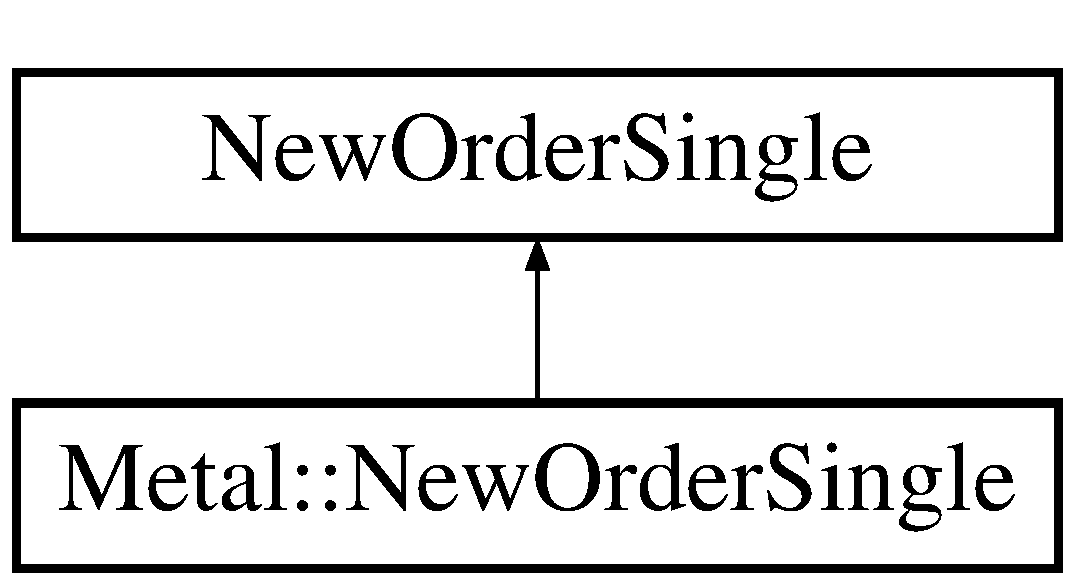
\includegraphics[height=2.000000cm]{classMetal_1_1NewOrderSingle}
\end{center}
\end{figure}


The documentation for this class was generated from the following file\+:\begin{DoxyCompactItemize}
\item 
/home/jc/metal/src/metal/metal.\+h\end{DoxyCompactItemize}

\hypertarget{classOnAccept}{}\section{On\+Accept Class Reference}
\label{classOnAccept}\index{On\+Accept@{On\+Accept}}
Inheritance diagram for On\+Accept\+:\begin{figure}[H]
\begin{center}
\leavevmode
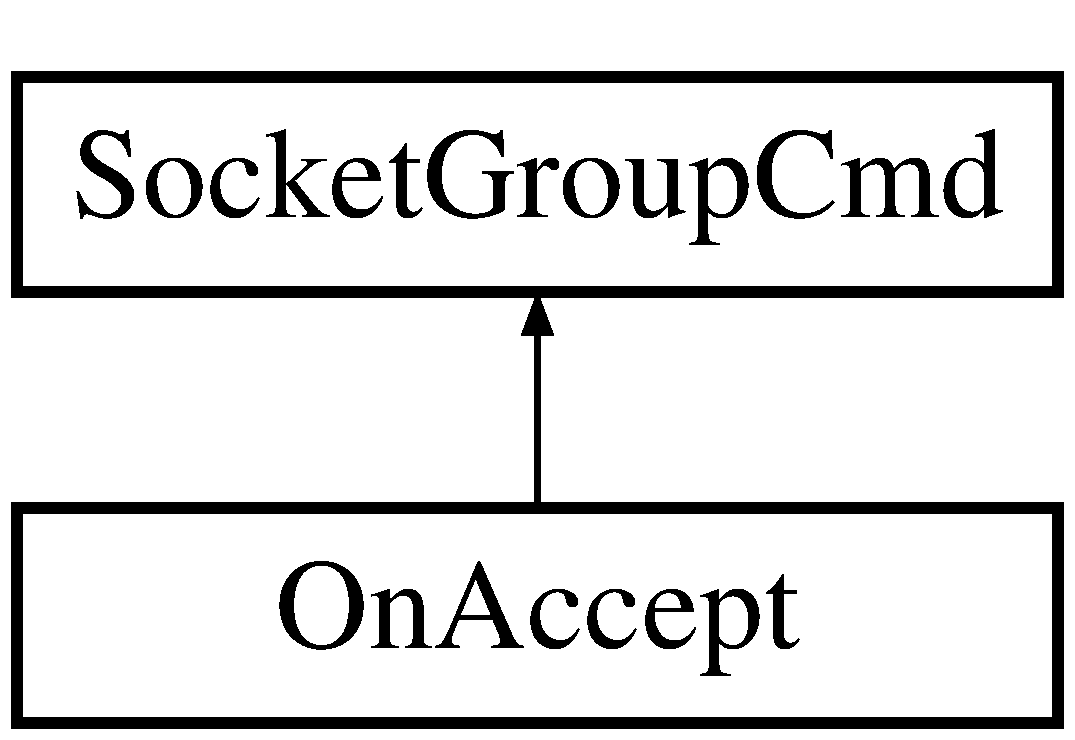
\includegraphics[height=2.000000cm]{classOnAccept}
\end{center}
\end{figure}


The documentation for this class was generated from the following file\+:\begin{DoxyCompactItemize}
\item 
/home/jc/metal/github/src/3rdparties/net\+Link/examples/socket\+\_\+group/\hyperlink{chatServer_8cc}{chat\+Server.\+cc}\end{DoxyCompactItemize}

\hypertarget{classOnDisconnect}{}\section{On\+Disconnect Class Reference}
\label{classOnDisconnect}\index{On\+Disconnect@{On\+Disconnect}}
Inheritance diagram for On\+Disconnect\+:\begin{figure}[H]
\begin{center}
\leavevmode
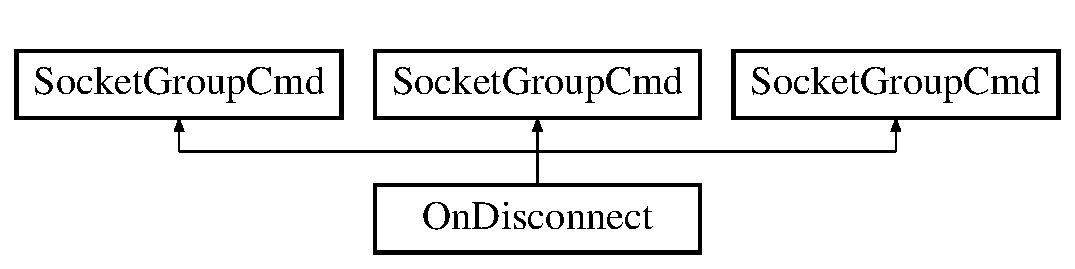
\includegraphics[height=2.000000cm]{classOnDisconnect}
\end{center}
\end{figure}


The documentation for this class was generated from the following files\+:\begin{DoxyCompactItemize}
\item 
/home/jc/metal/src/net\+Link/examples/smart\+\_\+buffer/web\+Get.\+cc\item 
/home/jc/metal/src/net\+Link/examples/socket\+\_\+group/chat\+Client.\+cc\item 
/home/jc/metal/src/net\+Link/examples/socket\+\_\+group/chat\+Server.\+cc\end{DoxyCompactItemize}

\hypertarget{classOnRead}{}\section{On\+Read Class Reference}
\label{classOnRead}\index{On\+Read@{On\+Read}}
Inheritance diagram for On\+Read\+:\begin{figure}[H]
\begin{center}
\leavevmode
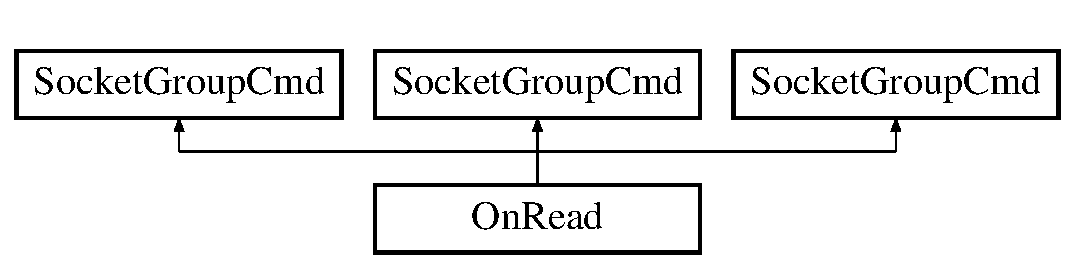
\includegraphics[height=2.000000cm]{classOnRead}
\end{center}
\end{figure}


The documentation for this class was generated from the following files\+:\begin{DoxyCompactItemize}
\item 
/home/jc/metal/github/src/3rdparties/net\+Link/examples/smart\+\_\+buffer/\hyperlink{webGet_8cc}{web\+Get.\+cc}\item 
/home/jc/metal/github/src/3rdparties/net\+Link/examples/socket\+\_\+group/\hyperlink{chatClient_8cc}{chat\+Client.\+cc}\item 
/home/jc/metal/github/src/3rdparties/net\+Link/examples/socket\+\_\+group/\hyperlink{chatServer_8cc}{chat\+Server.\+cc}\end{DoxyCompactItemize}

\hypertarget{classMetal_1_1OrderCancelRequest}{}\section{Metal\+:\+:Order\+Cancel\+Request Class Reference}
\label{classMetal_1_1OrderCancelRequest}\index{Metal\+::\+Order\+Cancel\+Request@{Metal\+::\+Order\+Cancel\+Request}}


{\ttfamily \#include $<$metal.\+h$>$}

Inheritance diagram for Metal\+:\+:Order\+Cancel\+Request\+:\begin{figure}[H]
\begin{center}
\leavevmode
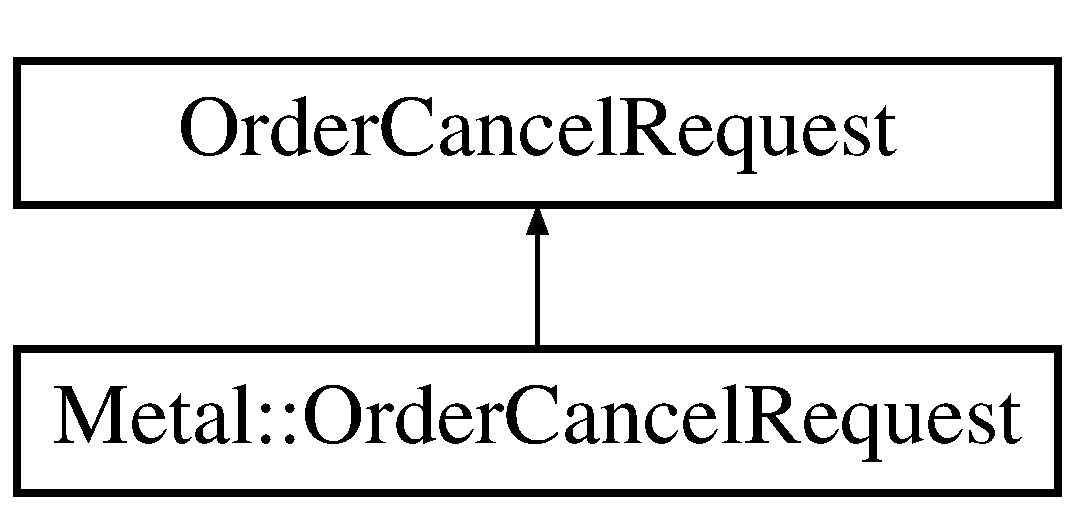
\includegraphics[height=2.000000cm]{classMetal_1_1OrderCancelRequest}
\end{center}
\end{figure}


The documentation for this class was generated from the following file\+:\begin{DoxyCompactItemize}
\item 
/home/jc/metal/github/include/metal/\hyperlink{metal_8h}{metal.\+h}\end{DoxyCompactItemize}

\hypertarget{classMetal_1_1LSE_1_1OrderCancelRequest}{}\section{Metal\+:\+:L\+S\+E\+:\+:Order\+Cancel\+Request Class Reference}
\label{classMetal_1_1LSE_1_1OrderCancelRequest}\index{Metal\+::\+L\+S\+E\+::\+Order\+Cancel\+Request@{Metal\+::\+L\+S\+E\+::\+Order\+Cancel\+Request}}


{\ttfamily \#include $<$Order\+Cancel\+Request.\+h$>$}

Inheritance diagram for Metal\+:\+:L\+S\+E\+:\+:Order\+Cancel\+Request\+:\begin{figure}[H]
\begin{center}
\leavevmode
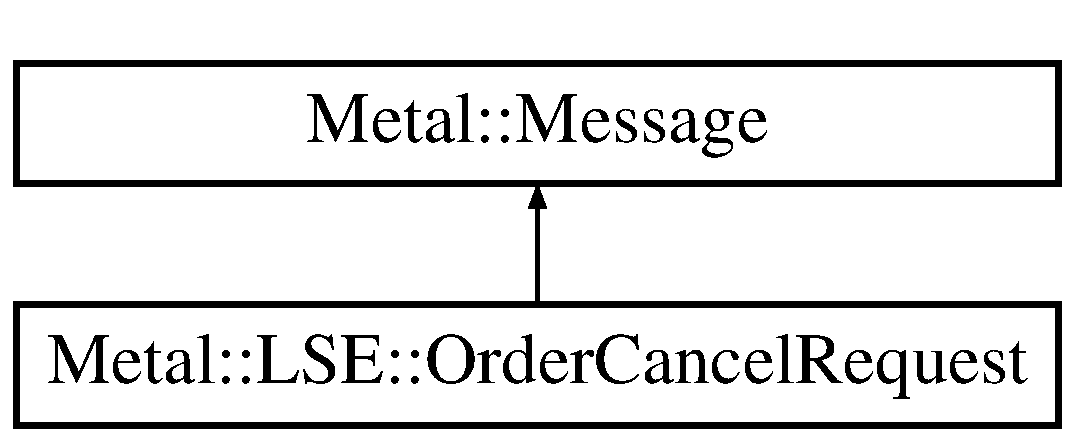
\includegraphics[height=2.000000cm]{classMetal_1_1LSE_1_1OrderCancelRequest}
\end{center}
\end{figure}
\subsection*{Public Member Functions}
\begin{DoxyCompactItemize}
\item 
\hyperlink{classMetal_1_1LSE_1_1OrderCancelRequest_a7334bf6b9c759c5d9c493fba0507111d}{Order\+Cancel\+Request} ()
\item 
virtual \hyperlink{classMetal_1_1LSE_1_1OrderCancelRequest_ada763ff79958a669d9255d8eb2028b60}{$\sim$\+Order\+Cancel\+Request} ()
\end{DoxyCompactItemize}
\subsection*{Public Attributes}
\begin{DoxyCompactItemize}
\item 
\hyperlink{namespaceMetal_1_1LSE_a7f5f027430e2d08dcf1a5ccba4ea7bc6}{Client\+Order\+I\+D} \hyperlink{classMetal_1_1LSE_1_1OrderCancelRequest_a17cf42a99f70826442cd78668a20e460}{client\+Order\+I\+D}
\item 
\hyperlink{namespaceMetal_1_1LSE_af5236b7a999484d8cd5b579b7d7c133b}{Side} \hyperlink{classMetal_1_1LSE_1_1OrderCancelRequest_a8147911f2234bdb988adfb6f43b7aaca}{side}
\item 
\hyperlink{namespaceMetal_1_1LSE_a30b8c9f132779cac1a35919835725059}{Order\+I\+D} \hyperlink{classMetal_1_1LSE_1_1OrderCancelRequest_ad35bf5f0e86e582724e8e6868028b976}{order\+Id}
\item 
\hyperlink{namespaceMetal_1_1LSE_a28d9de72a77b3eab8551831696a678c1}{Original\+Client\+Order\+I\+D} \hyperlink{classMetal_1_1LSE_1_1OrderCancelRequest_a96b6730c82337371d5de0354566a616c}{original\+Client\+Order\+Id}
\item 
\hyperlink{namespaceMetal_1_1LSE_a5280aa41aaa4433df351e733a23ecd14}{Instrument\+I\+D} \hyperlink{classMetal_1_1LSE_1_1OrderCancelRequest_a25a35022d18a4c0826199bbb6950ad16}{instrument\+I\+D}
\end{DoxyCompactItemize}
\subsection*{Additional Inherited Members}


\subsection{Constructor \& Destructor Documentation}
\hypertarget{classMetal_1_1LSE_1_1OrderCancelRequest_a7334bf6b9c759c5d9c493fba0507111d}{}\index{Metal\+::\+L\+S\+E\+::\+Order\+Cancel\+Request@{Metal\+::\+L\+S\+E\+::\+Order\+Cancel\+Request}!Order\+Cancel\+Request@{Order\+Cancel\+Request}}
\index{Order\+Cancel\+Request@{Order\+Cancel\+Request}!Metal\+::\+L\+S\+E\+::\+Order\+Cancel\+Request@{Metal\+::\+L\+S\+E\+::\+Order\+Cancel\+Request}}
\subsubsection[{Order\+Cancel\+Request}]{\setlength{\rightskip}{0pt plus 5cm}Metal\+::\+L\+S\+E\+::\+Order\+Cancel\+Request\+::\+Order\+Cancel\+Request (
\begin{DoxyParamCaption}
{}
\end{DoxyParamCaption}
)}\label{classMetal_1_1LSE_1_1OrderCancelRequest_a7334bf6b9c759c5d9c493fba0507111d}
\hypertarget{classMetal_1_1LSE_1_1OrderCancelRequest_ada763ff79958a669d9255d8eb2028b60}{}\index{Metal\+::\+L\+S\+E\+::\+Order\+Cancel\+Request@{Metal\+::\+L\+S\+E\+::\+Order\+Cancel\+Request}!````~Order\+Cancel\+Request@{$\sim$\+Order\+Cancel\+Request}}
\index{````~Order\+Cancel\+Request@{$\sim$\+Order\+Cancel\+Request}!Metal\+::\+L\+S\+E\+::\+Order\+Cancel\+Request@{Metal\+::\+L\+S\+E\+::\+Order\+Cancel\+Request}}
\subsubsection[{$\sim$\+Order\+Cancel\+Request}]{\setlength{\rightskip}{0pt plus 5cm}Metal\+::\+L\+S\+E\+::\+Order\+Cancel\+Request\+::$\sim$\+Order\+Cancel\+Request (
\begin{DoxyParamCaption}
{}
\end{DoxyParamCaption}
)\hspace{0.3cm}{\ttfamily [virtual]}}\label{classMetal_1_1LSE_1_1OrderCancelRequest_ada763ff79958a669d9255d8eb2028b60}


\subsection{Member Data Documentation}
\hypertarget{classMetal_1_1LSE_1_1OrderCancelRequest_a17cf42a99f70826442cd78668a20e460}{}\index{Metal\+::\+L\+S\+E\+::\+Order\+Cancel\+Request@{Metal\+::\+L\+S\+E\+::\+Order\+Cancel\+Request}!client\+Order\+I\+D@{client\+Order\+I\+D}}
\index{client\+Order\+I\+D@{client\+Order\+I\+D}!Metal\+::\+L\+S\+E\+::\+Order\+Cancel\+Request@{Metal\+::\+L\+S\+E\+::\+Order\+Cancel\+Request}}
\subsubsection[{client\+Order\+I\+D}]{\setlength{\rightskip}{0pt plus 5cm}{\bf Client\+Order\+I\+D} Metal\+::\+L\+S\+E\+::\+Order\+Cancel\+Request\+::client\+Order\+I\+D}\label{classMetal_1_1LSE_1_1OrderCancelRequest_a17cf42a99f70826442cd78668a20e460}
\hypertarget{classMetal_1_1LSE_1_1OrderCancelRequest_a25a35022d18a4c0826199bbb6950ad16}{}\index{Metal\+::\+L\+S\+E\+::\+Order\+Cancel\+Request@{Metal\+::\+L\+S\+E\+::\+Order\+Cancel\+Request}!instrument\+I\+D@{instrument\+I\+D}}
\index{instrument\+I\+D@{instrument\+I\+D}!Metal\+::\+L\+S\+E\+::\+Order\+Cancel\+Request@{Metal\+::\+L\+S\+E\+::\+Order\+Cancel\+Request}}
\subsubsection[{instrument\+I\+D}]{\setlength{\rightskip}{0pt plus 5cm}{\bf Instrument\+I\+D} Metal\+::\+L\+S\+E\+::\+Order\+Cancel\+Request\+::instrument\+I\+D}\label{classMetal_1_1LSE_1_1OrderCancelRequest_a25a35022d18a4c0826199bbb6950ad16}
\hypertarget{classMetal_1_1LSE_1_1OrderCancelRequest_ad35bf5f0e86e582724e8e6868028b976}{}\index{Metal\+::\+L\+S\+E\+::\+Order\+Cancel\+Request@{Metal\+::\+L\+S\+E\+::\+Order\+Cancel\+Request}!order\+Id@{order\+Id}}
\index{order\+Id@{order\+Id}!Metal\+::\+L\+S\+E\+::\+Order\+Cancel\+Request@{Metal\+::\+L\+S\+E\+::\+Order\+Cancel\+Request}}
\subsubsection[{order\+Id}]{\setlength{\rightskip}{0pt plus 5cm}{\bf Order\+I\+D} Metal\+::\+L\+S\+E\+::\+Order\+Cancel\+Request\+::order\+Id}\label{classMetal_1_1LSE_1_1OrderCancelRequest_ad35bf5f0e86e582724e8e6868028b976}
\hypertarget{classMetal_1_1LSE_1_1OrderCancelRequest_a96b6730c82337371d5de0354566a616c}{}\index{Metal\+::\+L\+S\+E\+::\+Order\+Cancel\+Request@{Metal\+::\+L\+S\+E\+::\+Order\+Cancel\+Request}!original\+Client\+Order\+Id@{original\+Client\+Order\+Id}}
\index{original\+Client\+Order\+Id@{original\+Client\+Order\+Id}!Metal\+::\+L\+S\+E\+::\+Order\+Cancel\+Request@{Metal\+::\+L\+S\+E\+::\+Order\+Cancel\+Request}}
\subsubsection[{original\+Client\+Order\+Id}]{\setlength{\rightskip}{0pt plus 5cm}{\bf Original\+Client\+Order\+I\+D} Metal\+::\+L\+S\+E\+::\+Order\+Cancel\+Request\+::original\+Client\+Order\+Id}\label{classMetal_1_1LSE_1_1OrderCancelRequest_a96b6730c82337371d5de0354566a616c}
\hypertarget{classMetal_1_1LSE_1_1OrderCancelRequest_a8147911f2234bdb988adfb6f43b7aaca}{}\index{Metal\+::\+L\+S\+E\+::\+Order\+Cancel\+Request@{Metal\+::\+L\+S\+E\+::\+Order\+Cancel\+Request}!side@{side}}
\index{side@{side}!Metal\+::\+L\+S\+E\+::\+Order\+Cancel\+Request@{Metal\+::\+L\+S\+E\+::\+Order\+Cancel\+Request}}
\subsubsection[{side}]{\setlength{\rightskip}{0pt plus 5cm}{\bf Side} Metal\+::\+L\+S\+E\+::\+Order\+Cancel\+Request\+::side}\label{classMetal_1_1LSE_1_1OrderCancelRequest_a8147911f2234bdb988adfb6f43b7aaca}


The documentation for this class was generated from the following files\+:\begin{DoxyCompactItemize}
\item 
/home/jc/metal/github/src/adapters/\+L\+S\+E\+Trading\+Adapter/\hyperlink{OrderCancelRequest_8h}{Order\+Cancel\+Request.\+h}\item 
/home/jc/metal/github/src/adapters/\+L\+S\+E\+Trading\+Adapter/\hyperlink{OrderCancelRequest_8cpp}{Order\+Cancel\+Request.\+cpp}\end{DoxyCompactItemize}

\hypertarget{classMetal_1_1QuickFIX_1_1QuickFIXAdapter}{}\section{Metal\+:\+:Quick\+F\+I\+X\+:\+:Quick\+F\+I\+X\+Adapter Class Reference}
\label{classMetal_1_1QuickFIX_1_1QuickFIXAdapter}\index{Metal\+::\+Quick\+F\+I\+X\+::\+Quick\+F\+I\+X\+Adapter@{Metal\+::\+Quick\+F\+I\+X\+::\+Quick\+F\+I\+X\+Adapter}}


{\ttfamily \#include $<$Quick\+F\+I\+X\+Adapter.\+h$>$}

Inheritance diagram for Metal\+:\+:Quick\+F\+I\+X\+:\+:Quick\+F\+I\+X\+Adapter\+:\begin{figure}[H]
\begin{center}
\leavevmode
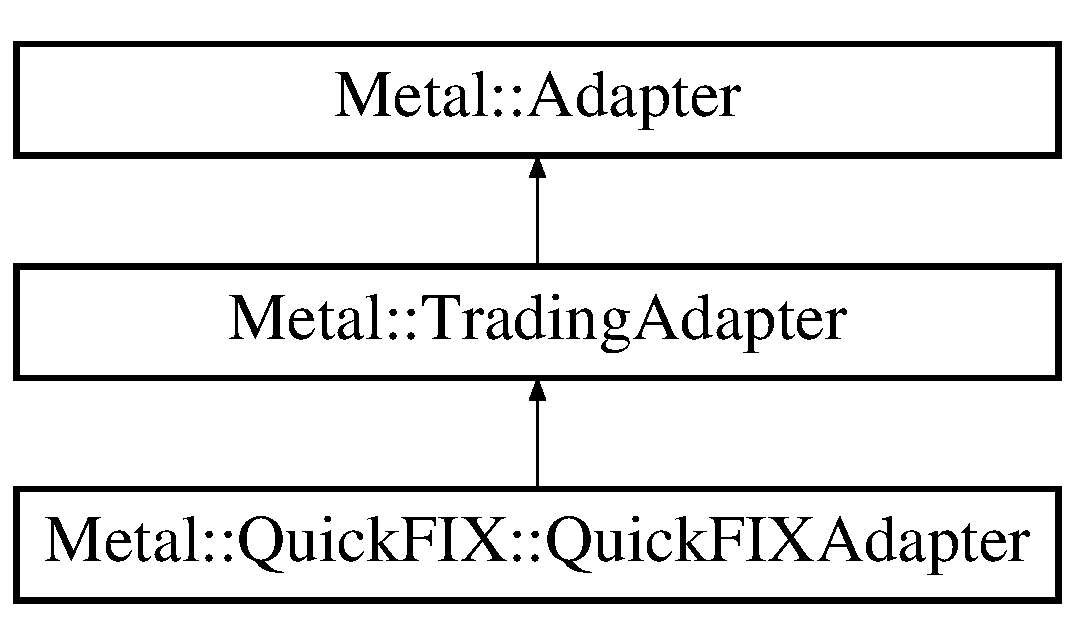
\includegraphics[height=3.000000cm]{classMetal_1_1QuickFIX_1_1QuickFIXAdapter}
\end{center}
\end{figure}
\subsection*{Public Member Functions}
\begin{DoxyCompactItemize}
\item 
\hyperlink{classMetal_1_1QuickFIX_1_1QuickFIXAdapter_ac437c5ed10c4b0ed06a49b31d194be70}{Quick\+F\+I\+X\+Adapter} ()
\item 
void \hyperlink{classMetal_1_1QuickFIX_1_1QuickFIXAdapter_ae53ab5057d4e2003a486ddc5761935a1}{send\+New\+Order} (const \hyperlink{classMetal_1_1NewOrderSingle}{New\+Order\+Single} \&nos)
\item 
virtual void \hyperlink{classMetal_1_1QuickFIX_1_1QuickFIXAdapter_acf1ae68d29b8a22c7252891665d218a8}{on\+Message} (const \hyperlink{namespaceMetal_af4294c176f6aecf9f75e9b106b117aa1}{Execution\+Report} \&er)
\item 
void \hyperlink{classMetal_1_1QuickFIX_1_1QuickFIXAdapter_a20f5db6305b3f479e12553f021765d60}{start} ()
\item 
void \hyperlink{classMetal_1_1QuickFIX_1_1QuickFIXAdapter_af0e438d5d64fa8a0aa3024b5a995f885}{stop} ()
\item 
virtual void \hyperlink{classMetal_1_1QuickFIX_1_1QuickFIXAdapter_ade65590a3da99272d88059e8f031b4d4}{encode\+Logon} (\hyperlink{classMetal_1_1Message}{Message} \&msg)
\item 
virtual void \hyperlink{classMetal_1_1QuickFIX_1_1QuickFIXAdapter_afa4aac6757cb58c2723eda4043156a4a}{encode\+Heart\+Beat} (\hyperlink{classMetal_1_1Message}{Message} \&msg)
\item 
virtual \hyperlink{classMetal_1_1QuickFIX_1_1QuickFIXAdapter_a3023c5d511ae87ee7a1cf73897fd09aa}{$\sim$\+Quick\+F\+I\+X\+Adapter} ()
\end{DoxyCompactItemize}
\subsection*{Static Public Attributes}
\begin{DoxyCompactItemize}
\item 
static const std\+::string \hyperlink{classMetal_1_1QuickFIX_1_1QuickFIXAdapter_aad5f72f920f26469fa0192dcbdb3a59a}{N\+A\+M\+E} = \char`\"{}Quick\+F\+I\+X\char`\"{}
\item 
static const std\+::string \hyperlink{classMetal_1_1QuickFIX_1_1QuickFIXAdapter_aa8a9ed777bdbc2c9a138fa35741da77a}{U\+U\+I\+D} = \char`\"{}e32cd5d0-\/4564-\/11e4-\/916c-\/0800200c9a66\char`\"{}
\end{DoxyCompactItemize}
\subsection*{Protected Member Functions}
\begin{DoxyCompactItemize}
\item 
int \hyperlink{classMetal_1_1QuickFIX_1_1QuickFIXAdapter_a0598785e8408706cde97d532090d3fcb}{process\+Data} (const char $\ast$data, int length)
\item 
void \hyperlink{classMetal_1_1QuickFIX_1_1QuickFIXAdapter_a6bb8af5a8dd9c4ad157bce0e8ef35ef1}{send\+Heart\+Beat} ()
\item 
void \hyperlink{classMetal_1_1QuickFIX_1_1QuickFIXAdapter_a3f9dba36bbaa3d8db8af62ac07a9fff5}{send\+Logon} ()
\end{DoxyCompactItemize}
\subsection*{Additional Inherited Members}


\subsection{Constructor \& Destructor Documentation}
\hypertarget{classMetal_1_1QuickFIX_1_1QuickFIXAdapter_ac437c5ed10c4b0ed06a49b31d194be70}{}\index{Metal\+::\+Quick\+F\+I\+X\+::\+Quick\+F\+I\+X\+Adapter@{Metal\+::\+Quick\+F\+I\+X\+::\+Quick\+F\+I\+X\+Adapter}!Quick\+F\+I\+X\+Adapter@{Quick\+F\+I\+X\+Adapter}}
\index{Quick\+F\+I\+X\+Adapter@{Quick\+F\+I\+X\+Adapter}!Metal\+::\+Quick\+F\+I\+X\+::\+Quick\+F\+I\+X\+Adapter@{Metal\+::\+Quick\+F\+I\+X\+::\+Quick\+F\+I\+X\+Adapter}}
\subsubsection[{Quick\+F\+I\+X\+Adapter}]{\setlength{\rightskip}{0pt plus 5cm}Metal\+::\+Quick\+F\+I\+X\+::\+Quick\+F\+I\+X\+Adapter\+::\+Quick\+F\+I\+X\+Adapter (
\begin{DoxyParamCaption}
{}
\end{DoxyParamCaption}
)}\label{classMetal_1_1QuickFIX_1_1QuickFIXAdapter_ac437c5ed10c4b0ed06a49b31d194be70}
Default Constructor \hypertarget{classMetal_1_1QuickFIX_1_1QuickFIXAdapter_a3023c5d511ae87ee7a1cf73897fd09aa}{}\index{Metal\+::\+Quick\+F\+I\+X\+::\+Quick\+F\+I\+X\+Adapter@{Metal\+::\+Quick\+F\+I\+X\+::\+Quick\+F\+I\+X\+Adapter}!````~Quick\+F\+I\+X\+Adapter@{$\sim$\+Quick\+F\+I\+X\+Adapter}}
\index{````~Quick\+F\+I\+X\+Adapter@{$\sim$\+Quick\+F\+I\+X\+Adapter}!Metal\+::\+Quick\+F\+I\+X\+::\+Quick\+F\+I\+X\+Adapter@{Metal\+::\+Quick\+F\+I\+X\+::\+Quick\+F\+I\+X\+Adapter}}
\subsubsection[{$\sim$\+Quick\+F\+I\+X\+Adapter}]{\setlength{\rightskip}{0pt plus 5cm}virtual Metal\+::\+Quick\+F\+I\+X\+::\+Quick\+F\+I\+X\+Adapter\+::$\sim$\+Quick\+F\+I\+X\+Adapter (
\begin{DoxyParamCaption}
{}
\end{DoxyParamCaption}
)\hspace{0.3cm}{\ttfamily [inline]}, {\ttfamily [virtual]}}\label{classMetal_1_1QuickFIX_1_1QuickFIXAdapter_a3023c5d511ae87ee7a1cf73897fd09aa}


\subsection{Member Function Documentation}
\hypertarget{classMetal_1_1QuickFIX_1_1QuickFIXAdapter_afa4aac6757cb58c2723eda4043156a4a}{}\index{Metal\+::\+Quick\+F\+I\+X\+::\+Quick\+F\+I\+X\+Adapter@{Metal\+::\+Quick\+F\+I\+X\+::\+Quick\+F\+I\+X\+Adapter}!encode\+Heart\+Beat@{encode\+Heart\+Beat}}
\index{encode\+Heart\+Beat@{encode\+Heart\+Beat}!Metal\+::\+Quick\+F\+I\+X\+::\+Quick\+F\+I\+X\+Adapter@{Metal\+::\+Quick\+F\+I\+X\+::\+Quick\+F\+I\+X\+Adapter}}
\subsubsection[{encode\+Heart\+Beat}]{\setlength{\rightskip}{0pt plus 5cm}virtual void Metal\+::\+Quick\+F\+I\+X\+::\+Quick\+F\+I\+X\+Adapter\+::encode\+Heart\+Beat (
\begin{DoxyParamCaption}
\item[{{\bf Message} \&}]{msg}
\end{DoxyParamCaption}
)\hspace{0.3cm}{\ttfamily [inline]}, {\ttfamily [virtual]}}\label{classMetal_1_1QuickFIX_1_1QuickFIXAdapter_afa4aac6757cb58c2723eda4043156a4a}
\hypertarget{classMetal_1_1QuickFIX_1_1QuickFIXAdapter_ade65590a3da99272d88059e8f031b4d4}{}\index{Metal\+::\+Quick\+F\+I\+X\+::\+Quick\+F\+I\+X\+Adapter@{Metal\+::\+Quick\+F\+I\+X\+::\+Quick\+F\+I\+X\+Adapter}!encode\+Logon@{encode\+Logon}}
\index{encode\+Logon@{encode\+Logon}!Metal\+::\+Quick\+F\+I\+X\+::\+Quick\+F\+I\+X\+Adapter@{Metal\+::\+Quick\+F\+I\+X\+::\+Quick\+F\+I\+X\+Adapter}}
\subsubsection[{encode\+Logon}]{\setlength{\rightskip}{0pt plus 5cm}virtual void Metal\+::\+Quick\+F\+I\+X\+::\+Quick\+F\+I\+X\+Adapter\+::encode\+Logon (
\begin{DoxyParamCaption}
\item[{{\bf Message} \&}]{msg}
\end{DoxyParamCaption}
)\hspace{0.3cm}{\ttfamily [inline]}, {\ttfamily [virtual]}}\label{classMetal_1_1QuickFIX_1_1QuickFIXAdapter_ade65590a3da99272d88059e8f031b4d4}
We don't need to provide \hyperlink{classMetal_1_1Logon}{Logon} Encoding because \hyperlink{namespaceMetal_1_1QuickFIX}{Quick\+F\+I\+X} provides its own session management \hypertarget{classMetal_1_1QuickFIX_1_1QuickFIXAdapter_acf1ae68d29b8a22c7252891665d218a8}{}\index{Metal\+::\+Quick\+F\+I\+X\+::\+Quick\+F\+I\+X\+Adapter@{Metal\+::\+Quick\+F\+I\+X\+::\+Quick\+F\+I\+X\+Adapter}!on\+Message@{on\+Message}}
\index{on\+Message@{on\+Message}!Metal\+::\+Quick\+F\+I\+X\+::\+Quick\+F\+I\+X\+Adapter@{Metal\+::\+Quick\+F\+I\+X\+::\+Quick\+F\+I\+X\+Adapter}}
\subsubsection[{on\+Message}]{\setlength{\rightskip}{0pt plus 5cm}void Metal\+::\+Quick\+F\+I\+X\+::\+Quick\+F\+I\+X\+Adapter\+::on\+Message (
\begin{DoxyParamCaption}
\item[{const {\bf Execution\+Report} \&}]{er}
\end{DoxyParamCaption}
)\hspace{0.3cm}{\ttfamily [virtual]}}\label{classMetal_1_1QuickFIX_1_1QuickFIXAdapter_acf1ae68d29b8a22c7252891665d218a8}
This method will invoked upon receiving a normalized execution report~\newline
 Subclasses should override this method to capture execution reports in generic format~\newline
 
\begin{DoxyParams}{Parameters}
{\em Execution\+Report} & incomming execution report \\
\hline
\end{DoxyParams}


Reimplemented from \hyperlink{classMetal_1_1TradingAdapter_a44332505b213c0428d901ef6a530efff}{Metal\+::\+Trading\+Adapter}.

\hypertarget{classMetal_1_1QuickFIX_1_1QuickFIXAdapter_a0598785e8408706cde97d532090d3fcb}{}\index{Metal\+::\+Quick\+F\+I\+X\+::\+Quick\+F\+I\+X\+Adapter@{Metal\+::\+Quick\+F\+I\+X\+::\+Quick\+F\+I\+X\+Adapter}!process\+Data@{process\+Data}}
\index{process\+Data@{process\+Data}!Metal\+::\+Quick\+F\+I\+X\+::\+Quick\+F\+I\+X\+Adapter@{Metal\+::\+Quick\+F\+I\+X\+::\+Quick\+F\+I\+X\+Adapter}}
\subsubsection[{process\+Data}]{\setlength{\rightskip}{0pt plus 5cm}int Metal\+::\+Quick\+F\+I\+X\+::\+Quick\+F\+I\+X\+Adapter\+::process\+Data (
\begin{DoxyParamCaption}
\item[{const char $\ast$}]{data, }
\item[{int}]{length}
\end{DoxyParamCaption}
)\hspace{0.3cm}{\ttfamily [inline]}, {\ttfamily [protected]}, {\ttfamily [virtual]}}\label{classMetal_1_1QuickFIX_1_1QuickFIXAdapter_a0598785e8408706cde97d532090d3fcb}
We don't implement a real data processor because we are leveraging \hyperlink{namespaceMetal_1_1QuickFIX}{Quick\+F\+I\+X} parsing ability 

Implements \hyperlink{classMetal_1_1Adapter_a195072772568dc0fd7a859ed2c99d5c7}{Metal\+::\+Adapter}.

\hypertarget{classMetal_1_1QuickFIX_1_1QuickFIXAdapter_a6bb8af5a8dd9c4ad157bce0e8ef35ef1}{}\index{Metal\+::\+Quick\+F\+I\+X\+::\+Quick\+F\+I\+X\+Adapter@{Metal\+::\+Quick\+F\+I\+X\+::\+Quick\+F\+I\+X\+Adapter}!send\+Heart\+Beat@{send\+Heart\+Beat}}
\index{send\+Heart\+Beat@{send\+Heart\+Beat}!Metal\+::\+Quick\+F\+I\+X\+::\+Quick\+F\+I\+X\+Adapter@{Metal\+::\+Quick\+F\+I\+X\+::\+Quick\+F\+I\+X\+Adapter}}
\subsubsection[{send\+Heart\+Beat}]{\setlength{\rightskip}{0pt plus 5cm}void Metal\+::\+Quick\+F\+I\+X\+::\+Quick\+F\+I\+X\+Adapter\+::send\+Heart\+Beat (
\begin{DoxyParamCaption}
{}
\end{DoxyParamCaption}
)\hspace{0.3cm}{\ttfamily [inline]}, {\ttfamily [protected]}, {\ttfamily [virtual]}}\label{classMetal_1_1QuickFIX_1_1QuickFIXAdapter_a6bb8af5a8dd9c4ad157bce0e8ef35ef1}
Formats and sends a Heart Beat message 

Implements \hyperlink{classMetal_1_1TradingAdapter_a39caec739aaad9593ba1b93b8e130385}{Metal\+::\+Trading\+Adapter}.

\hypertarget{classMetal_1_1QuickFIX_1_1QuickFIXAdapter_a3f9dba36bbaa3d8db8af62ac07a9fff5}{}\index{Metal\+::\+Quick\+F\+I\+X\+::\+Quick\+F\+I\+X\+Adapter@{Metal\+::\+Quick\+F\+I\+X\+::\+Quick\+F\+I\+X\+Adapter}!send\+Logon@{send\+Logon}}
\index{send\+Logon@{send\+Logon}!Metal\+::\+Quick\+F\+I\+X\+::\+Quick\+F\+I\+X\+Adapter@{Metal\+::\+Quick\+F\+I\+X\+::\+Quick\+F\+I\+X\+Adapter}}
\subsubsection[{send\+Logon}]{\setlength{\rightskip}{0pt plus 5cm}void Metal\+::\+Quick\+F\+I\+X\+::\+Quick\+F\+I\+X\+Adapter\+::send\+Logon (
\begin{DoxyParamCaption}
{}
\end{DoxyParamCaption}
)\hspace{0.3cm}{\ttfamily [inline]}, {\ttfamily [protected]}, {\ttfamily [virtual]}}\label{classMetal_1_1QuickFIX_1_1QuickFIXAdapter_a3f9dba36bbaa3d8db8af62ac07a9fff5}
Sends a logon message to initiate the session 

Implements \hyperlink{classMetal_1_1TradingAdapter_a39562015df3e7202a5e8f932b8bde43e}{Metal\+::\+Trading\+Adapter}.

\hypertarget{classMetal_1_1QuickFIX_1_1QuickFIXAdapter_ae53ab5057d4e2003a486ddc5761935a1}{}\index{Metal\+::\+Quick\+F\+I\+X\+::\+Quick\+F\+I\+X\+Adapter@{Metal\+::\+Quick\+F\+I\+X\+::\+Quick\+F\+I\+X\+Adapter}!send\+New\+Order@{send\+New\+Order}}
\index{send\+New\+Order@{send\+New\+Order}!Metal\+::\+Quick\+F\+I\+X\+::\+Quick\+F\+I\+X\+Adapter@{Metal\+::\+Quick\+F\+I\+X\+::\+Quick\+F\+I\+X\+Adapter}}
\subsubsection[{send\+New\+Order}]{\setlength{\rightskip}{0pt plus 5cm}void Metal\+::\+Quick\+F\+I\+X\+::\+Quick\+F\+I\+X\+Adapter\+::send\+New\+Order (
\begin{DoxyParamCaption}
\item[{const {\bf New\+Order\+Single} \&}]{nos}
\end{DoxyParamCaption}
)\hspace{0.3cm}{\ttfamily [virtual]}}\label{classMetal_1_1QuickFIX_1_1QuickFIXAdapter_ae53ab5057d4e2003a486ddc5761935a1}
We override this method to leverage \hyperlink{namespaceMetal_1_1QuickFIX}{Quick\+F\+I\+X} sending capacity

Send normalized New Order 

Implements \hyperlink{classMetal_1_1TradingAdapter_abccc3fdb238887112e1a0820a70f0fce}{Metal\+::\+Trading\+Adapter}.

\hypertarget{classMetal_1_1QuickFIX_1_1QuickFIXAdapter_a20f5db6305b3f479e12553f021765d60}{}\index{Metal\+::\+Quick\+F\+I\+X\+::\+Quick\+F\+I\+X\+Adapter@{Metal\+::\+Quick\+F\+I\+X\+::\+Quick\+F\+I\+X\+Adapter}!start@{start}}
\index{start@{start}!Metal\+::\+Quick\+F\+I\+X\+::\+Quick\+F\+I\+X\+Adapter@{Metal\+::\+Quick\+F\+I\+X\+::\+Quick\+F\+I\+X\+Adapter}}
\subsubsection[{start}]{\setlength{\rightskip}{0pt plus 5cm}void Metal\+::\+Quick\+F\+I\+X\+::\+Quick\+F\+I\+X\+Adapter\+::start (
\begin{DoxyParamCaption}
{}
\end{DoxyParamCaption}
)\hspace{0.3cm}{\ttfamily [virtual]}}\label{classMetal_1_1QuickFIX_1_1QuickFIXAdapter_a20f5db6305b3f479e12553f021765d60}
We are overidding start to prevent \hyperlink{classMetal_1_1Adapter}{Adapter} processing of session life cycle 

Reimplemented from \hyperlink{classMetal_1_1Adapter_adeed43dfa9e2d18bd66dd2f806b1e182}{Metal\+::\+Adapter}.

\hypertarget{classMetal_1_1QuickFIX_1_1QuickFIXAdapter_af0e438d5d64fa8a0aa3024b5a995f885}{}\index{Metal\+::\+Quick\+F\+I\+X\+::\+Quick\+F\+I\+X\+Adapter@{Metal\+::\+Quick\+F\+I\+X\+::\+Quick\+F\+I\+X\+Adapter}!stop@{stop}}
\index{stop@{stop}!Metal\+::\+Quick\+F\+I\+X\+::\+Quick\+F\+I\+X\+Adapter@{Metal\+::\+Quick\+F\+I\+X\+::\+Quick\+F\+I\+X\+Adapter}}
\subsubsection[{stop}]{\setlength{\rightskip}{0pt plus 5cm}void Metal\+::\+Quick\+F\+I\+X\+::\+Quick\+F\+I\+X\+Adapter\+::stop (
\begin{DoxyParamCaption}
{}
\end{DoxyParamCaption}
)}\label{classMetal_1_1QuickFIX_1_1QuickFIXAdapter_af0e438d5d64fa8a0aa3024b5a995f885}


\subsection{Member Data Documentation}
\hypertarget{classMetal_1_1QuickFIX_1_1QuickFIXAdapter_aad5f72f920f26469fa0192dcbdb3a59a}{}\index{Metal\+::\+Quick\+F\+I\+X\+::\+Quick\+F\+I\+X\+Adapter@{Metal\+::\+Quick\+F\+I\+X\+::\+Quick\+F\+I\+X\+Adapter}!N\+A\+M\+E@{N\+A\+M\+E}}
\index{N\+A\+M\+E@{N\+A\+M\+E}!Metal\+::\+Quick\+F\+I\+X\+::\+Quick\+F\+I\+X\+Adapter@{Metal\+::\+Quick\+F\+I\+X\+::\+Quick\+F\+I\+X\+Adapter}}
\subsubsection[{N\+A\+M\+E}]{\setlength{\rightskip}{0pt plus 5cm}const std\+::string Metal\+::\+Quick\+F\+I\+X\+::\+Quick\+F\+I\+X\+Adapter\+::\+N\+A\+M\+E = \char`\"{}Quick\+F\+I\+X\char`\"{}\hspace{0.3cm}{\ttfamily [static]}}\label{classMetal_1_1QuickFIX_1_1QuickFIXAdapter_aad5f72f920f26469fa0192dcbdb3a59a}
\hypertarget{classMetal_1_1QuickFIX_1_1QuickFIXAdapter_aa8a9ed777bdbc2c9a138fa35741da77a}{}\index{Metal\+::\+Quick\+F\+I\+X\+::\+Quick\+F\+I\+X\+Adapter@{Metal\+::\+Quick\+F\+I\+X\+::\+Quick\+F\+I\+X\+Adapter}!U\+U\+I\+D@{U\+U\+I\+D}}
\index{U\+U\+I\+D@{U\+U\+I\+D}!Metal\+::\+Quick\+F\+I\+X\+::\+Quick\+F\+I\+X\+Adapter@{Metal\+::\+Quick\+F\+I\+X\+::\+Quick\+F\+I\+X\+Adapter}}
\subsubsection[{U\+U\+I\+D}]{\setlength{\rightskip}{0pt plus 5cm}const std\+::string Metal\+::\+Quick\+F\+I\+X\+::\+Quick\+F\+I\+X\+Adapter\+::\+U\+U\+I\+D = \char`\"{}e32cd5d0-\/4564-\/11e4-\/916c-\/0800200c9a66\char`\"{}\hspace{0.3cm}{\ttfamily [static]}}\label{classMetal_1_1QuickFIX_1_1QuickFIXAdapter_aa8a9ed777bdbc2c9a138fa35741da77a}


The documentation for this class was generated from the following files\+:\begin{DoxyCompactItemize}
\item 
/home/jc/metal/github/src/adapters/\+Quick\+F\+I\+X\+Adapter/\hyperlink{QuickFIXAdapter_8h}{Quick\+F\+I\+X\+Adapter.\+h}\item 
/home/jc/metal/github/src/adapters/\+Quick\+F\+I\+X\+Adapter/\hyperlink{QuickFIXAdapter_8cpp}{Quick\+F\+I\+X\+Adapter.\+cpp}\end{DoxyCompactItemize}

\hypertarget{classMetal_1_1QuickFIXMessageMapper}{}\section{Metal\+:\+:Quick\+F\+I\+X\+Message\+Mapper Class Reference}
\label{classMetal_1_1QuickFIXMessageMapper}\index{Metal\+::\+Quick\+F\+I\+X\+Message\+Mapper@{Metal\+::\+Quick\+F\+I\+X\+Message\+Mapper}}
Inheritance diagram for Metal\+:\+:Quick\+F\+I\+X\+Message\+Mapper\+:\begin{figure}[H]
\begin{center}
\leavevmode
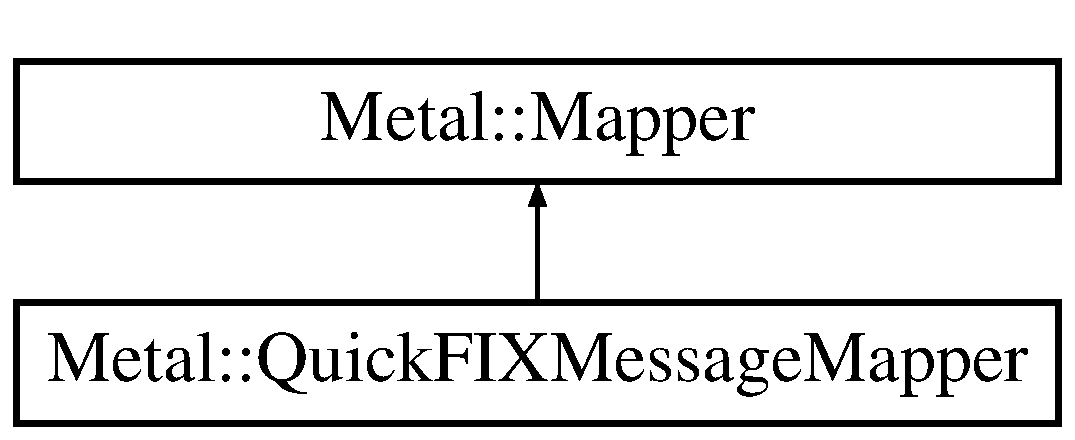
\includegraphics[height=2.000000cm]{classMetal_1_1QuickFIXMessageMapper}
\end{center}
\end{figure}
\subsection*{Static Public Member Functions}
\begin{DoxyCompactItemize}
\item 
static void \hyperlink{classMetal_1_1QuickFIXMessageMapper_ad42b0f6ed92b6e777e3716de55b20f21}{map} (const F\+I\+X44\+::\+New\+Order\+Single \&, \hyperlink{classMetal_1_1NewOrderSingle}{New\+Order\+Single} \&)
\item 
static void \hyperlink{classMetal_1_1QuickFIXMessageMapper_a98184463c76af4e0a21e8dfbd4b61af4}{map} (const F\+I\+X44\+::\+Execution\+Report \&, Execution\+Report \&)
\item 
static void \hyperlink{classMetal_1_1QuickFIXMessageMapper_ad5c9c32bc745db35e7d2a472cb204514}{map} (const \hyperlink{classMetal_1_1NewOrderSingle}{New\+Order\+Single} \&, F\+I\+X\+::\+Message \&)
\item 
static void \hyperlink{classMetal_1_1QuickFIXMessageMapper_ab7692db7b3f7b616acd7c6e9fc024d2c}{map} (const \hyperlink{classMetal_1_1OrderCancelRequest}{Order\+Cancel\+Request} \&, F\+I\+X\+::\+Message \&)
\end{DoxyCompactItemize}


\subsection{Member Function Documentation}
\hypertarget{classMetal_1_1QuickFIXMessageMapper_ad42b0f6ed92b6e777e3716de55b20f21}{}\index{Metal\+::\+Quick\+F\+I\+X\+Message\+Mapper@{Metal\+::\+Quick\+F\+I\+X\+Message\+Mapper}!map@{map}}
\index{map@{map}!Metal\+::\+Quick\+F\+I\+X\+Message\+Mapper@{Metal\+::\+Quick\+F\+I\+X\+Message\+Mapper}}
\subsubsection[{map}]{\setlength{\rightskip}{0pt plus 5cm}void Metal\+::\+Quick\+F\+I\+X\+Message\+Mapper\+::map (
\begin{DoxyParamCaption}
\item[{const F\+I\+X44\+::\+New\+Order\+Single \&}]{message, }
\item[{{\bf New\+Order\+Single} \&}]{nos}
\end{DoxyParamCaption}
)\hspace{0.3cm}{\ttfamily [static]}}\label{classMetal_1_1QuickFIXMessageMapper_ad42b0f6ed92b6e777e3716de55b20f21}
Translate F\+I\+X \hyperlink{classMetal_1_1NewOrderSingle}{New\+Order\+Single} into Metal representation \hypertarget{classMetal_1_1QuickFIXMessageMapper_a98184463c76af4e0a21e8dfbd4b61af4}{}\index{Metal\+::\+Quick\+F\+I\+X\+Message\+Mapper@{Metal\+::\+Quick\+F\+I\+X\+Message\+Mapper}!map@{map}}
\index{map@{map}!Metal\+::\+Quick\+F\+I\+X\+Message\+Mapper@{Metal\+::\+Quick\+F\+I\+X\+Message\+Mapper}}
\subsubsection[{map}]{\setlength{\rightskip}{0pt plus 5cm}void Metal\+::\+Quick\+F\+I\+X\+Message\+Mapper\+::map (
\begin{DoxyParamCaption}
\item[{const F\+I\+X44\+::\+Execution\+Report \&}]{message, }
\item[{Execution\+Report \&}]{er}
\end{DoxyParamCaption}
)\hspace{0.3cm}{\ttfamily [static]}}\label{classMetal_1_1QuickFIXMessageMapper_a98184463c76af4e0a21e8dfbd4b61af4}
Execution Report F\+I\+X -\/$>$ Me\+T\+A\+L \hypertarget{classMetal_1_1QuickFIXMessageMapper_ad5c9c32bc745db35e7d2a472cb204514}{}\index{Metal\+::\+Quick\+F\+I\+X\+Message\+Mapper@{Metal\+::\+Quick\+F\+I\+X\+Message\+Mapper}!map@{map}}
\index{map@{map}!Metal\+::\+Quick\+F\+I\+X\+Message\+Mapper@{Metal\+::\+Quick\+F\+I\+X\+Message\+Mapper}}
\subsubsection[{map}]{\setlength{\rightskip}{0pt plus 5cm}void Metal\+::\+Quick\+F\+I\+X\+Message\+Mapper\+::map (
\begin{DoxyParamCaption}
\item[{const {\bf New\+Order\+Single} \&}]{nos, }
\item[{F\+I\+X\+::\+Message \&}]{message}
\end{DoxyParamCaption}
)\hspace{0.3cm}{\ttfamily [static]}}\label{classMetal_1_1QuickFIXMessageMapper_ad5c9c32bc745db35e7d2a472cb204514}
Me\+T\+A\+L to F\+I\+X44 transformation for \hyperlink{classMetal_1_1NewOrderSingle}{New\+Order\+Single}

\hyperlink{classMetal_1_1NewOrderSingle}{New\+Order\+Single} Me\+T\+A\+L -\/$>$ F\+I\+X44 \hypertarget{classMetal_1_1QuickFIXMessageMapper_ab7692db7b3f7b616acd7c6e9fc024d2c}{}\index{Metal\+::\+Quick\+F\+I\+X\+Message\+Mapper@{Metal\+::\+Quick\+F\+I\+X\+Message\+Mapper}!map@{map}}
\index{map@{map}!Metal\+::\+Quick\+F\+I\+X\+Message\+Mapper@{Metal\+::\+Quick\+F\+I\+X\+Message\+Mapper}}
\subsubsection[{map}]{\setlength{\rightskip}{0pt plus 5cm}void Metal\+::\+Quick\+F\+I\+X\+Message\+Mapper\+::map (
\begin{DoxyParamCaption}
\item[{const {\bf Order\+Cancel\+Request} \&}]{ocr, }
\item[{F\+I\+X\+::\+Message \&}]{message}
\end{DoxyParamCaption}
)\hspace{0.3cm}{\ttfamily [static]}}\label{classMetal_1_1QuickFIXMessageMapper_ab7692db7b3f7b616acd7c6e9fc024d2c}
Me\+T\+A\+L to F\+I\+X44 transformation for \hyperlink{classMetal_1_1OrderCancelRequest}{Order\+Cancel\+Request} 

The documentation for this class was generated from the following files\+:\begin{DoxyCompactItemize}
\item 
/home/jc/metal/src/metal/adapters/\+Quick\+F\+I\+X\+Adapter/Quick\+F\+I\+X\+Message\+Mapper.\+h\item 
/home/jc/metal/src/metal/adapters/\+Quick\+F\+I\+X\+Adapter/Quick\+F\+I\+X\+Message\+Mapper.\+cpp\end{DoxyCompactItemize}

\hypertarget{classReleaseManager}{}\section{Release\+Manager$<$ T $>$ Class Template Reference}
\label{classReleaseManager}\index{Release\+Manager$<$ T $>$@{Release\+Manager$<$ T $>$}}


{\ttfamily \#include $<$netlink/release\+\_\+manager.\+h$>$}

\subsection*{Public Member Functions}
\begin{DoxyCompactItemize}
\item 
\hypertarget{classReleaseManager_a52cd29519b454a83dffdb282e601acfa}{}{\bfseries Release\+Manager} (void($\ast$release\+Function)(T $\ast$)=N\+U\+L\+L)\label{classReleaseManager_a52cd29519b454a83dffdb282e601acfa}

\item 
\hypertarget{classReleaseManager_a4cbea873df1e51c2d337e201623d8a67}{}void {\bfseries add} (T $\ast$$\ast$var)\label{classReleaseManager_a4cbea873df1e51c2d337e201623d8a67}

\item 
\hypertarget{classReleaseManager_af2dc4d35911de92c4b84f9be82e6e25b}{}void {\bfseries add} (T $\ast$address)\label{classReleaseManager_af2dc4d35911de92c4b84f9be82e6e25b}

\end{DoxyCompactItemize}
\subsection*{Protected Attributes}
\begin{DoxyCompactItemize}
\item 
\hypertarget{classReleaseManager_a377023e66c1ecd5cf0d16a80e1a9b0bb}{}vector$<$ T $\ast$$\ast$ $>$ {\bfseries \+\_\+release\+Queue}\label{classReleaseManager_a377023e66c1ecd5cf0d16a80e1a9b0bb}

\item 
\hypertarget{classReleaseManager_ac8a2b36b8540e109cb1ea89cea83c4e8}{}vector$<$ T $\ast$ $>$ {\bfseries \+\_\+release\+Address\+Queue}\label{classReleaseManager_ac8a2b36b8540e109cb1ea89cea83c4e8}

\item 
\hypertarget{classReleaseManager_a3a011107bd8d4ea8d7b955c59098d73c}{}void($\ast$ {\bfseries \+\_\+release\+Function} )(T $\ast$)\label{classReleaseManager_a3a011107bd8d4ea8d7b955c59098d73c}

\end{DoxyCompactItemize}


\subsection{Detailed Description}
\subsubsection*{template$<$typename T$>$class Release\+Manager$<$ T $>$}

Release Manager Class

Private. For internal use 

The documentation for this class was generated from the following files\+:\begin{DoxyCompactItemize}
\item 
/home/jc/metal/src/net\+Link/include/netlink/release\+\_\+manager.\+h\item 
/home/jc/metal/src/net\+Link/include/netlink/release\+\_\+manager.\+inline.\+h\end{DoxyCompactItemize}

\hypertarget{classMetal_1_1SendMessageException}{}\section{Metal\+:\+:Send\+Message\+Exception Class Reference}
\label{classMetal_1_1SendMessageException}\index{Metal\+::\+Send\+Message\+Exception@{Metal\+::\+Send\+Message\+Exception}}
Inheritance diagram for Metal\+:\+:Send\+Message\+Exception\+:\begin{figure}[H]
\begin{center}
\leavevmode
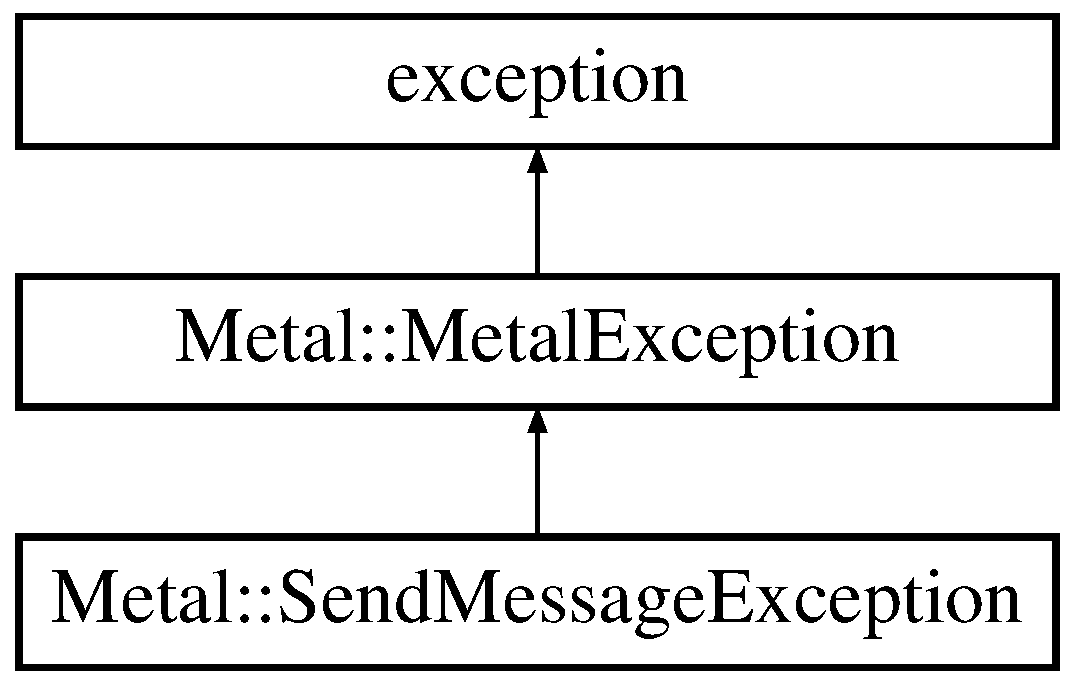
\includegraphics[height=3.000000cm]{classMetal_1_1SendMessageException}
\end{center}
\end{figure}
\subsection*{Public Member Functions}
\begin{DoxyCompactItemize}
\item 
\hypertarget{classMetal_1_1SendMessageException_a4aeb690808ab3639bbd837b7c57cc419}{}{\bfseries Send\+Message\+Exception} (const std\+::string \&message)\label{classMetal_1_1SendMessageException_a4aeb690808ab3639bbd837b7c57cc419}

\end{DoxyCompactItemize}


The documentation for this class was generated from the following file\+:\begin{DoxyCompactItemize}
\item 
/home/jc/metal/src/metal/Metal\+Exceptions.\+h\end{DoxyCompactItemize}

\hypertarget{classSmartBuffer}{}\section{Smart\+Buffer Class Reference}
\label{classSmartBuffer}\index{Smart\+Buffer@{Smart\+Buffer}}


{\ttfamily \#include $<$netlink/smart\+\_\+buffer.\+h$>$}

\subsection*{Public Member Functions}
\begin{DoxyCompactItemize}
\item 
\hyperlink{classSmartBuffer_ae7b059bbd714dcda7386b11c7e00ee0d}{Smart\+Buffer} (size\+\_\+t alloc\+Size=D\+E\+F\+A\+U\+L\+T\+\_\+\+S\+M\+A\+R\+T\+B\+U\+F\+F\+E\+R\+\_\+\+S\+I\+Z\+E, double realloc\+Ratio=D\+E\+F\+A\+U\+L\+T\+\_\+\+S\+M\+A\+R\+T\+B\+U\+F\+F\+E\+R\+\_\+\+R\+E\+A\+L\+L\+O\+C\+\_\+\+R\+A\+T\+I\+O)
\item 
\hyperlink{classSmartBuffer_a9058e1103bf628a075415390b02bffc2}{Smart\+Buffer} (\hyperlink{classSmartBuffer}{Smart\+Buffer} \&s)
\item 
\hyperlink{classSmartBuffer_a4ee71a48ec838b2b5ef43a32c5de8126}{$\sim$\+Smart\+Buffer} ()
\item 
const void $\ast$ \hyperlink{classSmartBuffer_afc1dc164bd7107b515b2d0642fdc5d43}{operator$\ast$} () const 
\item 
const char $\ast$ \hyperlink{classSmartBuffer_a8e17ba4a6f2f8dfdbe368469201fc4ef}{operator\mbox{[}$\,$\mbox{]}} (size\+\_\+t index) const 
\item 
const void $\ast$ \hyperlink{classSmartBuffer_a4a65be9a7a1e3c1914ffccf35a35f3f1}{buffer} () const 
\item 
size\+\_\+t \hyperlink{classSmartBuffer_aa2246cfac251b00cbaeb3763fa1aa11e}{size} () const 
\item 
void \hyperlink{classSmartBuffer_abb25b6f9ab458ee2eadde5f42c377f4e}{read} (\hyperlink{classSocket}{Socket} $\ast$socket)
\item 
void \hyperlink{classSmartBuffer_a6b1e284efe0d8c04bd964016a83340b3}{clear} ()
\item 
\hyperlink{classSmartBuffer}{Smart\+Buffer} \& \hyperlink{classSmartBuffer_aad00b9914962b562c6d59e2391b9deb3}{operator=} (\hyperlink{classSmartBuffer}{Smart\+Buffer} \&s)
\end{DoxyCompactItemize}


\subsection{Detailed Description}
Smart Buffer Class

Buffer class to retrieve data of unknown size easily from a \hyperlink{classSocket}{Socket} 

\subsection{Constructor \& Destructor Documentation}
\hypertarget{classSmartBuffer_ae7b059bbd714dcda7386b11c7e00ee0d}{}\index{Smart\+Buffer@{Smart\+Buffer}!Smart\+Buffer@{Smart\+Buffer}}
\index{Smart\+Buffer@{Smart\+Buffer}!Smart\+Buffer@{Smart\+Buffer}}
\subsubsection[{Smart\+Buffer}]{\setlength{\rightskip}{0pt plus 5cm}Smart\+Buffer\+::\+Smart\+Buffer (
\begin{DoxyParamCaption}
\item[{size\+\_\+t}]{alloc\+Size = {\ttfamily DEFAULT\+\_\+SMARTBUFFER\+\_\+SIZE}, }
\item[{double}]{realloc\+Ratio = {\ttfamily DEFAULT\+\_\+SMARTBUFFER\+\_\+REALLOC\+\_\+RATIO}}
\end{DoxyParamCaption}
)}\label{classSmartBuffer_ae7b059bbd714dcda7386b11c7e00ee0d}
\hyperlink{classSmartBuffer}{Smart\+Buffer} Constructor


\begin{DoxyParams}{Parameters}
{\em alloc\+Size} & Size in bytes of the initial reserved memory. \\
\hline
{\em realloc\+Ratio} & Growing ratio for memory reallocs. For example 1.\+5 means that each time the buffer is out of memory it reserves the previous size 1.\+5 times (150\%).\\
\hline
\end{DoxyParams}

\begin{DoxyExceptions}{Exceptions}
{\em \hyperlink{classException}{Exception}} & E\+R\+R\+O\+R\+\_\+\+A\+L\+L\+O\+C \\
\hline
\end{DoxyExceptions}
\hypertarget{classSmartBuffer_a9058e1103bf628a075415390b02bffc2}{}\index{Smart\+Buffer@{Smart\+Buffer}!Smart\+Buffer@{Smart\+Buffer}}
\index{Smart\+Buffer@{Smart\+Buffer}!Smart\+Buffer@{Smart\+Buffer}}
\subsubsection[{Smart\+Buffer}]{\setlength{\rightskip}{0pt plus 5cm}Smart\+Buffer\+::\+Smart\+Buffer (
\begin{DoxyParamCaption}
\item[{{\bf Smart\+Buffer} \&}]{s}
\end{DoxyParamCaption}
)}\label{classSmartBuffer_a9058e1103bf628a075415390b02bffc2}
\hyperlink{classSmartBuffer}{Smart\+Buffer} Copy Constructor


\begin{DoxyParams}{Parameters}
{\em s} & \hyperlink{classSmartBuffer}{Smart\+Buffer} source of data.\\
\hline
\end{DoxyParams}

\begin{DoxyExceptions}{Exceptions}
{\em \hyperlink{classException}{Exception}} & E\+R\+R\+O\+R\+\_\+\+A\+L\+L\+O\+C \\
\hline
\end{DoxyExceptions}
\hypertarget{classSmartBuffer_a4ee71a48ec838b2b5ef43a32c5de8126}{}\index{Smart\+Buffer@{Smart\+Buffer}!````~Smart\+Buffer@{$\sim$\+Smart\+Buffer}}
\index{````~Smart\+Buffer@{$\sim$\+Smart\+Buffer}!Smart\+Buffer@{Smart\+Buffer}}
\subsubsection[{$\sim$\+Smart\+Buffer}]{\setlength{\rightskip}{0pt plus 5cm}Smart\+Buffer\+::$\sim$\+Smart\+Buffer (
\begin{DoxyParamCaption}
{}
\end{DoxyParamCaption}
)}\label{classSmartBuffer_a4ee71a48ec838b2b5ef43a32c5de8126}
\hyperlink{classSmartBuffer}{Smart\+Buffer} Destructor 

\subsection{Member Function Documentation}
\hypertarget{classSmartBuffer_a4a65be9a7a1e3c1914ffccf35a35f3f1}{}\index{Smart\+Buffer@{Smart\+Buffer}!buffer@{buffer}}
\index{buffer@{buffer}!Smart\+Buffer@{Smart\+Buffer}}
\subsubsection[{buffer}]{\setlength{\rightskip}{0pt plus 5cm}const void $\ast$ Smart\+Buffer\+::buffer (
\begin{DoxyParamCaption}
{}
\end{DoxyParamCaption}
) const\hspace{0.3cm}{\ttfamily [inline]}}\label{classSmartBuffer_a4a65be9a7a1e3c1914ffccf35a35f3f1}
Returns the buffer data address. Same of \hyperlink{classSmartBuffer_afc1dc164bd7107b515b2d0642fdc5d43}{operator$\ast$()}

\begin{DoxyReturn}{Returns}
A pointer to data 
\end{DoxyReturn}
\hypertarget{classSmartBuffer_a6b1e284efe0d8c04bd964016a83340b3}{}\index{Smart\+Buffer@{Smart\+Buffer}!clear@{clear}}
\index{clear@{clear}!Smart\+Buffer@{Smart\+Buffer}}
\subsubsection[{clear}]{\setlength{\rightskip}{0pt plus 5cm}void Smart\+Buffer\+::clear (
\begin{DoxyParamCaption}
{}
\end{DoxyParamCaption}
)\hspace{0.3cm}{\ttfamily [inline]}}\label{classSmartBuffer_a6b1e284efe0d8c04bd964016a83340b3}
Clears the buffer.

Resets the buffer erasing all its content. \hypertarget{classSmartBuffer_afc1dc164bd7107b515b2d0642fdc5d43}{}\index{Smart\+Buffer@{Smart\+Buffer}!operator$\ast$@{operator$\ast$}}
\index{operator$\ast$@{operator$\ast$}!Smart\+Buffer@{Smart\+Buffer}}
\subsubsection[{operator$\ast$}]{\setlength{\rightskip}{0pt plus 5cm}const void $\ast$ Smart\+Buffer\+::operator$\ast$ (
\begin{DoxyParamCaption}
{}
\end{DoxyParamCaption}
) const\hspace{0.3cm}{\ttfamily [inline]}}\label{classSmartBuffer_afc1dc164bd7107b515b2d0642fdc5d43}
Returns the buffer data address. Same of \hyperlink{classSmartBuffer_a4a65be9a7a1e3c1914ffccf35a35f3f1}{buffer()}.

\begin{DoxyReturn}{Returns}
A pointer to data 
\end{DoxyReturn}
\hypertarget{classSmartBuffer_aad00b9914962b562c6d59e2391b9deb3}{}\index{Smart\+Buffer@{Smart\+Buffer}!operator=@{operator=}}
\index{operator=@{operator=}!Smart\+Buffer@{Smart\+Buffer}}
\subsubsection[{operator=}]{\setlength{\rightskip}{0pt plus 5cm}{\bf Smart\+Buffer} \& Smart\+Buffer\+::operator= (
\begin{DoxyParamCaption}
\item[{{\bf Smart\+Buffer} \&}]{s}
\end{DoxyParamCaption}
)}\label{classSmartBuffer_aad00b9914962b562c6d59e2391b9deb3}
Copy Operator.


\begin{DoxyParams}{Parameters}
{\em s} & \hyperlink{classSmartBuffer}{Smart\+Buffer} source of data.\\
\hline
\end{DoxyParams}

\begin{DoxyExceptions}{Exceptions}
{\em \hyperlink{classException}{Exception}} & E\+R\+R\+O\+R\+\_\+\+A\+L\+L\+O\+C \\
\hline
\end{DoxyExceptions}
\hypertarget{classSmartBuffer_a8e17ba4a6f2f8dfdbe368469201fc4ef}{}\index{Smart\+Buffer@{Smart\+Buffer}!operator\mbox{[}$\,$\mbox{]}@{operator[]}}
\index{operator\mbox{[}$\,$\mbox{]}@{operator[]}!Smart\+Buffer@{Smart\+Buffer}}
\subsubsection[{operator[]}]{\setlength{\rightskip}{0pt plus 5cm}const char $\ast$ Smart\+Buffer\+::operator\mbox{[}$\,$\mbox{]} (
\begin{DoxyParamCaption}
\item[{size\+\_\+t}]{index}
\end{DoxyParamCaption}
) const\hspace{0.3cm}{\ttfamily [inline]}}\label{classSmartBuffer_a8e17ba4a6f2f8dfdbe368469201fc4ef}
Returns the byte in position index of the buffer


\begin{DoxyParams}{Parameters}
{\em index} & Position of the buffer we want to retrieve \\
\hline
\end{DoxyParams}
\begin{DoxyReturn}{Returns}
Char with the content of the given position
\end{DoxyReturn}

\begin{DoxyExceptions}{Exceptions}
{\em \hyperlink{classException}{Exception}} & O\+U\+T\+\_\+\+O\+F\+\_\+\+R\+A\+N\+G\+E \\
\hline
\end{DoxyExceptions}
\hypertarget{classSmartBuffer_abb25b6f9ab458ee2eadde5f42c377f4e}{}\index{Smart\+Buffer@{Smart\+Buffer}!read@{read}}
\index{read@{read}!Smart\+Buffer@{Smart\+Buffer}}
\subsubsection[{read}]{\setlength{\rightskip}{0pt plus 5cm}void Smart\+Buffer\+::read (
\begin{DoxyParamCaption}
\item[{{\bf Socket} $\ast$}]{socket}
\end{DoxyParamCaption}
)}\label{classSmartBuffer_abb25b6f9ab458ee2eadde5f42c377f4e}
Inserts the data read from a socket in the buffer


\begin{DoxyParams}{Parameters}
{\em socket} & \hyperlink{classSocket}{Socket} to be used as source\\
\hline
\end{DoxyParams}

\begin{DoxyExceptions}{Exceptions}
{\em \hyperlink{classException}{Exception}} & E\+R\+R\+O\+R\+\_\+\+A\+L\+L\+O\+C, E\+R\+R\+O\+R\+\_\+\+R\+E\+A\+D$\ast$ \\
\hline
\end{DoxyExceptions}
\hypertarget{classSmartBuffer_aa2246cfac251b00cbaeb3763fa1aa11e}{}\index{Smart\+Buffer@{Smart\+Buffer}!size@{size}}
\index{size@{size}!Smart\+Buffer@{Smart\+Buffer}}
\subsubsection[{size}]{\setlength{\rightskip}{0pt plus 5cm}size\+\_\+t Smart\+Buffer\+::size (
\begin{DoxyParamCaption}
{}
\end{DoxyParamCaption}
) const\hspace{0.3cm}{\ttfamily [inline]}}\label{classSmartBuffer_aa2246cfac251b00cbaeb3763fa1aa11e}
Returns the amount of bytes of data stored in the buffer

\begin{DoxyReturn}{Returns}
Size of buffer data 
\end{DoxyReturn}


The documentation for this class was generated from the following files\+:\begin{DoxyCompactItemize}
\item 
/home/jc/metal/src/net\+Link/include/netlink/smart\+\_\+buffer.\+h\item 
/home/jc/metal/src/net\+Link/include/netlink/smart\+\_\+buffer.\+inline.\+h\item 
/home/jc/metal/src/net\+Link/src/smart\+\_\+buffer.\+cc\end{DoxyCompactItemize}

\hypertarget{classSocket}{}\section{Socket Class Reference}
\label{classSocket}\index{Socket@{Socket}}


{\ttfamily \#include $<$netlink/socket.\+h$>$}

\subsection*{Public Member Functions}
\begin{DoxyCompactItemize}
\item 
\hyperlink{classSocket_a91f9a0b4937702a38a29c01f401693eb}{Socket} (const string \&\hyperlink{classSocket_a29c3b32215592f8154975c87f63dcbfb}{host\+To}, unsigned \hyperlink{classSocket_aea64c4f67d903198cff5a6285a0f9a7e}{port\+To}, \hyperlink{core_8h_aac39b55be6469395f55ff0292ad8184c}{Protocol} \hyperlink{classSocket_a4e03da6ff0420bf0a2e123142ce11093}{protocol}=\hyperlink{core_8h_aac39b55be6469395f55ff0292ad8184caa040cd7feeb588104634cdadf35abf1c}{T\+C\+P}, \hyperlink{core_8h_a3afbe2755e4a6912bfce39e7069c2d3d}{I\+P\+Ver} \hyperlink{classSocket_a00640e1194207685a9169d130dd31500}{ip\+Ver}=\hyperlink{core_8h_a3afbe2755e4a6912bfce39e7069c2d3daa00374190265e7b6447db44977a7dff1}{A\+N\+Y})
\item 
\hyperlink{classSocket_a4ebb8b7ca2c5d3d9229a6c6f48a2399b}{Socket} (unsigned \hyperlink{classSocket_acea4e417eb685f5f9c8e743b918cd84e}{port\+From}, \hyperlink{core_8h_aac39b55be6469395f55ff0292ad8184c}{Protocol} \hyperlink{classSocket_a4e03da6ff0420bf0a2e123142ce11093}{protocol}=\hyperlink{core_8h_aac39b55be6469395f55ff0292ad8184caa040cd7feeb588104634cdadf35abf1c}{T\+C\+P}, \hyperlink{core_8h_a3afbe2755e4a6912bfce39e7069c2d3d}{I\+P\+Ver} \hyperlink{classSocket_a00640e1194207685a9169d130dd31500}{ip\+Ver}=\hyperlink{core_8h_a3afbe2755e4a6912bfce39e7069c2d3da7cecc0cd33e7aadefd2826553c9e634e}{I\+P4}, const string \&\hyperlink{classSocket_a12045edc739ce34fbe98e86909951ce1}{host\+From}=\char`\"{}\char`\"{}, unsigned \hyperlink{classSocket_af365c5326acff9571194897b55ae70e5}{listen\+Queue}=D\+E\+F\+A\+U\+L\+T\+\_\+\+L\+I\+S\+T\+E\+N\+\_\+\+Q\+U\+E\+U\+E)
\item 
\hyperlink{classSocket_a8edac8ee6f4e323e870234408e725125}{Socket} (const string \&\hyperlink{classSocket_a29c3b32215592f8154975c87f63dcbfb}{host\+To}, unsigned \hyperlink{classSocket_aea64c4f67d903198cff5a6285a0f9a7e}{port\+To}, unsigned \hyperlink{classSocket_acea4e417eb685f5f9c8e743b918cd84e}{port\+From}, \hyperlink{core_8h_a3afbe2755e4a6912bfce39e7069c2d3d}{I\+P\+Ver} \hyperlink{classSocket_a00640e1194207685a9169d130dd31500}{ip\+Ver}=\hyperlink{core_8h_a3afbe2755e4a6912bfce39e7069c2d3daa00374190265e7b6447db44977a7dff1}{A\+N\+Y})
\item 
\hyperlink{classSocket_aeac4eb6379a543d38ed88977d3b6630a}{$\sim$\+Socket} ()
\item 
\hyperlink{classSocket}{Socket} $\ast$ \hyperlink{classSocket_ad5c1661c21238b91789869512a5436bd}{accept} ()
\item 
int \hyperlink{classSocket_a9321c801007be471daf2b6f3201776e4}{read} (void $\ast$buffer, size\+\_\+t buffer\+Size)
\item 
void \hyperlink{classSocket_a9d303166383fb1b85827dabd5d85dc4d}{send} (const void $\ast$buffer, size\+\_\+t size)
\item 
int \hyperlink{classSocket_a56afc7070c2f55da561c8f8aa81050b2}{read\+From} (void $\ast$buffer, size\+\_\+t buffer\+Size, string $\ast$Host\+From, unsigned $\ast$\hyperlink{classSocket_acea4e417eb685f5f9c8e743b918cd84e}{port\+From}=N\+U\+L\+L)
\item 
void \hyperlink{classSocket_ad59c21fcd55db58994851f98309ffdec}{send\+To} (const void $\ast$buffer, size\+\_\+t size, const string \&\hyperlink{classSocket_a29c3b32215592f8154975c87f63dcbfb}{host\+To}, unsigned \hyperlink{classSocket_aea64c4f67d903198cff5a6285a0f9a7e}{port\+To})
\item 
int \hyperlink{classSocket_ab64c5b08163dbb79810c48749e61409f}{next\+Read\+Size} () const 
\item 
void \hyperlink{classSocket_a0aed22a4e59d0492ee5ed6d5c89ef762}{disconnect} ()
\item 
const string \& \hyperlink{classSocket_a29c3b32215592f8154975c87f63dcbfb}{host\+To} () const 
\item 
const string \& \hyperlink{classSocket_a12045edc739ce34fbe98e86909951ce1}{host\+From} () const 
\item 
unsigned \hyperlink{classSocket_aea64c4f67d903198cff5a6285a0f9a7e}{port\+To} () const 
\item 
unsigned \hyperlink{classSocket_acea4e417eb685f5f9c8e743b918cd84e}{port\+From} () const 
\item 
\hyperlink{core_8h_aac39b55be6469395f55ff0292ad8184c}{Protocol} \hyperlink{classSocket_a4e03da6ff0420bf0a2e123142ce11093}{protocol} () const 
\item 
\hyperlink{core_8h_a3afbe2755e4a6912bfce39e7069c2d3d}{I\+P\+Ver} \hyperlink{classSocket_a00640e1194207685a9169d130dd31500}{ip\+Ver} () const 
\item 
\hyperlink{core_8h_aa78c7398fa81f7f62aa233159d4d8d97}{Socket\+Type} \hyperlink{classSocket_a4dadcac478a053c6fe6111dae36eb2b3}{type} () const 
\item 
bool \hyperlink{classSocket_ae3108b16d019c1c06cc94b6c5070a8c5}{blocking} () const 
\item 
unsigned \hyperlink{classSocket_af365c5326acff9571194897b55ae70e5}{listen\+Queue} () const 
\item 
int \hyperlink{classSocket_a4fc638fcdd0ea5cd9cb1d15d68899b34}{socket\+Handler} () const 
\item 
void \hyperlink{classSocket_a8bfe50531649139736b1ea42dffcda95}{blocking} (bool blocking)
\end{DoxyCompactItemize}


\subsection{Detailed Description}
\hyperlink{classSocket}{Socket} class

\begin{DoxyNote}{Note}
The Exceptions with asterisk($\ast$) includes the native error code (\hyperlink{classException_ac63a198ea817835198c53825c5809b3f}{Exception\+::native\+Error\+Code()}) when thrown 
\end{DoxyNote}
\begin{DoxyWarning}{Warning}
Remember to call \hyperlink{core_8h_a9b878fee41d5996021dea123e7d071b4}{init()} before using \hyperlink{classSocket}{Socket} 
\end{DoxyWarning}


\subsection{Constructor \& Destructor Documentation}
\hypertarget{classSocket_a91f9a0b4937702a38a29c01f401693eb}{}\index{Socket@{Socket}!Socket@{Socket}}
\index{Socket@{Socket}!Socket@{Socket}}
\subsubsection[{Socket}]{\setlength{\rightskip}{0pt plus 5cm}Socket\+::\+Socket (
\begin{DoxyParamCaption}
\item[{const string \&}]{host\+To, }
\item[{unsigned}]{port\+To, }
\item[{{\bf Protocol}}]{protocol = {\ttfamily {\bf T\+C\+P}}, }
\item[{{\bf I\+P\+Ver}}]{ip\+Ver = {\ttfamily {\bf A\+N\+Y}}}
\end{DoxyParamCaption}
)}\label{classSocket_a91f9a0b4937702a38a29c01f401693eb}
C\+L\+I\+E\+N\+T \hyperlink{classSocket}{Socket} constructor

Creates a socket, connect it (if T\+C\+P) and sets it ready to send to host\+To\+:port\+To. The local port of the socket is choosen by O\+S.


\begin{DoxyParams}{Parameters}
{\em host\+To} & the target/remote host \\
\hline
{\em port\+To} & the target/remote port \\
\hline
{\em protocol} & the protocol to be used (T\+C\+P or U\+D\+P). T\+C\+P by default. \\
\hline
{\em ip\+Ver} & the I\+P version to be used (I\+P4, I\+P6 or A\+N\+Y). A\+N\+Y by default. \\
\hline
\end{DoxyParams}

\begin{DoxyExceptions}{Exceptions}
{\em \hyperlink{classException}{Exception}} & B\+A\+D\+\_\+\+P\+R\+O\+T\+O\+C\+O\+L, B\+A\+D\+\_\+\+I\+P\+\_\+\+V\+E\+R, E\+R\+R\+O\+R\+\_\+\+S\+E\+T\+\_\+\+A\+D\+D\+R\+\_\+\+I\+N\+F\+O$\ast$, E\+R\+R\+O\+R\+\_\+\+C\+O\+N\+N\+E\+C\+T\+\_\+\+S\+O\+C\+K\+E\+T$\ast$, E\+R\+R\+O\+R\+\_\+\+G\+E\+T\+\_\+\+A\+D\+D\+R\+\_\+\+I\+N\+F\+O$\ast$ \\
\hline
\end{DoxyExceptions}
\hypertarget{classSocket_a4ebb8b7ca2c5d3d9229a6c6f48a2399b}{}\index{Socket@{Socket}!Socket@{Socket}}
\index{Socket@{Socket}!Socket@{Socket}}
\subsubsection[{Socket}]{\setlength{\rightskip}{0pt plus 5cm}Socket\+::\+Socket (
\begin{DoxyParamCaption}
\item[{unsigned}]{port\+From, }
\item[{{\bf Protocol}}]{protocol = {\ttfamily {\bf T\+C\+P}}, }
\item[{{\bf I\+P\+Ver}}]{ip\+Ver = {\ttfamily {\bf I\+P4}}, }
\item[{const string \&}]{host\+From = {\ttfamily \char`\"{}\char`\"{}}, }
\item[{unsigned}]{listen\+Queue = {\ttfamily DEFAULT\+\_\+LISTEN\+\_\+QUEUE}}
\end{DoxyParamCaption}
)}\label{classSocket_a4ebb8b7ca2c5d3d9229a6c6f48a2399b}
S\+E\+R\+V\+E\+R \hyperlink{classSocket}{Socket} constructor

Creates a socket, binds it to port\+From port and listens for connections (if T\+C\+P).


\begin{DoxyParams}{Parameters}
{\em port\+From} & the local port the socket will be bound to \\
\hline
{\em protocol} & the protocol to be used (T\+C\+P or U\+D\+P). T\+C\+P by default. \\
\hline
{\em ip\+Ver} & the I\+P version to be used (I\+P4, I\+P6 or A\+N\+Y). I\+P4 by default. \\
\hline
{\em host\+From} & the local address to be binded to (example\+: \char`\"{}localhost\char`\"{} or \char`\"{}127.\+0.\+0.\+1\char`\"{}). Empty (by default) or \char`\"{}$\ast$\char`\"{} means all avariable addresses. \\
\hline
{\em listen\+Queue} & the size of the internal buffer of the S\+E\+R\+V\+E\+R T\+C\+P socket where the connection requests are stored until accepted \\
\hline
\end{DoxyParams}

\begin{DoxyExceptions}{Exceptions}
{\em \hyperlink{classException}{Exception}} & B\+A\+D\+\_\+\+P\+R\+O\+T\+O\+C\+O\+L, B\+A\+D\+\_\+\+I\+P\+\_\+\+V\+E\+R, E\+R\+R\+O\+R\+\_\+\+S\+E\+T\+\_\+\+A\+D\+D\+R\+\_\+\+I\+N\+F\+O$\ast$, E\+R\+R\+O\+R\+\_\+\+S\+E\+T\+\_\+\+S\+O\+C\+K\+\_\+\+O\+P\+T$\ast$, E\+R\+R\+O\+R\+\_\+\+C\+A\+N\+\_\+\+N\+O\+T\+\_\+\+L\+I\+S\+T\+E\+N$\ast$, E\+R\+R\+O\+R\+\_\+\+C\+O\+N\+N\+E\+C\+T\+\_\+\+S\+O\+C\+K\+E\+T$\ast$ \\
\hline
\end{DoxyExceptions}
\hypertarget{classSocket_a8edac8ee6f4e323e870234408e725125}{}\index{Socket@{Socket}!Socket@{Socket}}
\index{Socket@{Socket}!Socket@{Socket}}
\subsubsection[{Socket}]{\setlength{\rightskip}{0pt plus 5cm}Socket\+::\+Socket (
\begin{DoxyParamCaption}
\item[{const string \&}]{host\+To, }
\item[{unsigned}]{port\+To, }
\item[{unsigned}]{port\+From, }
\item[{{\bf I\+P\+Ver}}]{ip\+Ver = {\ttfamily {\bf A\+N\+Y}}}
\end{DoxyParamCaption}
)}\label{classSocket_a8edac8ee6f4e323e870234408e725125}
U\+D\+P C\+L\+I\+E\+N\+T \hyperlink{classSocket}{Socket} Constructor

This client constructor for U\+D\+P Sockets allows to expecify the local port the socket will be bound to. It sets the socket ready to send data to host\+To\+:port\+To.


\begin{DoxyParams}{Parameters}
{\em host\+To} & the target/remote host \\
\hline
{\em port\+To} & the target/remote port \\
\hline
{\em port\+From} & the local port the socket will be bound to \\
\hline
{\em ip\+Ver} & the I\+P version to be used (I\+P4, I\+P6 or A\+N\+Y). A\+N\+Y by default. \\
\hline
\end{DoxyParams}

\begin{DoxyExceptions}{Exceptions}
{\em \hyperlink{classException}{Exception}} & B\+A\+D\+\_\+\+P\+R\+O\+T\+O\+C\+O\+L, B\+A\+D\+\_\+\+I\+P\+\_\+\+V\+E\+R, E\+R\+R\+O\+R\+\_\+\+S\+E\+T\+\_\+\+A\+D\+D\+R\+\_\+\+I\+N\+F\+O$\ast$, E\+R\+R\+O\+R\+\_\+\+S\+E\+T\+\_\+\+S\+O\+C\+K\+\_\+\+O\+P\+T$\ast$, E\+R\+R\+O\+R\+\_\+\+C\+A\+N\+\_\+\+N\+O\+T\+\_\+\+L\+I\+S\+T\+E\+N$\ast$, E\+R\+R\+O\+R\+\_\+\+C\+O\+N\+N\+E\+C\+T\+\_\+\+S\+O\+C\+K\+E\+T$\ast$ \\
\hline
\end{DoxyExceptions}
\hypertarget{classSocket_aeac4eb6379a543d38ed88977d3b6630a}{}\index{Socket@{Socket}!````~Socket@{$\sim$\+Socket}}
\index{````~Socket@{$\sim$\+Socket}!Socket@{Socket}}
\subsubsection[{$\sim$\+Socket}]{\setlength{\rightskip}{0pt plus 5cm}Socket\+::$\sim$\+Socket (
\begin{DoxyParamCaption}
{}
\end{DoxyParamCaption}
)}\label{classSocket_aeac4eb6379a543d38ed88977d3b6630a}
\hyperlink{classSocket}{Socket} Destructor

Closes (disconnects) the socket 

\subsection{Member Function Documentation}
\hypertarget{classSocket_ad5c1661c21238b91789869512a5436bd}{}\index{Socket@{Socket}!accept@{accept}}
\index{accept@{accept}!Socket@{Socket}}
\subsubsection[{accept}]{\setlength{\rightskip}{0pt plus 5cm}{\bf Socket} $\ast$ Socket\+::accept (
\begin{DoxyParamCaption}
{}
\end{DoxyParamCaption}
)}\label{classSocket_ad5c1661c21238b91789869512a5436bd}
Accepts a new incoming connection (S\+E\+R\+V\+E\+R \hyperlink{classSocket}{Socket}).

Creates a new C\+L\+I\+E\+N\+T socket to handle the communication (send/recieve data) of this accepted connection. Requires the socket to be a S\+E\+R\+V\+E\+R T\+C\+P socket. Throws an exception otherwise.

\begin{DoxyPrecond}{Precondition}
\hyperlink{classSocket}{Socket} must be S\+E\+R\+V\+E\+R 
\end{DoxyPrecond}
\begin{DoxyReturn}{Returns}
A C\+L\+I\+E\+N\+T socket that handles the new connection 
\end{DoxyReturn}

\begin{DoxyExceptions}{Exceptions}
{\em \hyperlink{classException}{Exception}} & E\+X\+P\+E\+C\+T\+E\+D\+\_\+\+T\+C\+P\+\_\+\+S\+O\+C\+K\+E\+T, E\+X\+P\+E\+C\+T\+E\+D\+\_\+\+S\+E\+R\+V\+E\+R\+\_\+\+S\+O\+C\+K\+E\+T \\
\hline
\end{DoxyExceptions}
\hypertarget{classSocket_ae3108b16d019c1c06cc94b6c5070a8c5}{}\index{Socket@{Socket}!blocking@{blocking}}
\index{blocking@{blocking}!Socket@{Socket}}
\subsubsection[{blocking}]{\setlength{\rightskip}{0pt plus 5cm}bool Socket\+::blocking (
\begin{DoxyParamCaption}
{}
\end{DoxyParamCaption}
) const\hspace{0.3cm}{\ttfamily [inline]}}\label{classSocket_ae3108b16d019c1c06cc94b6c5070a8c5}
Returns whether the socket is blocking (true) or not (false)

\begin{DoxyReturn}{Returns}
socket blocking status 
\end{DoxyReturn}
\hypertarget{classSocket_a8bfe50531649139736b1ea42dffcda95}{}\index{Socket@{Socket}!blocking@{blocking}}
\index{blocking@{blocking}!Socket@{Socket}}
\subsubsection[{blocking}]{\setlength{\rightskip}{0pt plus 5cm}void Socket\+::blocking (
\begin{DoxyParamCaption}
\item[{bool}]{blocking}
\end{DoxyParamCaption}
)}\label{classSocket_a8bfe50531649139736b1ea42dffcda95}
Sets the blocking nature of the \hyperlink{classSocket}{Socket}

Sets the \hyperlink{classSocket}{Socket} as blocking (if blocking is true) or as non-\/blocking (otherwise)


\begin{DoxyParams}{Parameters}
{\em blocking} & true to set the \hyperlink{classSocket}{Socket} as blocking; false to set the \hyperlink{classSocket}{Socket} as non-\/blocking \\
\hline
\end{DoxyParams}

\begin{DoxyExceptions}{Exceptions}
{\em \hyperlink{classException}{Exception}} & E\+R\+R\+O\+R\+\_\+\+I\+O\+C\+T\+L$\ast$ \\
\hline
\end{DoxyExceptions}
\hypertarget{classSocket_a0aed22a4e59d0492ee5ed6d5c89ef762}{}\index{Socket@{Socket}!disconnect@{disconnect}}
\index{disconnect@{disconnect}!Socket@{Socket}}
\subsubsection[{disconnect}]{\setlength{\rightskip}{0pt plus 5cm}void Socket\+::disconnect (
\begin{DoxyParamCaption}
{}
\end{DoxyParamCaption}
)}\label{classSocket_a0aed22a4e59d0492ee5ed6d5c89ef762}
Closes (disconnects) the socket. After this call the socket can not be used.

\begin{DoxyWarning}{Warning}
Any use of the \hyperlink{classSocket}{Socket} after disconnection leads to undefined behaviour. 
\end{DoxyWarning}
\hypertarget{classSocket_a12045edc739ce34fbe98e86909951ce1}{}\index{Socket@{Socket}!host\+From@{host\+From}}
\index{host\+From@{host\+From}!Socket@{Socket}}
\subsubsection[{host\+From}]{\setlength{\rightskip}{0pt plus 5cm}const string \& Socket\+::host\+From (
\begin{DoxyParamCaption}
{}
\end{DoxyParamCaption}
) const\hspace{0.3cm}{\ttfamily [inline]}}\label{classSocket_a12045edc739ce34fbe98e86909951ce1}
Returns the socket local address

\begin{DoxyReturn}{Returns}
socket local address 
\end{DoxyReturn}
\hypertarget{classSocket_a29c3b32215592f8154975c87f63dcbfb}{}\index{Socket@{Socket}!host\+To@{host\+To}}
\index{host\+To@{host\+To}!Socket@{Socket}}
\subsubsection[{host\+To}]{\setlength{\rightskip}{0pt plus 5cm}const string \& Socket\+::host\+To (
\begin{DoxyParamCaption}
{}
\end{DoxyParamCaption}
) const\hspace{0.3cm}{\ttfamily [inline]}}\label{classSocket_a29c3b32215592f8154975c87f63dcbfb}
Returns the target host of the socket

\begin{DoxyReturn}{Returns}
the host this socket is connected to (in T\+C\+P case) or the host it sends data to (U\+D\+P case) 
\end{DoxyReturn}
\hypertarget{classSocket_a00640e1194207685a9169d130dd31500}{}\index{Socket@{Socket}!ip\+Ver@{ip\+Ver}}
\index{ip\+Ver@{ip\+Ver}!Socket@{Socket}}
\subsubsection[{ip\+Ver}]{\setlength{\rightskip}{0pt plus 5cm}{\bf I\+P\+Ver} Socket\+::ip\+Ver (
\begin{DoxyParamCaption}
{}
\end{DoxyParamCaption}
) const\hspace{0.3cm}{\ttfamily [inline]}}\label{classSocket_a00640e1194207685a9169d130dd31500}
Returns the socket I\+P version \begin{DoxyReturn}{Returns}
I\+P\+Ver 
\end{DoxyReturn}
\hypertarget{classSocket_af365c5326acff9571194897b55ae70e5}{}\index{Socket@{Socket}!listen\+Queue@{listen\+Queue}}
\index{listen\+Queue@{listen\+Queue}!Socket@{Socket}}
\subsubsection[{listen\+Queue}]{\setlength{\rightskip}{0pt plus 5cm}unsigned Socket\+::listen\+Queue (
\begin{DoxyParamCaption}
{}
\end{DoxyParamCaption}
) const\hspace{0.3cm}{\ttfamily [inline]}}\label{classSocket_af365c5326acff9571194897b55ae70e5}
Returns the size of the listen queue.

\begin{DoxyPrecond}{Precondition}
The \hyperlink{classSocket}{Socket} must be S\+E\+R\+V\+E\+R, otherwise this call has no sense and returns 0 
\end{DoxyPrecond}
\begin{DoxyReturn}{Returns}
the size of the internal buffer of the S\+E\+R\+V\+E\+R T\+C\+P socket where the connection requests are stored until accepted 
\end{DoxyReturn}
\hypertarget{classSocket_ab64c5b08163dbb79810c48749e61409f}{}\index{Socket@{Socket}!next\+Read\+Size@{next\+Read\+Size}}
\index{next\+Read\+Size@{next\+Read\+Size}!Socket@{Socket}}
\subsubsection[{next\+Read\+Size}]{\setlength{\rightskip}{0pt plus 5cm}int Socket\+::next\+Read\+Size (
\begin{DoxyParamCaption}
{}
\end{DoxyParamCaption}
) const}\label{classSocket_ab64c5b08163dbb79810c48749e61409f}
Get next \hyperlink{classSocket_a9321c801007be471daf2b6f3201776e4}{read()} data size

Get the size of the data (bytes) a call to \hyperlink{classSocket_a9321c801007be471daf2b6f3201776e4}{read()} or \hyperlink{classSocket_a56afc7070c2f55da561c8f8aa81050b2}{read\+From()} can process

\begin{DoxyReturn}{Returns}
size of data the next call to read/read\+From will receive 
\end{DoxyReturn}

\begin{DoxyExceptions}{Exceptions}
{\em \hyperlink{classException}{Exception}} & E\+R\+R\+O\+R\+\_\+\+I\+O\+C\+T\+L$\ast$ \\
\hline
\end{DoxyExceptions}
\hypertarget{classSocket_acea4e417eb685f5f9c8e743b918cd84e}{}\index{Socket@{Socket}!port\+From@{port\+From}}
\index{port\+From@{port\+From}!Socket@{Socket}}
\subsubsection[{port\+From}]{\setlength{\rightskip}{0pt plus 5cm}unsigned Socket\+::port\+From (
\begin{DoxyParamCaption}
{}
\end{DoxyParamCaption}
) const\hspace{0.3cm}{\ttfamily [inline]}}\label{classSocket_acea4e417eb685f5f9c8e743b918cd84e}
Returns the local port of the socket

\begin{DoxyReturn}{Returns}
local port 
\end{DoxyReturn}
\hypertarget{classSocket_aea64c4f67d903198cff5a6285a0f9a7e}{}\index{Socket@{Socket}!port\+To@{port\+To}}
\index{port\+To@{port\+To}!Socket@{Socket}}
\subsubsection[{port\+To}]{\setlength{\rightskip}{0pt plus 5cm}unsigned Socket\+::port\+To (
\begin{DoxyParamCaption}
{}
\end{DoxyParamCaption}
) const\hspace{0.3cm}{\ttfamily [inline]}}\label{classSocket_aea64c4f67d903198cff5a6285a0f9a7e}
Returns the port this socket is connected/sends to

\begin{DoxyReturn}{Returns}
target/remote port 
\end{DoxyReturn}
\hypertarget{classSocket_a4e03da6ff0420bf0a2e123142ce11093}{}\index{Socket@{Socket}!protocol@{protocol}}
\index{protocol@{protocol}!Socket@{Socket}}
\subsubsection[{protocol}]{\setlength{\rightskip}{0pt plus 5cm}{\bf Protocol} Socket\+::protocol (
\begin{DoxyParamCaption}
{}
\end{DoxyParamCaption}
) const\hspace{0.3cm}{\ttfamily [inline]}}\label{classSocket_a4e03da6ff0420bf0a2e123142ce11093}
Returns the socket protocol \begin{DoxyReturn}{Returns}
Protocol 
\end{DoxyReturn}
\hypertarget{classSocket_a9321c801007be471daf2b6f3201776e4}{}\index{Socket@{Socket}!read@{read}}
\index{read@{read}!Socket@{Socket}}
\subsubsection[{read}]{\setlength{\rightskip}{0pt plus 5cm}int Socket\+::read (
\begin{DoxyParamCaption}
\item[{void $\ast$}]{buffer, }
\item[{size\+\_\+t}]{buffer\+Size}
\end{DoxyParamCaption}
)}\label{classSocket_a9321c801007be471daf2b6f3201776e4}
Receives data

Receives data and stores it in buffer until buffer\+Size reached.


\begin{DoxyParams}{Parameters}
{\em buffer} & A pointer to a buffer where received data will be stored \\
\hline
{\em buffer\+Size} & Size of the buffer \\
\hline
\end{DoxyParams}
\begin{DoxyReturn}{Returns}
Size of received data or (-\/1) if \hyperlink{classSocket}{Socket} is non-\/blocking and there's no data received. 
\end{DoxyReturn}

\begin{DoxyExceptions}{Exceptions}
{\em \hyperlink{classException}{Exception}} & E\+R\+R\+O\+R\+\_\+\+R\+E\+A\+D$\ast$ \\
\hline
\end{DoxyExceptions}
\hypertarget{classSocket_a56afc7070c2f55da561c8f8aa81050b2}{}\index{Socket@{Socket}!read\+From@{read\+From}}
\index{read\+From@{read\+From}!Socket@{Socket}}
\subsubsection[{read\+From}]{\setlength{\rightskip}{0pt plus 5cm}int Socket\+::read\+From (
\begin{DoxyParamCaption}
\item[{void $\ast$}]{buffer, }
\item[{size\+\_\+t}]{buffer\+Size, }
\item[{string $\ast$}]{host\+From, }
\item[{unsigned $\ast$}]{port\+From = {\ttfamily NULL}}
\end{DoxyParamCaption}
)}\label{classSocket_a56afc7070c2f55da561c8f8aa81050b2}
Receive data and get the source host and port

Requires the socket to be U\+D\+P. Source host address and port are returned in host\+From and port\+From parameters. Data recieved is written in buffer address up to buffer\+Size.

\begin{DoxyPrecond}{Precondition}
\hyperlink{classSocket}{Socket} must be U\+D\+P 
\end{DoxyPrecond}

\begin{DoxyParams}[1]{Parameters}
 & {\em buffer} & Pointer to a buffer where received data will be stored \\
\hline
 & {\em buffer\+Size} & Size of the buffer \\
\hline
\mbox{\tt out}  & {\em host\+From} & Here the function will store the address of the remote host \\
\hline
\mbox{\tt out}  & {\em port\+From} & Here the function will store the remote port \\
\hline
\end{DoxyParams}
\begin{DoxyReturn}{Returns}
the length of the data recieved 
\end{DoxyReturn}

\begin{DoxyExceptions}{Exceptions}
{\em \hyperlink{classException}{Exception}} & E\+X\+P\+E\+C\+T\+E\+D\+\_\+\+U\+D\+P\+\_\+\+S\+O\+C\+K\+E\+T, E\+R\+R\+O\+R\+\_\+\+R\+E\+A\+D$\ast$ \\
\hline
\end{DoxyExceptions}
\hypertarget{classSocket_a9d303166383fb1b85827dabd5d85dc4d}{}\index{Socket@{Socket}!send@{send}}
\index{send@{send}!Socket@{Socket}}
\subsubsection[{send}]{\setlength{\rightskip}{0pt plus 5cm}void Socket\+::send (
\begin{DoxyParamCaption}
\item[{const void $\ast$}]{buffer, }
\item[{size\+\_\+t}]{size}
\end{DoxyParamCaption}
)}\label{classSocket_a9d303166383fb1b85827dabd5d85dc4d}
Sends data

Sends the data contained in buffer. Requires the \hyperlink{classSocket}{Socket} to be a C\+L\+I\+E\+N\+T socket.

\begin{DoxyPrecond}{Precondition}
\hyperlink{classSocket}{Socket} must be C\+L\+I\+E\+N\+T 
\end{DoxyPrecond}

\begin{DoxyParams}{Parameters}
{\em buffer} & A pointer to the data we want to send \\
\hline
{\em size} & Length of the data to be sent (bytes) \\
\hline
\end{DoxyParams}

\begin{DoxyExceptions}{Exceptions}
{\em \hyperlink{classException}{Exception}} & E\+X\+P\+E\+C\+T\+E\+D\+\_\+\+C\+L\+I\+E\+N\+T\+\_\+\+S\+O\+C\+K\+E\+T, E\+R\+R\+O\+R\+\_\+\+S\+E\+N\+D$\ast$ \\
\hline
\end{DoxyExceptions}
\hypertarget{classSocket_ad59c21fcd55db58994851f98309ffdec}{}\index{Socket@{Socket}!send\+To@{send\+To}}
\index{send\+To@{send\+To}!Socket@{Socket}}
\subsubsection[{send\+To}]{\setlength{\rightskip}{0pt plus 5cm}void Socket\+::send\+To (
\begin{DoxyParamCaption}
\item[{const void $\ast$}]{buffer, }
\item[{size\+\_\+t}]{size, }
\item[{const string \&}]{host\+To, }
\item[{unsigned}]{port\+To}
\end{DoxyParamCaption}
)}\label{classSocket_ad59c21fcd55db58994851f98309ffdec}
Sends data to an expecific host\+:port

Sends the data contained in buffer to a given host\+:port. Requires the socket to be an U\+D\+P socket, throws an exception otherwise.

\begin{DoxyPrecond}{Precondition}
\hyperlink{classSocket}{Socket} must be U\+D\+P 
\end{DoxyPrecond}

\begin{DoxyParams}{Parameters}
{\em buffer} & A pointer to the data we want to send \\
\hline
{\em size} & Size of the data to send (bytes) \\
\hline
{\em host\+To} & Target/remote host \\
\hline
{\em port\+To} & Target/remote port \\
\hline
\end{DoxyParams}

\begin{DoxyExceptions}{Exceptions}
{\em \hyperlink{classException}{Exception}} & E\+X\+P\+E\+C\+T\+E\+D\+\_\+\+U\+D\+P\+\_\+\+S\+O\+C\+K\+E\+T, B\+A\+D\+\_\+\+I\+P\+\_\+\+V\+E\+R, E\+R\+R\+O\+R\+\_\+\+S\+E\+T\+\_\+\+A\+D\+D\+R\+\_\+\+I\+N\+F\+O$\ast$, E\+R\+R\+O\+R\+\_\+\+S\+E\+N\+D$\ast$ \\
\hline
\end{DoxyExceptions}
\hypertarget{classSocket_a4fc638fcdd0ea5cd9cb1d15d68899b34}{}\index{Socket@{Socket}!socket\+Handler@{socket\+Handler}}
\index{socket\+Handler@{socket\+Handler}!Socket@{Socket}}
\subsubsection[{socket\+Handler}]{\setlength{\rightskip}{0pt plus 5cm}int Socket\+::socket\+Handler (
\begin{DoxyParamCaption}
{}
\end{DoxyParamCaption}
) const\hspace{0.3cm}{\ttfamily [inline]}}\label{classSocket_a4fc638fcdd0ea5cd9cb1d15d68899b34}
Returns the socket handler (file/socket descriptor)

\begin{DoxyReturn}{Returns}
File descritor to handle the socket 
\end{DoxyReturn}
\hypertarget{classSocket_a4dadcac478a053c6fe6111dae36eb2b3}{}\index{Socket@{Socket}!type@{type}}
\index{type@{type}!Socket@{Socket}}
\subsubsection[{type}]{\setlength{\rightskip}{0pt plus 5cm}{\bf Socket\+Type} Socket\+::type (
\begin{DoxyParamCaption}
{}
\end{DoxyParamCaption}
) const\hspace{0.3cm}{\ttfamily [inline]}}\label{classSocket_a4dadcac478a053c6fe6111dae36eb2b3}
Returns the socket type \begin{DoxyReturn}{Returns}
Socket\+Type (S\+E\+R\+V\+E\+R or C\+L\+I\+E\+N\+T) 
\end{DoxyReturn}


The documentation for this class was generated from the following files\+:\begin{DoxyCompactItemize}
\item 
/home/jc/metal/src/net\+Link/include/netlink/socket.\+h\item 
/home/jc/metal/src/net\+Link/include/netlink/socket.\+inline.\+h\item 
/home/jc/metal/src/net\+Link/src/socket.\+cc\end{DoxyCompactItemize}

\hypertarget{classSocketGroup}{}\section{Socket\+Group Class Reference}
\label{classSocketGroup}\index{Socket\+Group@{Socket\+Group}}


{\ttfamily \#include $<$netlink/socket\+\_\+group.\+h$>$}

\subsection*{Public Member Functions}
\begin{DoxyCompactItemize}
\item 
\hyperlink{classSocketGroup_a23c671bf0c253701cef0986b34291fe6}{Socket\+Group} ()
\item 
void \hyperlink{classSocketGroup_ad91d0c0cd4b6bcd1332601069606d4ae}{add} (\hyperlink{classSocket}{Socket} $\ast$socket)
\item 
\hyperlink{classSocket}{Socket} $\ast$ \hyperlink{classSocketGroup_ae7a3f085186b16704ed0164ac15c2b11}{get} (unsigned index) const 
\item 
void \hyperlink{classSocketGroup_a5bda6446d3e445074b6d7c51d09676fb}{remove} (unsigned index)
\item 
void \hyperlink{classSocketGroup_aa03841a8978bbaa6223f11b994f42d90}{remove} (\hyperlink{classSocket}{Socket} $\ast$socket)
\item 
size\+\_\+t \hyperlink{classSocketGroup_ac4ac6b4eb65b035c9ec4537addff280a}{size} () const 
\item 
void \hyperlink{classSocketGroup_ae7bcb82ccd1ec59b9ae085d766ca3517}{set\+Cmd\+On\+Accept} (\hyperlink{classSocketGroupCmd}{Socket\+Group\+Cmd} $\ast$cmd)
\item 
void \hyperlink{classSocketGroup_a59263bbbe8db11dd12874ce41766cd4a}{set\+Cmd\+On\+Read} (\hyperlink{classSocketGroupCmd}{Socket\+Group\+Cmd} $\ast$cmd)
\item 
void \hyperlink{classSocketGroup_a840d702bc1448f15c1d14a2e79137164}{set\+Cmd\+On\+Disconnect} (\hyperlink{classSocketGroupCmd}{Socket\+Group\+Cmd} $\ast$cmd)
\item 
bool \hyperlink{classSocketGroup_a7991c19d8fd2e08e5deab0605917b47e}{listen} (unsigned milisec=0, void $\ast$reference=N\+U\+L\+L)
\end{DoxyCompactItemize}


\subsection{Detailed Description}
To manage sockets and connections 

\subsection{Constructor \& Destructor Documentation}
\hypertarget{classSocketGroup_a23c671bf0c253701cef0986b34291fe6}{}\index{Socket\+Group@{Socket\+Group}!Socket\+Group@{Socket\+Group}}
\index{Socket\+Group@{Socket\+Group}!Socket\+Group@{Socket\+Group}}
\subsubsection[{Socket\+Group}]{\setlength{\rightskip}{0pt plus 5cm}Socket\+Group\+::\+Socket\+Group (
\begin{DoxyParamCaption}
{}
\end{DoxyParamCaption}
)}\label{classSocketGroup_a23c671bf0c253701cef0986b34291fe6}
\hyperlink{classSocketGroup}{Socket\+Group} constructor 

\subsection{Member Function Documentation}
\hypertarget{classSocketGroup_ad91d0c0cd4b6bcd1332601069606d4ae}{}\index{Socket\+Group@{Socket\+Group}!add@{add}}
\index{add@{add}!Socket\+Group@{Socket\+Group}}
\subsubsection[{add}]{\setlength{\rightskip}{0pt plus 5cm}void Socket\+Group\+::add (
\begin{DoxyParamCaption}
\item[{{\bf Socket} $\ast$}]{socket}
\end{DoxyParamCaption}
)\hspace{0.3cm}{\ttfamily [inline]}}\label{classSocketGroup_ad91d0c0cd4b6bcd1332601069606d4ae}
Adds the \hyperlink{classSocket}{Socket} to the \hyperlink{classSocketGroup}{Socket\+Group}


\begin{DoxyParams}{Parameters}
{\em socket} & \hyperlink{classSocket}{Socket} to be added \\
\hline
\end{DoxyParams}
\hypertarget{classSocketGroup_ae7a3f085186b16704ed0164ac15c2b11}{}\index{Socket\+Group@{Socket\+Group}!get@{get}}
\index{get@{get}!Socket\+Group@{Socket\+Group}}
\subsubsection[{get}]{\setlength{\rightskip}{0pt plus 5cm}{\bf Socket} $\ast$ Socket\+Group\+::get (
\begin{DoxyParamCaption}
\item[{unsigned}]{index}
\end{DoxyParamCaption}
) const\hspace{0.3cm}{\ttfamily [inline]}}\label{classSocketGroup_ae7a3f085186b16704ed0164ac15c2b11}
Gets the pointer to the \hyperlink{classSocket}{Socket} of position index in the \hyperlink{classSocketGroup}{Socket\+Group}


\begin{DoxyParams}{Parameters}
{\em index} & \hyperlink{classSocket}{Socket} position \\
\hline
\end{DoxyParams}
\begin{DoxyReturn}{Returns}
A pointer to the \hyperlink{classSocket}{Socket}
\end{DoxyReturn}

\begin{DoxyExceptions}{Exceptions}
{\em \hyperlink{classException}{Exception}} & O\+U\+T\+\_\+\+O\+F\+\_\+\+R\+A\+N\+G\+E \\
\hline
\end{DoxyExceptions}
\hypertarget{classSocketGroup_a7991c19d8fd2e08e5deab0605917b47e}{}\index{Socket\+Group@{Socket\+Group}!listen@{listen}}
\index{listen@{listen}!Socket\+Group@{Socket\+Group}}
\subsubsection[{listen}]{\setlength{\rightskip}{0pt plus 5cm}bool Socket\+Group\+::listen (
\begin{DoxyParamCaption}
\item[{unsigned}]{milisec = {\ttfamily 0}, }
\item[{void $\ast$}]{reference = {\ttfamily NULL}}
\end{DoxyParamCaption}
)}\label{classSocketGroup_a7991c19d8fd2e08e5deab0605917b47e}
Listens for incoming data/connections

Listens during milisecs time for incoming data/connections in any socket of the group calling the appropriate callback (Accept, Read or Disconnect) if assigned.

\begin{DoxyNote}{Note}
U\+D\+P sockets only uses Read callback as they don not establish connections (can not accept) nor they register disconnections
\end{DoxyNote}

\begin{DoxyParams}{Parameters}
{\em milisec} & minimum time spent listening. By defaul 0 \\
\hline
{\em reference} & A pointer which can be passed to the callback functions so they have a context. By default N\+U\+L\+L \\
\hline
\end{DoxyParams}
\begin{DoxyReturn}{Returns}
false if there were no incoming data, true otherwise 
\end{DoxyReturn}

\begin{DoxyExceptions}{Exceptions}
{\em \hyperlink{classException}{Exception}} & E\+R\+R\+O\+R\+\_\+\+S\+E\+L\+E\+C\+T \\
\hline
\end{DoxyExceptions}
\hypertarget{classSocketGroup_a5bda6446d3e445074b6d7c51d09676fb}{}\index{Socket\+Group@{Socket\+Group}!remove@{remove}}
\index{remove@{remove}!Socket\+Group@{Socket\+Group}}
\subsubsection[{remove}]{\setlength{\rightskip}{0pt plus 5cm}void Socket\+Group\+::remove (
\begin{DoxyParamCaption}
\item[{unsigned}]{index}
\end{DoxyParamCaption}
)\hspace{0.3cm}{\ttfamily [inline]}}\label{classSocketGroup_a5bda6446d3e445074b6d7c51d09676fb}
Removes from the group the \hyperlink{classSocket}{Socket} of position index


\begin{DoxyParams}{Parameters}
{\em index} & \hyperlink{classSocket}{Socket} position\\
\hline
\end{DoxyParams}

\begin{DoxyExceptions}{Exceptions}
{\em \hyperlink{classException}{Exception}} & O\+U\+T\+\_\+\+O\+F\+\_\+\+R\+A\+N\+G\+E \\
\hline
\end{DoxyExceptions}
\hypertarget{classSocketGroup_aa03841a8978bbaa6223f11b994f42d90}{}\index{Socket\+Group@{Socket\+Group}!remove@{remove}}
\index{remove@{remove}!Socket\+Group@{Socket\+Group}}
\subsubsection[{remove}]{\setlength{\rightskip}{0pt plus 5cm}void Socket\+Group\+::remove (
\begin{DoxyParamCaption}
\item[{{\bf Socket} $\ast$}]{socket}
\end{DoxyParamCaption}
)}\label{classSocketGroup_aa03841a8978bbaa6223f11b994f42d90}
Removes a socket of the group


\begin{DoxyParams}{Parameters}
{\em socket} & The socket we want to be removed \\
\hline
\end{DoxyParams}
\begin{DoxyWarning}{Warning}
This removes only one reference to the socket\+: if the socket was added to the group more than once (you shouldn't) there will be references left 
\end{DoxyWarning}
\hypertarget{classSocketGroup_ae7bcb82ccd1ec59b9ae085d766ca3517}{}\index{Socket\+Group@{Socket\+Group}!set\+Cmd\+On\+Accept@{set\+Cmd\+On\+Accept}}
\index{set\+Cmd\+On\+Accept@{set\+Cmd\+On\+Accept}!Socket\+Group@{Socket\+Group}}
\subsubsection[{set\+Cmd\+On\+Accept}]{\setlength{\rightskip}{0pt plus 5cm}void Socket\+Group\+::set\+Cmd\+On\+Accept (
\begin{DoxyParamCaption}
\item[{{\bf Socket\+Group\+Cmd} $\ast$}]{cmd}
\end{DoxyParamCaption}
)\hspace{0.3cm}{\ttfamily [inline]}}\label{classSocketGroup_ae7bcb82ccd1ec59b9ae085d766ca3517}
Sets the on\+Accept\+Ready callback

This callback will be call for any incoming connection waiting to be accepted 
\begin{DoxyParams}{Parameters}
{\em cmd} & \hyperlink{classSocketGroupCmd}{Socket\+Group\+Cmd} implementing the desired callback in exec() function \\
\hline
\end{DoxyParams}
\begin{DoxyWarning}{Warning}
Only used for T\+C\+P protocol S\+E\+R\+V\+E\+R sockets 
\end{DoxyWarning}
\hypertarget{classSocketGroup_a840d702bc1448f15c1d14a2e79137164}{}\index{Socket\+Group@{Socket\+Group}!set\+Cmd\+On\+Disconnect@{set\+Cmd\+On\+Disconnect}}
\index{set\+Cmd\+On\+Disconnect@{set\+Cmd\+On\+Disconnect}!Socket\+Group@{Socket\+Group}}
\subsubsection[{set\+Cmd\+On\+Disconnect}]{\setlength{\rightskip}{0pt plus 5cm}void Socket\+Group\+::set\+Cmd\+On\+Disconnect (
\begin{DoxyParamCaption}
\item[{{\bf Socket\+Group\+Cmd} $\ast$}]{cmd}
\end{DoxyParamCaption}
)\hspace{0.3cm}{\ttfamily [inline]}}\label{classSocketGroup_a840d702bc1448f15c1d14a2e79137164}
Sets the on\+Disconnect callback

This callback will be call for any disconnection detected 
\begin{DoxyParams}{Parameters}
{\em cmd} & \hyperlink{classSocketGroupCmd}{Socket\+Group\+Cmd} implementing the desired callback in exec() function \\
\hline
\end{DoxyParams}
\begin{DoxyWarning}{Warning}
Only used for T\+C\+P protocol C\+L\+I\+E\+N\+T sockets 
\end{DoxyWarning}
\hypertarget{classSocketGroup_a59263bbbe8db11dd12874ce41766cd4a}{}\index{Socket\+Group@{Socket\+Group}!set\+Cmd\+On\+Read@{set\+Cmd\+On\+Read}}
\index{set\+Cmd\+On\+Read@{set\+Cmd\+On\+Read}!Socket\+Group@{Socket\+Group}}
\subsubsection[{set\+Cmd\+On\+Read}]{\setlength{\rightskip}{0pt plus 5cm}void Socket\+Group\+::set\+Cmd\+On\+Read (
\begin{DoxyParamCaption}
\item[{{\bf Socket\+Group\+Cmd} $\ast$}]{cmd}
\end{DoxyParamCaption}
)\hspace{0.3cm}{\ttfamily [inline]}}\label{classSocketGroup_a59263bbbe8db11dd12874ce41766cd4a}
Sets the on\+Read\+Ready callback

This callback will be call for any incoming data waiting to be read 
\begin{DoxyParams}{Parameters}
{\em cmd} & \hyperlink{classSocketGroupCmd}{Socket\+Group\+Cmd} implementing the desired callback in exec() function \\
\hline
\end{DoxyParams}
\hypertarget{classSocketGroup_ac4ac6b4eb65b035c9ec4537addff280a}{}\index{Socket\+Group@{Socket\+Group}!size@{size}}
\index{size@{size}!Socket\+Group@{Socket\+Group}}
\subsubsection[{size}]{\setlength{\rightskip}{0pt plus 5cm}size\+\_\+t Socket\+Group\+::size (
\begin{DoxyParamCaption}
{}
\end{DoxyParamCaption}
) const\hspace{0.3cm}{\ttfamily [inline]}}\label{classSocketGroup_ac4ac6b4eb65b035c9ec4537addff280a}
Returns the size of the group

\begin{DoxyReturn}{Returns}
The number of Sockets contained in the \hyperlink{classSocketGroup}{Socket\+Group} 
\end{DoxyReturn}


The documentation for this class was generated from the following files\+:\begin{DoxyCompactItemize}
\item 
/home/jc/metal/src/net\+Link/include/netlink/socket\+\_\+group.\+h\item 
/home/jc/metal/src/net\+Link/include/netlink/socket\+\_\+group.\+inline.\+h\item 
/home/jc/metal/src/net\+Link/src/socket\+\_\+group.\+cc\end{DoxyCompactItemize}

\hypertarget{classSocketGroupCmd}{}\section{Socket\+Group\+Cmd Class Reference}
\label{classSocketGroupCmd}\index{Socket\+Group\+Cmd@{Socket\+Group\+Cmd}}


{\ttfamily \#include $<$netlink/socket\+\_\+group.\+h$>$}

\subsection*{Public Member Functions}
\begin{DoxyCompactItemize}
\item 
virtual void \hyperlink{classSocketGroupCmd_a30e9877d6831ab010e252c004707b87d}{exec} (\hyperlink{classSocket}{Socket} $\ast$socket, \hyperlink{classSocketGroup}{Socket\+Group} $\ast$group, void $\ast$reference)=0
\end{DoxyCompactItemize}


\subsection{Detailed Description}
Class to be used as base for \hyperlink{classSocketGroup}{Socket\+Group} callback function implementing classes 

\subsection{Member Function Documentation}
\hypertarget{classSocketGroupCmd_a30e9877d6831ab010e252c004707b87d}{}\index{Socket\+Group\+Cmd@{Socket\+Group\+Cmd}!exec@{exec}}
\index{exec@{exec}!Socket\+Group\+Cmd@{Socket\+Group\+Cmd}}
\subsubsection[{exec}]{\setlength{\rightskip}{0pt plus 5cm}virtual void Socket\+Group\+Cmd\+::exec (
\begin{DoxyParamCaption}
\item[{{\bf Socket} $\ast$}]{socket, }
\item[{{\bf Socket\+Group} $\ast$}]{group, }
\item[{void $\ast$}]{reference}
\end{DoxyParamCaption}
)\hspace{0.3cm}{\ttfamily [pure virtual]}}\label{classSocketGroupCmd_a30e9877d6831ab010e252c004707b87d}
Function to be implemented for the callback. The parameters will be provided by the \hyperlink{classSocketGroup_a7991c19d8fd2e08e5deab0605917b47e}{Socket\+Group\+::listen()} function when calling


\begin{DoxyParams}{Parameters}
{\em socket} & \hyperlink{classSocket}{Socket} which triggered the callback \\
\hline
{\em group} & \hyperlink{classSocketGroup}{Socket\+Group} which triggered the callback \\
\hline
{\em reference} & Pointer passed to listen function to be used here \\
\hline
\end{DoxyParams}


The documentation for this class was generated from the following file\+:\begin{DoxyCompactItemize}
\item 
/home/jc/metal/src/net\+Link/include/netlink/socket\+\_\+group.\+h\end{DoxyCompactItemize}

\hypertarget{classMetal_1_1TradingAdapter}{}\section{Metal\+:\+:Trading\+Adapter Class Reference}
\label{classMetal_1_1TradingAdapter}\index{Metal\+::\+Trading\+Adapter@{Metal\+::\+Trading\+Adapter}}
Inheritance diagram for Metal\+:\+:Trading\+Adapter\+:\begin{figure}[H]
\begin{center}
\leavevmode
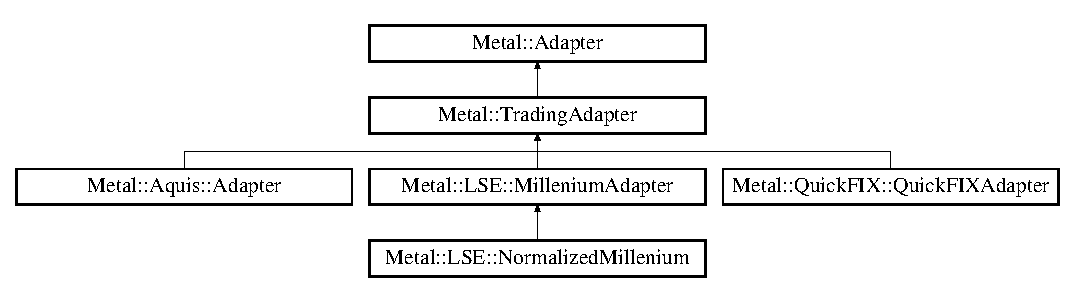
\includegraphics[height=3.000000cm]{classMetal_1_1TradingAdapter}
\end{center}
\end{figure}
\subsection*{Public Member Functions}
\begin{DoxyCompactItemize}
\item 
\hyperlink{classMetal_1_1TradingAdapter_a472ad74753a0bd77a3e78c1f7f8d0398}{Trading\+Adapter} (const std\+::string \&name, const std\+::string \&uuid)
\item 
void \hyperlink{classMetal_1_1TradingAdapter_ae0b309ccc7e9ec5dfe262d071dde4c17}{set\+Remote\+Host} (const std\+::string \&host\+Name, unsigned int port\+Number)
\item 
void \hyperlink{classMetal_1_1TradingAdapter_a1ba0cd89d6475faf9da358140660e886}{start} ()
\item 
void \hyperlink{classMetal_1_1TradingAdapter_aa5e283e9e0a339c738cfba37fed3c7ff}{stop} ()
\item 
void \hyperlink{classMetal_1_1TradingAdapter_ac99cc99c695715fc396756441e68abc0}{send} (\hyperlink{classMetal_1_1Message}{Message} \&msg)
\item 
virtual void \hyperlink{classMetal_1_1TradingAdapter_a2ecc8f1c8fe8a8d29625d142f473f1c3}{send} (const \hyperlink{classMetal_1_1NewOrderSingle}{New\+Order\+Single} \&)=0
\item 
virtual void \hyperlink{classMetal_1_1TradingAdapter_a39562015df3e7202a5e8f932b8bde43e}{send\+Logon} ()=0
\item 
virtual void \hyperlink{classMetal_1_1TradingAdapter_af0015d51815dedb1bc78258b3030d751}{recv} (const Execution\+Report \&er)=0
\item 
virtual void \hyperlink{classMetal_1_1TradingAdapter_a10208ab030e4b3a9db4dc71206a1812e}{on\+Physical\+Connection} ()
\item 
virtual void \hyperlink{classMetal_1_1TradingAdapter_a161ad3db17091807d091d1b236de0105}{benchmark} (const std\+::vector$<$ \hyperlink{classMetal_1_1NewOrderSingle}{New\+Order\+Single} $>$ \&list, std\+::chrono\+::milliseconds \&mapping\+Duration, std\+::chrono\+::milliseconds \&encoding\+Duration)=0
\item 
virtual void \hyperlink{classMetal_1_1TradingAdapter_ae0513f6865414f61a41a8f62bafb0187}{benchmark} (const std\+::vector$<$ \hyperlink{classMetal_1_1OrderCancelRequest}{Order\+Cancel\+Request} $>$ \&list, std\+::chrono\+::milliseconds \&mapping\+Duration, std\+::chrono\+::milliseconds \&encoding\+Duration)=0
\end{DoxyCompactItemize}
\subsection*{Protected Member Functions}
\begin{DoxyCompactItemize}
\item 
void \hyperlink{classMetal_1_1TradingAdapter_a51851f504678002634259b8fd5b22d3e}{close\+Socket} (int delay=0)
\end{DoxyCompactItemize}
\subsection*{Protected Attributes}
\begin{DoxyCompactItemize}
\item 
\hypertarget{classMetal_1_1TradingAdapter_a0948ce848a4bd3f4d48019dde792eb5d}{}std\+::string {\bfseries remote\+Host}\label{classMetal_1_1TradingAdapter_a0948ce848a4bd3f4d48019dde792eb5d}

\item 
\hypertarget{classMetal_1_1TradingAdapter_ac657baf65b2e469f6fa9b641ca50cc21}{}unsigned int {\bfseries remote\+Port}\label{classMetal_1_1TradingAdapter_ac657baf65b2e469f6fa9b641ca50cc21}

\item 
\hypertarget{classMetal_1_1TradingAdapter_a1a742b88c94b305071035985437f49c2}{}N\+L\+::\+Socket $\ast$ {\bfseries socket}\label{classMetal_1_1TradingAdapter_a1a742b88c94b305071035985437f49c2}

\end{DoxyCompactItemize}


\subsection{Constructor \& Destructor Documentation}
\hypertarget{classMetal_1_1TradingAdapter_a472ad74753a0bd77a3e78c1f7f8d0398}{}\index{Metal\+::\+Trading\+Adapter@{Metal\+::\+Trading\+Adapter}!Trading\+Adapter@{Trading\+Adapter}}
\index{Trading\+Adapter@{Trading\+Adapter}!Metal\+::\+Trading\+Adapter@{Metal\+::\+Trading\+Adapter}}
\subsubsection[{Trading\+Adapter}]{\setlength{\rightskip}{0pt plus 5cm}Metal\+::\+Trading\+Adapter\+::\+Trading\+Adapter (
\begin{DoxyParamCaption}
\item[{const std\+::string \&}]{name, }
\item[{const std\+::string \&}]{uuid}
\end{DoxyParamCaption}
)}\label{classMetal_1_1TradingAdapter_a472ad74753a0bd77a3e78c1f7f8d0398}

\begin{DoxyParams}{Parameters}
{\em name} & Whatever should be used to identify this adapter. Subclasses will perform mapping, encoding then write to the active session \\
\hline
\end{DoxyParams}


\subsection{Member Function Documentation}
\hypertarget{classMetal_1_1TradingAdapter_a161ad3db17091807d091d1b236de0105}{}\index{Metal\+::\+Trading\+Adapter@{Metal\+::\+Trading\+Adapter}!benchmark@{benchmark}}
\index{benchmark@{benchmark}!Metal\+::\+Trading\+Adapter@{Metal\+::\+Trading\+Adapter}}
\subsubsection[{benchmark}]{\setlength{\rightskip}{0pt plus 5cm}virtual void Metal\+::\+Trading\+Adapter\+::benchmark (
\begin{DoxyParamCaption}
\item[{const std\+::vector$<$ {\bf New\+Order\+Single} $>$ \&}]{list, }
\item[{std\+::chrono\+::milliseconds \&}]{mapping\+Duration, }
\item[{std\+::chrono\+::milliseconds \&}]{encoding\+Duration}
\end{DoxyParamCaption}
)\hspace{0.3cm}{\ttfamily [pure virtual]}}\label{classMetal_1_1TradingAdapter_a161ad3db17091807d091d1b236de0105}
The purpose is to measure Mapping and Encoding speed for \hyperlink{classMetal_1_1NewOrderSingle}{New\+Order\+Single}~\newline
 Subclasses should make sure to execute both as opposed to just mapping 
\begin{DoxyParams}{Parameters}
{\em list} & A list of \hyperlink{classMetal_1_1NewOrderSingle}{New\+Order\+Single} better if randomly generated \\
\hline
{\em mapping\+Duration} & Time used to map messages \\
\hline
{\em encoding\+Duration} & Time used to encode messages \\
\hline
\end{DoxyParams}


Implemented in \hyperlink{classMetal_1_1QuickFIX_1_1QuickFIXAdapter_ae987b07f906db9fc74d7f7a55eb38efe}{Metal\+::\+Quick\+F\+I\+X\+::\+Quick\+F\+I\+X\+Adapter}.

\hypertarget{classMetal_1_1TradingAdapter_ae0513f6865414f61a41a8f62bafb0187}{}\index{Metal\+::\+Trading\+Adapter@{Metal\+::\+Trading\+Adapter}!benchmark@{benchmark}}
\index{benchmark@{benchmark}!Metal\+::\+Trading\+Adapter@{Metal\+::\+Trading\+Adapter}}
\subsubsection[{benchmark}]{\setlength{\rightskip}{0pt plus 5cm}virtual void Metal\+::\+Trading\+Adapter\+::benchmark (
\begin{DoxyParamCaption}
\item[{const std\+::vector$<$ {\bf Order\+Cancel\+Request} $>$ \&}]{list, }
\item[{std\+::chrono\+::milliseconds \&}]{mapping\+Duration, }
\item[{std\+::chrono\+::milliseconds \&}]{encoding\+Duration}
\end{DoxyParamCaption}
)\hspace{0.3cm}{\ttfamily [pure virtual]}}\label{classMetal_1_1TradingAdapter_ae0513f6865414f61a41a8f62bafb0187}
The purpose is to measure Mapping and Encoding speed for \hyperlink{classMetal_1_1OrderCancelRequest}{Order\+Cancel\+Request}~\newline
 Subclasses should make sure to execute both as opposed to just mapping 
\begin{DoxyParams}{Parameters}
{\em list} & A list of \hyperlink{classMetal_1_1NewOrderSingle}{New\+Order\+Single} better if randomly generated \\
\hline
{\em mapping\+Duration} & Time used to map messages \\
\hline
{\em encoding\+Duration} & Time used to encode messages \\
\hline
\end{DoxyParams}


Implemented in \hyperlink{classMetal_1_1QuickFIX_1_1QuickFIXAdapter_aee108bf917ca43b2a5995c5d2d993e99}{Metal\+::\+Quick\+F\+I\+X\+::\+Quick\+F\+I\+X\+Adapter}.

\hypertarget{classMetal_1_1TradingAdapter_a51851f504678002634259b8fd5b22d3e}{}\index{Metal\+::\+Trading\+Adapter@{Metal\+::\+Trading\+Adapter}!close\+Socket@{close\+Socket}}
\index{close\+Socket@{close\+Socket}!Metal\+::\+Trading\+Adapter@{Metal\+::\+Trading\+Adapter}}
\subsubsection[{close\+Socket}]{\setlength{\rightskip}{0pt plus 5cm}void Metal\+::\+Trading\+Adapter\+::close\+Socket (
\begin{DoxyParamCaption}
\item[{int}]{delay = {\ttfamily 0}}
\end{DoxyParamCaption}
)\hspace{0.3cm}{\ttfamily [protected]}}\label{classMetal_1_1TradingAdapter_a51851f504678002634259b8fd5b22d3e}
This will terminate the physical connection if need be 
\begin{DoxyParams}{Parameters}
{\em delay} & in milliseconds if we should wait before closing \\
\hline
\end{DoxyParams}
\hypertarget{classMetal_1_1TradingAdapter_a10208ab030e4b3a9db4dc71206a1812e}{}\index{Metal\+::\+Trading\+Adapter@{Metal\+::\+Trading\+Adapter}!on\+Physical\+Connection@{on\+Physical\+Connection}}
\index{on\+Physical\+Connection@{on\+Physical\+Connection}!Metal\+::\+Trading\+Adapter@{Metal\+::\+Trading\+Adapter}}
\subsubsection[{on\+Physical\+Connection}]{\setlength{\rightskip}{0pt plus 5cm}void Metal\+::\+Trading\+Adapter\+::on\+Physical\+Connection (
\begin{DoxyParamCaption}
{}
\end{DoxyParamCaption}
)\hspace{0.3cm}{\ttfamily [virtual]}}\label{classMetal_1_1TradingAdapter_a10208ab030e4b3a9db4dc71206a1812e}
This method is invoked once the socket is connected~\newline
 The default behavior is to send a \hyperlink{classMetal_1_1Logon}{Logon} message. Which you may want to override. \hypertarget{classMetal_1_1TradingAdapter_af0015d51815dedb1bc78258b3030d751}{}\index{Metal\+::\+Trading\+Adapter@{Metal\+::\+Trading\+Adapter}!recv@{recv}}
\index{recv@{recv}!Metal\+::\+Trading\+Adapter@{Metal\+::\+Trading\+Adapter}}
\subsubsection[{recv}]{\setlength{\rightskip}{0pt plus 5cm}virtual void Metal\+::\+Trading\+Adapter\+::recv (
\begin{DoxyParamCaption}
\item[{const Execution\+Report \&}]{er}
\end{DoxyParamCaption}
)\hspace{0.3cm}{\ttfamily [pure virtual]}}\label{classMetal_1_1TradingAdapter_af0015d51815dedb1bc78258b3030d751}
This method will invoked upon receiving an execution report~\newline
 Subclasses will perform mapping, encoding then write to the active session~\newline
 
\begin{DoxyParams}{Parameters}
{\em Execution\+Report} & incomming execution report \\
\hline
\end{DoxyParams}


Implemented in \hyperlink{classMetal_1_1LSE_1_1MilleniumAdapter_add4508b367a6383b42fb2fd1744946cd}{Metal\+::\+L\+S\+E\+::\+Millenium\+Adapter}, and \hyperlink{classMetal_1_1QuickFIX_1_1QuickFIXAdapter_a2556160da779a6cde56d52889b9a93db}{Metal\+::\+Quick\+F\+I\+X\+::\+Quick\+F\+I\+X\+Adapter}.

\hypertarget{classMetal_1_1TradingAdapter_ac99cc99c695715fc396756441e68abc0}{}\index{Metal\+::\+Trading\+Adapter@{Metal\+::\+Trading\+Adapter}!send@{send}}
\index{send@{send}!Metal\+::\+Trading\+Adapter@{Metal\+::\+Trading\+Adapter}}
\subsubsection[{send}]{\setlength{\rightskip}{0pt plus 5cm}void Metal\+::\+Trading\+Adapter\+::send (
\begin{DoxyParamCaption}
\item[{{\bf Message} \&}]{msg}
\end{DoxyParamCaption}
)}\label{classMetal_1_1TradingAdapter_ac99cc99c695715fc396756441e68abc0}
This methods sends an message in native format. \hypertarget{classMetal_1_1TradingAdapter_a2ecc8f1c8fe8a8d29625d142f473f1c3}{}\index{Metal\+::\+Trading\+Adapter@{Metal\+::\+Trading\+Adapter}!send@{send}}
\index{send@{send}!Metal\+::\+Trading\+Adapter@{Metal\+::\+Trading\+Adapter}}
\subsubsection[{send}]{\setlength{\rightskip}{0pt plus 5cm}virtual void Metal\+::\+Trading\+Adapter\+::send (
\begin{DoxyParamCaption}
\item[{const {\bf New\+Order\+Single} \&}]{}
\end{DoxyParamCaption}
)\hspace{0.3cm}{\ttfamily [pure virtual]}}\label{classMetal_1_1TradingAdapter_a2ecc8f1c8fe8a8d29625d142f473f1c3}
This method will be called by users to send new orders~\newline
 Subclasses will perform mapping, encoding then write to the active session~\newline
 
\begin{DoxyParams}{Parameters}
{\em \hyperlink{classMetal_1_1NewOrderSingle}{New\+Order\+Single}} & Inbound order in unified format \\
\hline
\end{DoxyParams}
\begin{DoxySeeAlso}{See also}
\hyperlink{classMetal_1_1NewOrderSingle}{New\+Order\+Single} 
\end{DoxySeeAlso}


Implemented in \hyperlink{classMetal_1_1LSE_1_1MilleniumAdapter_ab3da43142636043e0ade20b0881c9976}{Metal\+::\+L\+S\+E\+::\+Millenium\+Adapter}, and \hyperlink{classMetal_1_1QuickFIX_1_1QuickFIXAdapter_afda717ce98408850ccd9b7a2c953aedd}{Metal\+::\+Quick\+F\+I\+X\+::\+Quick\+F\+I\+X\+Adapter}.

\hypertarget{classMetal_1_1TradingAdapter_a39562015df3e7202a5e8f932b8bde43e}{}\index{Metal\+::\+Trading\+Adapter@{Metal\+::\+Trading\+Adapter}!send\+Logon@{send\+Logon}}
\index{send\+Logon@{send\+Logon}!Metal\+::\+Trading\+Adapter@{Metal\+::\+Trading\+Adapter}}
\subsubsection[{send\+Logon}]{\setlength{\rightskip}{0pt plus 5cm}virtual void Metal\+::\+Trading\+Adapter\+::send\+Logon (
\begin{DoxyParamCaption}
{}
\end{DoxyParamCaption}
)\hspace{0.3cm}{\ttfamily [pure virtual]}}\label{classMetal_1_1TradingAdapter_a39562015df3e7202a5e8f932b8bde43e}
This pure virtual method should be implemented in each adapter. 

Implemented in \hyperlink{classMetal_1_1LSE_1_1MilleniumAdapter_ab4bba2e8403ae7ed5b335985b4295b9f}{Metal\+::\+L\+S\+E\+::\+Millenium\+Adapter}, and \hyperlink{classMetal_1_1QuickFIX_1_1QuickFIXAdapter_a3f9dba36bbaa3d8db8af62ac07a9fff5}{Metal\+::\+Quick\+F\+I\+X\+::\+Quick\+F\+I\+X\+Adapter}.

\hypertarget{classMetal_1_1TradingAdapter_ae0b309ccc7e9ec5dfe262d071dde4c17}{}\index{Metal\+::\+Trading\+Adapter@{Metal\+::\+Trading\+Adapter}!set\+Remote\+Host@{set\+Remote\+Host}}
\index{set\+Remote\+Host@{set\+Remote\+Host}!Metal\+::\+Trading\+Adapter@{Metal\+::\+Trading\+Adapter}}
\subsubsection[{set\+Remote\+Host}]{\setlength{\rightskip}{0pt plus 5cm}void Metal\+::\+Trading\+Adapter\+::set\+Remote\+Host (
\begin{DoxyParamCaption}
\item[{const std\+::string \&}]{host\+Name, }
\item[{unsigned int}]{port\+Number}
\end{DoxyParamCaption}
)}\label{classMetal_1_1TradingAdapter_ae0b309ccc7e9ec5dfe262d071dde4c17}
This method should be invoked before starting the adapter to set remote host properties 
\begin{DoxyParams}{Parameters}
{\em host\+Name} & name of the remote host \\
\hline
{\em port\+Number} & remote port number \\
\hline
\end{DoxyParams}
\hypertarget{classMetal_1_1TradingAdapter_a1ba0cd89d6475faf9da358140660e886}{}\index{Metal\+::\+Trading\+Adapter@{Metal\+::\+Trading\+Adapter}!start@{start}}
\index{start@{start}!Metal\+::\+Trading\+Adapter@{Metal\+::\+Trading\+Adapter}}
\subsubsection[{start}]{\setlength{\rightskip}{0pt plus 5cm}void Metal\+::\+Trading\+Adapter\+::start (
\begin{DoxyParamCaption}
{}
\end{DoxyParamCaption}
)\hspace{0.3cm}{\ttfamily [virtual]}}\label{classMetal_1_1TradingAdapter_a1ba0cd89d6475faf9da358140660e886}
This function should be invoked to initiate physical connection~\newline
 It will create a new Thread for incomming messages 

Implements \hyperlink{classMetal_1_1Adapter}{Metal\+::\+Adapter}.

\hypertarget{classMetal_1_1TradingAdapter_aa5e283e9e0a339c738cfba37fed3c7ff}{}\index{Metal\+::\+Trading\+Adapter@{Metal\+::\+Trading\+Adapter}!stop@{stop}}
\index{stop@{stop}!Metal\+::\+Trading\+Adapter@{Metal\+::\+Trading\+Adapter}}
\subsubsection[{stop}]{\setlength{\rightskip}{0pt plus 5cm}void Metal\+::\+Trading\+Adapter\+::stop (
\begin{DoxyParamCaption}
{}
\end{DoxyParamCaption}
)\hspace{0.3cm}{\ttfamily [virtual]}}\label{classMetal_1_1TradingAdapter_aa5e283e9e0a339c738cfba37fed3c7ff}
This method will close logical and physical connection~\newline
 All created threads will be terminated 

Implements \hyperlink{classMetal_1_1Adapter}{Metal\+::\+Adapter}.



The documentation for this class was generated from the following files\+:\begin{DoxyCompactItemize}
\item 
/home/jc/metal/src/metal/Trading\+Adapter.\+h\item 
/home/jc/metal/src/metal/Trading\+Adapter.\+cpp\end{DoxyCompactItemize}

\hypertarget{classMetal_1_1Translator}{}\section{Metal\+:\+:Translator Class Reference}
\label{classMetal_1_1Translator}\index{Metal\+::\+Translator@{Metal\+::\+Translator}}


{\ttfamily \#include $<$Translator.\+h$>$}

\subsection*{Public Member Functions}
\begin{DoxyCompactItemize}
\item 
\hyperlink{classMetal_1_1Translator_a030bdd567db5d505e04e1fe64fda174d}{Translator} ()
\item 
virtual \hyperlink{classMetal_1_1Translator_ac9e56b0e458e14558a3512f889e24dc1}{$\sim$\+Translator} ()
\end{DoxyCompactItemize}
\subsection*{Static Public Member Functions}
\begin{DoxyCompactItemize}
\item 
static const std\+::string \hyperlink{classMetal_1_1Translator_a3a9953b65baf38dbc4c2ea835a005cf5}{field} (const F\+I\+X\+::\+Ord\+Status \&)
\item 
static const std\+::string \hyperlink{classMetal_1_1Translator_a726f01b6ba7f36a0c77ab2fb098acf37}{field} (const F\+I\+X\+::\+Exec\+Type \&)
\item 
static const std\+::string \hyperlink{classMetal_1_1Translator_a8297f6329e8de18e50547746ea84ee59}{field} (const F\+I\+X\+::\+Side \&)
\end{DoxyCompactItemize}


\subsection{Detailed Description}
This class is meant to translate F\+I\+X field values into plain English 

\subsection{Constructor \& Destructor Documentation}
\hypertarget{classMetal_1_1Translator_a030bdd567db5d505e04e1fe64fda174d}{}\index{Metal\+::\+Translator@{Metal\+::\+Translator}!Translator@{Translator}}
\index{Translator@{Translator}!Metal\+::\+Translator@{Metal\+::\+Translator}}
\subsubsection[{Translator}]{\setlength{\rightskip}{0pt plus 5cm}Metal\+::\+Translator\+::\+Translator (
\begin{DoxyParamCaption}
{}
\end{DoxyParamCaption}
)}\label{classMetal_1_1Translator_a030bdd567db5d505e04e1fe64fda174d}
\hypertarget{classMetal_1_1Translator_ac9e56b0e458e14558a3512f889e24dc1}{}\index{Metal\+::\+Translator@{Metal\+::\+Translator}!````~Translator@{$\sim$\+Translator}}
\index{````~Translator@{$\sim$\+Translator}!Metal\+::\+Translator@{Metal\+::\+Translator}}
\subsubsection[{$\sim$\+Translator}]{\setlength{\rightskip}{0pt plus 5cm}Metal\+::\+Translator\+::$\sim$\+Translator (
\begin{DoxyParamCaption}
{}
\end{DoxyParamCaption}
)\hspace{0.3cm}{\ttfamily [virtual]}}\label{classMetal_1_1Translator_ac9e56b0e458e14558a3512f889e24dc1}


\subsection{Member Function Documentation}
\hypertarget{classMetal_1_1Translator_a3a9953b65baf38dbc4c2ea835a005cf5}{}\index{Metal\+::\+Translator@{Metal\+::\+Translator}!field@{field}}
\index{field@{field}!Metal\+::\+Translator@{Metal\+::\+Translator}}
\subsubsection[{field}]{\setlength{\rightskip}{0pt plus 5cm}const std\+::string Metal\+::\+Translator\+::field (
\begin{DoxyParamCaption}
\item[{const F\+I\+X\+::\+Ord\+Status \&}]{ord\+Status}
\end{DoxyParamCaption}
)\hspace{0.3cm}{\ttfamily [static]}}\label{classMetal_1_1Translator_a3a9953b65baf38dbc4c2ea835a005cf5}
\hypertarget{classMetal_1_1Translator_a726f01b6ba7f36a0c77ab2fb098acf37}{}\index{Metal\+::\+Translator@{Metal\+::\+Translator}!field@{field}}
\index{field@{field}!Metal\+::\+Translator@{Metal\+::\+Translator}}
\subsubsection[{field}]{\setlength{\rightskip}{0pt plus 5cm}const std\+::string Metal\+::\+Translator\+::field (
\begin{DoxyParamCaption}
\item[{const F\+I\+X\+::\+Exec\+Type \&}]{exec\+Type}
\end{DoxyParamCaption}
)\hspace{0.3cm}{\ttfamily [static]}}\label{classMetal_1_1Translator_a726f01b6ba7f36a0c77ab2fb098acf37}
\hypertarget{classMetal_1_1Translator_a8297f6329e8de18e50547746ea84ee59}{}\index{Metal\+::\+Translator@{Metal\+::\+Translator}!field@{field}}
\index{field@{field}!Metal\+::\+Translator@{Metal\+::\+Translator}}
\subsubsection[{field}]{\setlength{\rightskip}{0pt plus 5cm}const std\+::string Metal\+::\+Translator\+::field (
\begin{DoxyParamCaption}
\item[{const F\+I\+X\+::\+Side \&}]{side}
\end{DoxyParamCaption}
)\hspace{0.3cm}{\ttfamily [static]}}\label{classMetal_1_1Translator_a8297f6329e8de18e50547746ea84ee59}


The documentation for this class was generated from the following files\+:\begin{DoxyCompactItemize}
\item 
/home/jc/metal/github/include/metal/\hyperlink{Translator_8h}{Translator.\+h}\item 
/home/jc/metal/github/src/metal/\hyperlink{Translator_8cpp}{Translator.\+cpp}\end{DoxyCompactItemize}

\chapter{File Documentation}
\hypertarget{core_8h}{}\section{/home/jc/metal/src/net\+Link/include/netlink/core.h File Reference}
\label{core_8h}\index{/home/jc/metal/src/net\+Link/include/netlink/core.\+h@{/home/jc/metal/src/net\+Link/include/netlink/core.\+h}}
{\ttfamily \#include \char`\"{}netlink/config.\+h\char`\"{}}\\*
{\ttfamily \#include $<$arpa/inet.\+h$>$}\\*
{\ttfamily \#include $<$sys/fcntl.\+h$>$}\\*
{\ttfamily \#include $<$sys/types.\+h$>$}\\*
{\ttfamily \#include $<$sys/socket.\+h$>$}\\*
{\ttfamily \#include $<$sys/unistd.\+h$>$}\\*
{\ttfamily \#include $<$sys/time.\+h$>$}\\*
{\ttfamily \#include $<$netdb.\+h$>$}\\*
{\ttfamily \#include $<$sys/ioctl.\+h$>$}\\*
{\ttfamily \#include $<$errno.\+h$>$}\\*
{\ttfamily \#include $<$string$>$}\\*
{\ttfamily \#include \char`\"{}netlink/exception.\+h\char`\"{}}\\*
{\ttfamily \#include \char`\"{}netlink/release\+\_\+manager.\+h\char`\"{}}\\*
{\ttfamily \#include \char`\"{}netlink/util.\+h\char`\"{}}\\*
\subsection*{Macros}
\begin{DoxyCompactItemize}
\item 
\hypertarget{core_8h_abc19f1dd7f7e0c32a2dfc5157066db0a}{}\#define {\bfseries N\+L\+\_\+\+N\+A\+M\+E\+S\+P\+A\+C\+E\+\_\+\+N\+A\+M\+E}~N\+L\label{core_8h_abc19f1dd7f7e0c32a2dfc5157066db0a}

\item 
\hypertarget{core_8h_a534bbab9b8761b1ec5420d4b8a9bbd11}{}\#define {\bfseries N\+L\+\_\+\+N\+A\+M\+E\+S\+P\+A\+C\+E}~namespace N\+L\+\_\+\+N\+A\+M\+E\+S\+P\+A\+C\+E\+\_\+\+N\+A\+M\+E \{\label{core_8h_a534bbab9b8761b1ec5420d4b8a9bbd11}

\item 
\hypertarget{core_8h_ae1a7a99e2ba26685d2c01ce44709b9d7}{}\#define {\bfseries N\+L\+\_\+\+N\+A\+M\+E\+S\+P\+A\+C\+E\+\_\+\+E\+N\+D}~\};\label{core_8h_ae1a7a99e2ba26685d2c01ce44709b9d7}

\item 
\hypertarget{core_8h_a72e3e989b9baebd5f7c04922fae6e589}{}\#define {\bfseries N\+L\+\_\+\+N\+A\+M\+E\+S\+P\+A\+C\+E\+\_\+\+U\+S\+E}~using namespace N\+L\+\_\+\+N\+A\+M\+E\+S\+P\+A\+C\+E\+\_\+\+N\+A\+M\+E;\label{core_8h_a72e3e989b9baebd5f7c04922fae6e589}

\item 
\hypertarget{core_8h_ae273c7db78098028c7a6b6b230ac0503}{}\#define {\bfseries O\+S\+\_\+\+L\+I\+N\+U\+X}\label{core_8h_ae273c7db78098028c7a6b6b230ac0503}

\end{DoxyCompactItemize}
\subsection*{Enumerations}
\begin{DoxyCompactItemize}
\item 
enum \hyperlink{core_8h_aac39b55be6469395f55ff0292ad8184c}{Protocol} \{ \hyperlink{core_8h_aac39b55be6469395f55ff0292ad8184caa040cd7feeb588104634cdadf35abf1c}{T\+C\+P}, 
\hyperlink{core_8h_aac39b55be6469395f55ff0292ad8184cadb542475cf9d0636e4225e216cee9ae6}{U\+D\+P}
 \}
\item 
enum \hyperlink{core_8h_a3afbe2755e4a6912bfce39e7069c2d3d}{I\+P\+Ver} \{ \hyperlink{core_8h_a3afbe2755e4a6912bfce39e7069c2d3da7cecc0cd33e7aadefd2826553c9e634e}{I\+P4}, 
\hyperlink{core_8h_a3afbe2755e4a6912bfce39e7069c2d3dabf4c53a0c24e17362bbe8ecb0347e4e6}{I\+P6}, 
\hyperlink{core_8h_a3afbe2755e4a6912bfce39e7069c2d3daa00374190265e7b6447db44977a7dff1}{A\+N\+Y}
 \}
\item 
enum \hyperlink{core_8h_aa78c7398fa81f7f62aa233159d4d8d97}{Socket\+Type} \{ \hyperlink{core_8h_aa78c7398fa81f7f62aa233159d4d8d97a48e4cb37544c8e69715d45e5a83b2109}{C\+L\+I\+E\+N\+T}, 
\hyperlink{core_8h_aa78c7398fa81f7f62aa233159d4d8d97a67c96b24b23bcb408bae7626730a04b7}{S\+E\+R\+V\+E\+R}
 \}
\end{DoxyCompactItemize}
\subsection*{Functions}
\begin{DoxyCompactItemize}
\item 
void \hyperlink{core_8h_a9b878fee41d5996021dea123e7d071b4}{init} ()
\end{DoxyCompactItemize}


\subsection{Detailed Description}
Net\+Link core types and init 

\subsection{Enumeration Type Documentation}
\hypertarget{core_8h_a3afbe2755e4a6912bfce39e7069c2d3d}{}\index{core.\+h@{core.\+h}!I\+P\+Ver@{I\+P\+Ver}}
\index{I\+P\+Ver@{I\+P\+Ver}!core.\+h@{core.\+h}}
\subsubsection[{I\+P\+Ver}]{\setlength{\rightskip}{0pt plus 5cm}enum {\bf I\+P\+Ver}}\label{core_8h_a3afbe2755e4a6912bfce39e7069c2d3d}
Defines the version of I\+P. \begin{Desc}
\item[Enumerator]\par
\begin{description}
\index{I\+P4@{I\+P4}!core.\+h@{core.\+h}}\index{core.\+h@{core.\+h}!I\+P4@{I\+P4}}\item[{\em 
\hypertarget{core_8h_a3afbe2755e4a6912bfce39e7069c2d3da7cecc0cd33e7aadefd2826553c9e634e}{}I\+P4\label{core_8h_a3afbe2755e4a6912bfce39e7069c2d3da7cecc0cd33e7aadefd2826553c9e634e}
}]I\+P version 4 \index{I\+P6@{I\+P6}!core.\+h@{core.\+h}}\index{core.\+h@{core.\+h}!I\+P6@{I\+P6}}\item[{\em 
\hypertarget{core_8h_a3afbe2755e4a6912bfce39e7069c2d3dabf4c53a0c24e17362bbe8ecb0347e4e6}{}I\+P6\label{core_8h_a3afbe2755e4a6912bfce39e7069c2d3dabf4c53a0c24e17362bbe8ecb0347e4e6}
}]I\+P version 6 \index{A\+N\+Y@{A\+N\+Y}!core.\+h@{core.\+h}}\index{core.\+h@{core.\+h}!A\+N\+Y@{A\+N\+Y}}\item[{\em 
\hypertarget{core_8h_a3afbe2755e4a6912bfce39e7069c2d3daa00374190265e7b6447db44977a7dff1}{}A\+N\+Y\label{core_8h_a3afbe2755e4a6912bfce39e7069c2d3daa00374190265e7b6447db44977a7dff1}
}]Any I\+P version \end{description}
\end{Desc}
\hypertarget{core_8h_aac39b55be6469395f55ff0292ad8184c}{}\index{core.\+h@{core.\+h}!Protocol@{Protocol}}
\index{Protocol@{Protocol}!core.\+h@{core.\+h}}
\subsubsection[{Protocol}]{\setlength{\rightskip}{0pt plus 5cm}enum {\bf Protocol}}\label{core_8h_aac39b55be6469395f55ff0292ad8184c}
Defines protocol type. \begin{Desc}
\item[Enumerator]\par
\begin{description}
\index{T\+C\+P@{T\+C\+P}!core.\+h@{core.\+h}}\index{core.\+h@{core.\+h}!T\+C\+P@{T\+C\+P}}\item[{\em 
\hypertarget{core_8h_aac39b55be6469395f55ff0292ad8184caa040cd7feeb588104634cdadf35abf1c}{}T\+C\+P\label{core_8h_aac39b55be6469395f55ff0292ad8184caa040cd7feeb588104634cdadf35abf1c}
}]T\+C\+P Protocol \index{U\+D\+P@{U\+D\+P}!core.\+h@{core.\+h}}\index{core.\+h@{core.\+h}!U\+D\+P@{U\+D\+P}}\item[{\em 
\hypertarget{core_8h_aac39b55be6469395f55ff0292ad8184cadb542475cf9d0636e4225e216cee9ae6}{}U\+D\+P\label{core_8h_aac39b55be6469395f55ff0292ad8184cadb542475cf9d0636e4225e216cee9ae6}
}]U\+D\+P Protocol \end{description}
\end{Desc}
\hypertarget{core_8h_aa78c7398fa81f7f62aa233159d4d8d97}{}\index{core.\+h@{core.\+h}!Socket\+Type@{Socket\+Type}}
\index{Socket\+Type@{Socket\+Type}!core.\+h@{core.\+h}}
\subsubsection[{Socket\+Type}]{\setlength{\rightskip}{0pt plus 5cm}enum {\bf Socket\+Type}}\label{core_8h_aa78c7398fa81f7f62aa233159d4d8d97}
Defines the nature of the socket. \begin{Desc}
\item[Enumerator]\par
\begin{description}
\index{C\+L\+I\+E\+N\+T@{C\+L\+I\+E\+N\+T}!core.\+h@{core.\+h}}\index{core.\+h@{core.\+h}!C\+L\+I\+E\+N\+T@{C\+L\+I\+E\+N\+T}}\item[{\em 
\hypertarget{core_8h_aa78c7398fa81f7f62aa233159d4d8d97a48e4cb37544c8e69715d45e5a83b2109}{}C\+L\+I\+E\+N\+T\label{core_8h_aa78c7398fa81f7f62aa233159d4d8d97a48e4cb37544c8e69715d45e5a83b2109}
}]T\+C\+P or U\+D\+P socket connected or directed to a target host \index{S\+E\+R\+V\+E\+R@{S\+E\+R\+V\+E\+R}!core.\+h@{core.\+h}}\index{core.\+h@{core.\+h}!S\+E\+R\+V\+E\+R@{S\+E\+R\+V\+E\+R}}\item[{\em 
\hypertarget{core_8h_aa78c7398fa81f7f62aa233159d4d8d97a67c96b24b23bcb408bae7626730a04b7}{}S\+E\+R\+V\+E\+R\label{core_8h_aa78c7398fa81f7f62aa233159d4d8d97a67c96b24b23bcb408bae7626730a04b7}
}]T\+C\+P socket which listens for connections or U\+D\+P socket without target host \end{description}
\end{Desc}


\subsection{Function Documentation}
\hypertarget{core_8h_a9b878fee41d5996021dea123e7d071b4}{}\index{core.\+h@{core.\+h}!init@{init}}
\index{init@{init}!core.\+h@{core.\+h}}
\subsubsection[{init}]{\setlength{\rightskip}{0pt plus 5cm}N\+L\+\_\+\+N\+A\+M\+E\+S\+P\+A\+C\+Evoid init (
\begin{DoxyParamCaption}
{}
\end{DoxyParamCaption}
)}\label{core_8h_a9b878fee41d5996021dea123e7d071b4}
Library initialization function

\begin{DoxyWarning}{Warning}
Must be called before using the library 
\end{DoxyWarning}

\chapter{Example Documentation}
\hypertarget{chatClient_8cc-example}{}\section{chat\+Client.\+cc}
Example of \hyperlink{classSocketGroup}{Socket\+Group}


\begin{DoxyCodeInclude}
\end{DoxyCodeInclude}
 
\hypertarget{chatServer_8cc-example}{}\section{chat\+Server.\+cc}
Example of \hyperlink{classSocketGroup}{Socket\+Group}


\begin{DoxyCodeInclude}
\end{DoxyCodeInclude}
 
\hypertarget{clientEcho_8cc-example}{}\section{client\+Echo.\+cc}
Example of T\+C\+P C\+L\+I\+E\+N\+T \hyperlink{classSocket}{Socket}


\begin{DoxyCodeInclude}
\end{DoxyCodeInclude}
 
\hypertarget{serverEcho_8cc-example}{}\section{server\+Echo.\+cc}
Example of T\+C\+P S\+E\+R\+V\+E\+R \hyperlink{classSocket}{Socket}


\begin{DoxyCodeInclude}
\end{DoxyCodeInclude}
 
\hypertarget{udpDirectChat_8cc-example}{}\section{udp\+Direct\+Chat.\+cc}
Example of U\+D\+P non-\/blocking \hyperlink{classSocket}{Socket}


\begin{DoxyCodeInclude}
\end{DoxyCodeInclude}
 
\hypertarget{webGet_8cc-example}{}\section{web\+Get.\+cc}
Example of \hyperlink{classSmartBuffer}{Smart\+Buffer} and \hyperlink{classSocketGroup}{Socket\+Group}. Retrieves a web page and prints it.


\begin{DoxyCodeInclude}
\end{DoxyCodeInclude}
 
%--- End generated contents ---

% Index
\backmatter
\newpage
\phantomsection
\clearemptydoublepage
\addcontentsline{toc}{chapter}{Index}
\printindex

\end{document}
